\documentclass[MSc]{abdnthesis}

%% For citations, I would recommend natbib for its
%% flexibility, particularly when named citation styles are used, but
%% it also has useful features for plain and those of that ilk.
%% The natbib package gives you the following definitons
%% that extend the simple \cite:
%   \citet{key} ==>>                Jones et al. (1990)
%   \citet*{key} ==>>               Jones, Baker, and Smith (1990)
%   \citep{key} ==>>                (Jones et al., 1990)
%   \citep*{key} ==>>               (Jones, Baker, and Smith, 1990)
%   \citep[chap. 2]{key} ==>>       (Jones et al., 1990, chap. 2)
%   \citep[e.g.][]{key} ==>>        (e.g. Jones et al., 1990)
%   \citep[e.g.][p. 32]{key} ==>>   (e.g. Jones et al., p. 32)
%   \citeauthor{key} ==>>           Jones et al.
%   \citeauthor*{key} ==>>          Jones, Baker, and Smith
%   \citeyear{key} ==>>             1990

\usepackage[round,colon,authoryear]{natbib}
\setlength{\bibsep}{0pt}
\bibliographystyle{apalike}

\usepackage{array}
\usepackage{xcolor}
\usepackage[T1]{fontenc}
\usepackage{amsmath,amsfonts}
\usepackage{subcaption}
\usepackage{rotating} % for sidewaysfigure to rotate wide figures
\usepackage[export]{adjustbox} % enable relative trim/clip for includegraphics
\usepackage{seqsplit}
\usepackage{pdflscape}
\usepackage{geometry}
\usepackage{hyperref}
\usepackage{tikz}
\usepackage{listings}
\lstset{
  basicstyle=\ttfamily\small,
  breaklines=true,
  frame=single,
  columns=fullflexible
}
\usetikzlibrary{shadows,arrows.meta}

% \title{Research on Application of Pure Visual SLAM Based on Stereo Camera in Edge Computing Lightweight Embedded System}

\title{Pure Vision SLAM Engineering in Robotic Edge Computing Systems}

\author{Jian Chen}

\school{Department of Computing Science}


\date{2025}

\def\sfthing#1#2{\def#1{\mbox{{\small\normalfont\sffamily #2}}}}

\sfthing{\PP}{P}
\sfthing{\FF}{F}



\begin{document}

%%%% Create the title page and standard declaration.

\maketitle
\makedeclaration

%%%% Then the abstract and acknowledgements

\begin{abstract}
  % An expansion of the title and contraction of the thesis.
  % 中文版：
  % 本论文介绍了一种基于双目相机的机器人纯视觉SLAM（Simultaneous Localization and Mapping）系统的工程实现，该系统专为边缘计算轻量级嵌入式系统设计。研究重点在于视觉SLAM技术在机器人领域的实际应用，强调了双目视觉、边缘计算和轻量级。
  % 软件架构方面，整个软件架构构建于Ubuntu 22.04 LTS 之上，使用Humble版本的ROS2作为通信中间件，在ROS2上构建了Turtlebot3_bringup包、zed-ros2包、rtabmap-ros2包、uoa_robot_drone包、rviz2包和navigation2等包。系统的主要功能包括机器人控制模块、双目视觉图像采集模块、图像格式转换与压缩传输模块、视觉SLAM算法模块、定位监控与发布模块、无人机自动投递模块、导航模块和可视化模块。该系统旨在实时处理双目图像，创建环境地图，同时跟踪机器人在该地图中的位置。实现过程中采用了边缘计算原则，以确保低延迟和高效率，使其适用于资源受限的嵌入式系统部署。
  % 硬件方面，机器人地盘用的是Turtlebot3 Waffle Pi (SBC:Raspberry Pi Model 4B, OpenCR:STM32F746ZGT6 / 32-bit ARM Cortex®-M7 with FPU (216MHz, 462DMIPS),电池：MVMOD 3S, 2200 mAh 11.1 V 35C Lipo Battery), 嵌入式边缘计算单元用的是Jetson Orin Nano (最大功耗15W, 电池：INIU 65W 20000mAh Power Bank)，相机用的是ZED 2双目相机(分辨率使用VGA，贞率使用15Hz)，远程监控用的是联想Yoga 14S笔记本电脑(处理器: Intel Core i5-1165G7, 内存: 16GB LPDDR4x, 存储: 512GB SSD)，无人机用的是DJI Tello EDU版，设备间通信用的是手机热点(建图、定位、导航阶段用的是5GHz WiFi, 投递阶段用的是2.4GHz WiFi (因为Tello只支持2.4GHz))。
  % 效果：可以实现实时的地图构建和定位，无人机自动投递等任务。该系统展示了边缘计算在机器人视觉SLAM中的应用潜力。
  % The software architecture involved in this engineering project consists of several key componets, including a robotic control module, a stereo vision image capture module, an image format converting and compression and transmission module, a visual SLAM algorithm module, a localization monitoring and publisher module, a auto delivery with drone module, a navigation module, and a visual lization module. The system is designed to operate in real-time, processing stereo images to create a map of the environment while simultaneously tracking the robot's position within that map. The implementation leverages edge computing principles to ensure low latency and high efficiency, making it suitable for deployment in resource-constrained embedded systems.
  % English version:
  This thesis presents the engineering implementation of a robotic pure vision SLAM (Simultaneous Localization and Mapping) system based on a stereo camera, designed for edge computing embedded systems. The work focuses on the practical application of visual SLAM techniques in robotics, emphasizing the integration of stereo vision, edge computing, and lightweight embedded systems to achieve efficient and effective mapping, localization, multi-agent (robot and drone) collaboration, and navigation in real-time environments.
  
  In terms of software architecture, the system is built on Ubuntu 22.04 LTS, utilizing ROS2 Humble as the middleware. Key packages include Turtlebot3\_bringup, zed-ros2, rtabmap-ros2, uoa\_robot\_drone, rviz2, and navigation2. The main functionalities encompass a robotic control module, stereo vision image capture module, image format conversion and compression transmission module, visual SLAM algorithm module, localization monitoring and publishing module, automated drone delivery module, navigation module, and visualization module. The system aims to process stereo images in real-time to create an environmental map while tracking the robot's position within that map. The implementation adheres to edge computing principles to ensure low latency and high efficiency, making it suitable for deployment in resource-constrained embedded systems.
  
  The hardware setup includes a Turtlebot3 Waffle Pi robot base (SBC: Raspberry Pi Model 4B, OpenCR: STM32F746ZGT6 / 32-bit ARM Cortex, Battery: MVMOD 3S, 2200 mAh 11.1 V 35C Lipo Battery), an embedded edge computing unit using Jetson Orin Nano (max power 15W, Battery: INIU 65W 20000mAh Power Bank), a ZED 2 stereo camera (resolution set to VGA, frame rate set to 15Hz), a Lenovo Yoga 14S laptop for remote monitoring (Processor: Intel Core i5-1165G7, Memory: 16GB LPDDR4x, Storage: 512GB SSD), and a DJI Tello EDU drone for delivery tasks. The communication between devices is facilitated through a mobile hotspot, utilizing 5GHz WiFi during mapping, localization, and navigation phases, and switching to 2.4GHz WiFi for the delivery phase due to the Tello's compatibility.
  
  The system successfully demonstrates real-time mapping and localization capabilities, along with automated drone delivery tasks. This project showcases the potential of edge computing in robotic visual SLAM applications and demonstrates the process of engineering mathematics, computer science, AI and other related knowledge into products.

\end{abstract}

\begin{acknowledgements}
  % 中文版：
  % 我首先感谢我的家人和我北京大学的恩师孙加肃教授，是你们的支持让我最终决定在工作多年后重返校园进行全日制、系统化地学习AI领域的知识。感谢阿伯丁大学的易德伟教授，不仅教授了我机器学习、AI应用两门课程，而且在我做本毕业项目的过程中启发了我通过工程化思路将所学到的数学、计算机、AI等理论知识转化为产品从而提升现实生活中的生产力的诸多灵感,让我在该项目过程中极大提升了将机器人工作原理、纯双目视觉SLAM、神经网络、边缘计算、嵌入式系统、导航算法等理论知识通过工程化方式转化为具体产品的能力。
  % 我还要按授课顺序依次感谢教授我AI课程的各位教授、讲师，是他们让我系统地学习了AI领域的相关专业知识，他们是教授我Symbolic AI课程的Felipe Meneguzzi教授、Yaji Sripada博士，与易德伟教授一起教授我Machine Learning和Applied Artificial Intelligence两门课程的钟明军博士，教授我Evaluation of AI Systems 课程的赵伟博士，共同教授我Software Agents And Multi-Agent Systems 和 Knowledge Representation And Reasoning两门课程的Rafael Cardoso博士和Leonardo Amado博士，与Yaji Sripada博士一起教授我Natural Language Generation课程的Ehud Reiter教授，以及教授我Data Mining with Deep Learning课程的Arabella Sinclair 博士。
  % 今后我会将更多的AI领域的知识通过工程化的方式应用到产品中去，让这些知识在推动人类生产力发展方面发挥更大作用，这或许是对大家最好的感谢方式！
  
  % English version:
  I would like to express my sincere gratitude to all those who have supported me throughout this research journey.
  
  First and foremost, I am deeply grateful to my family and my mentor Professor Jiasu Sun from Peking University, whose unwavering support enabled me to make the decision to return to university campus for full-time, systematic study in the field of Artificial Intelligence after years of professional work in industry.
  
  I extend my heartfelt thanks to Professor Dewei Yi at the University of Aberdeen, who not only taught me \textit{Machine Learning} and \textit{Applied Artificial Intelligence} courses, but also inspired me during this dissertation project to transform theoretical knowledge in mathematics, computer science, and AI into practical engineering solutions that enhance real-world productivity. Through this project, I have significantly improved my ability to convert theoretical concepts in robotics, stereo visual SLAM, neural networks, edge computing, embedded systems, and navigation algorithms into concrete products through engineering approaches.
  
  I would also like to acknowledge, in chronological order of instruction, all the professors and lecturers who taught me AI courses and provided me with systematic knowledge in the field of Artificial Intelligence: Professor Felipe Meneguzzi and Dr. Yaji Sripada for \textit{Symbolic AI}; Dr. Mingjun Zhong, who together with Professor Dewei Yi taught \textit{Machine Learning} and \textit{Applied Artificial Intelligence}; Dr. Wei Zhao for \textit{Evaluation of AI Systems}; Dr. Rafael Cardoso and Dr. Leonardo Amado for \textit{Software Agents and Multi-Agent Systems}, and \textit{Knowledge Representation and Reasoning}; Professor Ehud Reiter, who together with Dr. Yaji Sripada taught \textit{Natural Language Generation}; and Dr. Arabella Sinclair for \textit{Data Mining with Deep Learning}.
  
  Looking forward, I am committed to applying AI knowledge through engineering approaches to develop practical products that contribute to human productivity advancement, which I believe is the best way to honor the education and guidance I have received from all these remarkable educators.
\end{acknowledgements}

\tableofcontents


\chapter{Introduction\label{chap:introduction}}
% 中文版思路：
% 在人工智能和机器人领域，工程实施是数学模型、算法创新和实际生产力提升之间的关键桥梁。当复杂的数学公式和人工智能理论框架通过工程方法有效地转化为实际产品时，其推动人类生产力发展的潜力将得到更充分的体现。多年来，机器人领域出现了各种版本的定位与地图构建技术，比如：Gmapping、Cartographer、ORB-SLAM、FAST-LIO、VINS-Mono、VINS-Fusion等。 
% 本论文阐述了一个将基于双目相机的纯视觉SLAM技术工程化为室内递送系统产品的过程。本阶段，该系统产品的功能包括3个方面：
% 1. 室内机器人进行同时定位与建图；
% 2. 建图完成后，机器人在室内行走时，可以在地图上实时反映出机器人的位置；
% 3. 设定一个目标位置，当机器人到达目标位置时，无人机可以自动起飞运送货物到目的地；
% 未来工作：
% 1.设定一个目标位置，机器人可以自动导航至目的地；
% 2.将该送货系统的工作场景，扩展至室外。
% 该工程使用的硬件设备主要有：Turtlebot3 Waffle Pi, ZED 2 双目相机，边缘计算单元Jetson Orin Nano (Max power 15W), Battery: INIU 65W 20000mAh Power Bank, 大疆Tello EDU版无人机；监控系统使用一台一般的内存16GB的笔记本电脑或PC机即可。软件模块主要有Ubuntu 22.04 LTS Server (用于Raspberry Pi SBC的操作系统), 本文接下来将从系统选型、系统设计、系统实现、工程评估、结论等方面对该工程进行详细阐述。

% English version:
Engineering can enable acdamic papers to truely change the world. When sophisticated mathematical formulations and AI theoretical frameworks are effectively translated into tangible products through engineering approaches, their potential to drive human productivity reaches its fullest expression.

This thesis presents an engineering perspective on the implementation of a robotic pure vision SLAM (Simultaneous Localization and Mapping) system designed for lightweight edge computing embedded systems, which involves:

\begin{enumerate}
    \item Theoretical foundations (rtabmap and ROS2)
    \item Engineering Design
    \item Engineering Implementation
    \item Engineering Evaluation
    \item Conclusions
\end{enumerate}

The hardware utilized includes Turtlebot3 Waffle Pi, ZED 2 stereo camera, Jetson Orin Nano edge computing unit, INIU 65W 20000mAh power bank, and DJI Tello EDU drone.

The main software packages used are Ubuntu 22.04 LTS Server, Ubuntu 22.04 LTS Desktop, JetPack 6.2.1, ROS2 Humble, turtlebot3\_bringup, DynamixelSDK, rtabmap, rtabmap\_ros, zed\-ros2\-wrapper, turtlebot3\_teleop, DJITelloPy, navigation2, rviz2, rtabmap\_viz, rqt.

The conclusion is that pure visual SLAM based on binocular cameras can be applied to edge computing embedded systems with limited computing resources through engineering methods to achieve mapping, positioning, multi-agent (robot and drone) collaboration, and navigation. 
\chapter{Theoretical Foundations\label{theoretical_foundations}}
% 中文版：
% \chapter{理论基础\label{theoretical_foundations}}
% 本章将介绍本工程的两个理论基础：
% \begin{itemize}
%     \item rtabmap的工作原理
%     \item ROS2工作框架
% \end{itemize}
% 因篇幅有限，本文仅对俩理论基础中的核心内容进行部分介绍，如需了解更多内容，请参考相关文献\citep{rtabmap,labbe2024memory,ros2humble}。
% English version:
Simultaneous localization and mapping (SLAM) \citep{dissanayake2001solution} is the capability required by robots to build and update a map of its operating environment and to localize itself in it. A key feature in SLAM is to recognize previously visited locations. This process is also known as loop closure detection, referring to the fact that coming back to a previously visited location makes it possible to associate this location with another one recently visited.

This chapter will introduce the theoretical foundations of the engineering project, which mainly includes the following contents:
\begin{itemize}
    \item The working principle of RTAB-Map
    \item The ROS2 working framework
\end{itemize}

\section{RTAB-Map Working Principle\label{sec:rtabmap_working_principle}}

% 中文版：
% \subsection{RTAB-Map工作原理\label{sec:rtabmap_working_principle}}
% 首先介绍本工程的第一个理论基础——RTAB-Map (Real-Time Appearance-Based Mapping)，这是一种基于深度、立体和雷达图的增量外观环路闭合检测器的SLAM方法\citep{rtabmap}。在本工程中，SLAM方法仅基于立体相机图，是一种纯视觉SLAM方法。关于它的原理，这里只重点介绍\citep{labbe2024memory}中介绍的内存管理相关的部分。
% English version:
Firstly, the first theoretical foundation of this engineering project is introduced: RTAB-Map (Real-Time Appearance-Based Mapping), which is a RGB-D, Stereo and Lidar Graph-Based SLAM approach based on an incremental appearance-based loop closure detector \citep{rtabmap}. In this engineering project, the SLAM method is only based on the stereo camera graph, which is a purely visual SLAM approach. Regarding its principles, this section will focus on the memory management aspects introduced in \citep{labbe2024memory}.

For global loop closure detection approaches \citep{newman2006outdoor,cummins2008fabmap,angeli2008incremental,botterill2011bow,konolige2010view}, a general way to detect a loop closure is to compare a new location with the ones associated with previously visited locations. If no match is found, then a new location is added. A problem with this approach is that the amount of time required to process new observations increases with the number of locations in the map. If this becomes larger than the acquisition time, a delay is introduced, leading to an obsolete map. In addition, a robot operating in large areas for a long period of time will ultimately build a very large map, making updating and processing the map difficult to achieve in real-time.

The idea of RTAB-Map resides in only using a certain number of locations for loop closure detection so that real-time constraint can be satisfied, while still having access to the locations of the entire map when necessary. When the number of locations in the map makes processing cycle time for finding matches greater than a real-time threshold, this approach transfers locations less likely to cause loop closure detection from the robot’s \textbf{Working Memory (WM)} to \textbf{Long Term Memory (LTM)}, so that they do not take part in the detection of loop closures. However, if a loop closure is detected, neighbor locations can be retrieved and brought back into \textbf{WM} to be considered in loop closure detections. This mechanism can be seen as a dynamic way to generate and to dynamically maintain a constant number of locations in \textbf{WM}.

In order to keep in \textbf{WM} the locations that are more susceptible to be revisited, RTAB-Map evaluates the number of times a location has been matched or consecutively viewed (referred to as \textbf{Rehearsal}) to set its weight, making it possible to prioritize the locations seen more often than others and that are more likely to cause loop closures. When transfer occurs, the location with the lowest weight is selected. If there are locations with the same weight, then the oldest one is selected to be transferred to \textbf{LTM}.

Similar to \citep{angeli2008incremental}, locations in the \textbf{Short Term Memory (STM)} are not used for loop closure detection, to avoid loop closure detection on locations that have just been visited (the last location always looks similar to the most recent ones). \textbf{STM} size is fixed based on the robot velocity and the rate at which the locations are acquired. When the number of locations reaches \textbf{STM} size limit, the oldest location is moved into \textbf{WM}.

Figure~\ref{fig:rtabmap_memory_management} illustrates the overall loop closure detection process which is explained in details in the following subsections.

\begin{figure}[htbp]
    \centering
    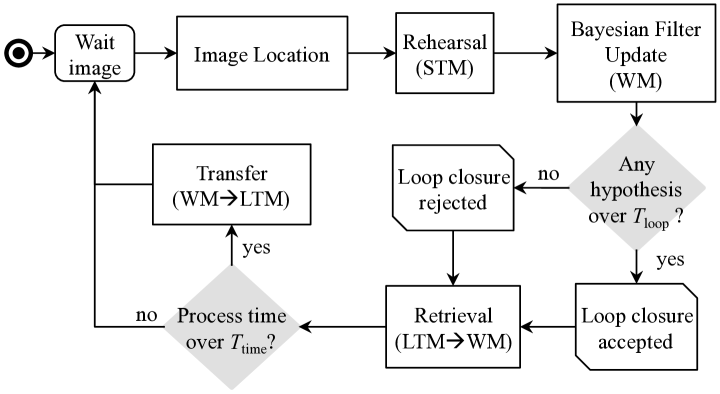
\includegraphics[width=0.9\textwidth]{figs/theory/rtabmap_memory_management.png}
    \caption{Flow chart of RTAB-Map memory management loop closure detection processing cycle.}
    \label{fig:rtabmap_memory_management}
\end{figure}

\subsection{Image Location}
\label{sec:image_location}
The bag-of-words approach \citep{sivic2003videogoogle} is used to create a signature $z_t$ of an image acquired at time $t$. An image signature is represented by a set of visual words contained in a visual dictionary incrementally constructed online using a randomized forest of kd-trees \citep{muja2009flann}. Speeded-Up Robust Features (SURF) \citep{bay2008surf} are extracted from the image as the visual words. A location $L_t$ is then created with signature $z_t$, a weight initialized to 0, and a bidirectional link in the graph with the previous location $L_{t-1}$. The dictionary contains only words of locations in \textbf{WM} and \textbf{STM}.

\subsection{Rehearsal}
\label{sec:rehearsal}
To update the weight of the acquired location, $L_t$ is compared to the ones in \textbf{STM} from the most recent ones to the latest, and similarity $\mathfrak{S}$ is evaluated using equation~(\ref{eq:similarity}):

\begin{equation}
    \label{eq:similarity}
    \mathfrak{S}(z_t, z_c) =
    \begin{cases}
        \dfrac{N_{\text{pair}}}{N_{z_t}}, & \text{if}\,\, N_{z_t} \ge N_{z_c} \\
        \dfrac{N_{\text{pair}}}{N_{z_c}}, & \text{if}\,\, N_{z_t} < N_{z_c}
    \end{cases}
\end{equation}
where $N_{\text{pair}}$ is the number of matched word pairs between the compared location signatures, and $N_{z_t}$ and $N_{z_c}$ are the total number of words of signature $z_t$ and the compared signature $z_c$ respectively. If $\mathfrak{S}(z_t, z_c)$ is higher than a fixed similarity threshold $T_{\text{rehearsal}}$, $L_c$ is merged into $L_t$ and Rehearsal stops. In Rehearsal, only words of $z_c$ are kept in the merged signature: $z_t$ is cleared and $z_c$ is copied into $z_t$. To complete the merging process, the weight of $L_t$ is increased by the one of $L_c$ plus one, the neighbor links of $L_c$ are added to $L_t$, and $L_c$ is deleted from \textbf{STM}.

\subsection{Bayesian Filter Update}
\label{sec:bayesian_filter_update}
The role of the discrete Bayesian filter is to keep track of loop closure hypotheses by estimating the probability that the current location $L_t$ matches one of the already visited locations stored in the \textbf{WM}. Let $S_t$ be a random variable representing the states of all loop closure hypotheses at time $t$. $S_t = i$ denotes the hypothesis that $L_t$ closes a loop with a past location $L_i$, thus detecting that $L_t$ and $L_i$ represent the same location. $S_t = -1$ denotes the hypothesis that $L_t$ is a new location. The filter estimates the full posterior probability $\mathbf{p}(S_t \mid L^t)$ for all $i = -1, \ldots, t_n$, where $t_n$ is the time index associated with the newest location in the \textbf{WM}, expressed by the following equation~(\ref{eq:bayesian_filter}):

\begin{equation}
        \label{eq:bayesian_filter}
        \mathbf{p}(S_t \mid L^t)
        = \eta\,\underbrace{\mathbf{p}(L_t \mid S_t)}_{\text{Observation}}
            \underbrace{\sum_{i=-1}^{t_n}
            \underbrace{\mathbf{p}(S_t \mid S_{t-1}=i)}_{\text{Transition}}\,\mathbf{p}(S_{t-1}=i \mid L^{t-1})}_{\text{Belief}}
\end{equation}
where $\eta$ is a normalization factor and $L^t$ is the set of all locations from $L_{-1}$ to $L_t$ in \textbf{WM} and \textbf{STM}, thus $L^t$ changes over time as new locations are added and when some locations are retrieved from \textbf{LTM} or transferred to \textbf{LTM}, deviating from the classical Bayesian filtering where such set is fixed. 
The observation model $\mathbf{p}(L_t \mid S_t)$ is evaluated using a likelihood function $\mathfrak{L}(S_t \mid L_t)$: the current location $L_t$ is compared using equation~(\ref{eq:similarity}) to locations corresponding to each loop closure state $S_t = j$ where $j = -1, \ldots, t_n$, giving a score $S_j = \mathfrak{S}(z_t, z_j)$. Each score is then normalized using the difference between the score $S_j$ and the standard deviation $\sigma$, normalized by the mean $\mu$ of all non-null scores, as in equation~(\ref{eq:likelihood})\citep{angeli2008fast}:
\begin{equation}
    \label{eq:likelihood}
    \mathbf{p}(L_t \mid S_t = j) = \mathfrak{L}(S_t = j \mid L_t) = 
    \begin{cases}
        \dfrac{S_j - \sigma}{\mu}, & \text{if}\,\, S_j \ge \mu + \sigma \\
        1, & \text{otherwise}.
    \end{cases}
\end{equation}
For the new location probability $S_t = -1$, the likelihood is evaluated using equation~(\ref{eq:likelihood2}):
\begin{equation}
    \label{eq:likelihood2}
    \mathbf{p}(L_t \mid S_t = -1) = \mathfrak{L}(S_t = -1 \mid L_t) = \dfrac{\mu}{\sigma} + 1
\end{equation}
where the score is relative to $\mu$ on $\sigma$ ratio. If $\mathfrak{L}(S_t = -1 \mid L_t)$ is high, meaning that $L_t$ is not similar to a particular one in \textbf{WM} (when $\sigma < \mu$), then $L_t$ is more likely to be a new location.
The transition model $\mathbf{p}(S_t \mid S_{t-1} = i)$ is used to predict the distribution of $S_t$, given each state of the distribution $S_{t-1}$ in accordance with the robot's motion between $t$ and $t-1$. Combined with $\mathbf{p}(S_{t-1} = i \mid L^{t-1})$ (i.e., the recursive part of the filter), this constitutes the belief of the next loop closure. The transition model is expressed as in \citep{angeli2008fast}.
\begin{itemize}
    \item $\mathbf{p}(S_t=-1 \mid S_{t-1}=-1) =0.9$, the probability of a new location event at time $t$ given that no loop closure occurred at time $t-1$.
    \item $\mathbf{p}(S_t=i \mid S_{t-1}=-1) = \frac{0.1}{N_{WM}}$ with $i \in [0, t_n]$, the probability of a loop closure event at time $t$ given that no loop closure occurred at time $t-1$. $N_{WM}$ is the number of locations in \textbf{WM} of the current iteration.

    \item $\mathbf{p}(S_t=-1 \mid S_{t-1}=j) = 0.1$ with $j \in [0, t_n]$, the probability of a new location event at time $t$ given that a loop closure occurred at time $t-1$ with $j$.
    \item $\mathbf{p}(S_t=i \mid S_{t-1}=j)$ with $i, j \in [0, t_n]$, the probability of a loop closure event at time $t$ given that a loop closure occurred at time $t-1$ on a neighbor location. The probability is defined as a discrete Gaussian curve centered on $j$ and where value are non-null for exactly eight neighbors $(for \,\, i=j-4, \ldots, j+4)$ and their sum are $0.9$.
\end{itemize}

\subsection{Loop Closure Hypothesis Selection}
\label{sec:loop_closure_hypothesis_selection}
When $\mathbf{p}(S_t \mid L^t)$ has been updated and normalized, highest hypothesis of $\mathbf{p}(S_t \mid L^t)$ greater than the loop closure threshold $T_{loop}$ is selected. Because a loop closure is generally diffused to its neighbors (neighbor locations share some similar words between them), for each probability $\mathbf{p}(S_t=i \mid L_t) \,\, where \,\, i \ge 0$, the probablilities of its neighbors in the range defined by the transition model $\mathbf{p}(S_t=i \mid S_{t-1}=j)$ are summed together. Note that for a selection to occur, aminimum of $T_{minHyp}$ locations must be in \textbf{WM}: when the graph is initialized, the first locations added to \textbf{WM} have automatically a high loop closure probability (after normalization by the equation~(\ref{eq:bayesian_filter})), therefore wrong loop closures could be accepted if the hypothesis are over $T_{loop}$.

If there is loop closure hypothesis $\mathbf{p}(S_t=i \mid L^t) \,\, where \,\, i \ge 0$ is over $T_{loop}$, the hypothesis $S_t=i$ is then accepted, $L_t$ is merged with the old location $L_i$: the weight of $L_t$ is increased by the one of $L_i$ plus one and the neighbor links of $L_i$ are added to $L_t$. After updatoing $L_t$, unlike \textbf{Rehearsal}, $L_i$ is not deleted from \textbf{WM}. For the constancy of the Bayesian filter with the next acquired images, the associated loop closure hypothesis $S_i$ must be evaluated until $L_i$ is not anymore in the neighborhood of the highest loop closure hypothesis, after which it is removed. 

\subsection{Retrieval}
\label{sec:retrieval}
Neighbors of location $L_i$ in \textbf{LTM} are transferred back into \textbf{WM} if $\mathbf{p}(S_t=i \mid L^t)$ is the heighest probability. Because this step is time consuming, a maximum of two locations are retrived at each iteration (choosen inside the neighboring range defined in Section~\ref{sec:bayesian_filter_update}). The visual dictionary is updated with the words associated with the signatures of the retrieved locations. Common words from the retrieved signatures still exist in the dictionary, so a simple reference is added between these words and the corresponding signatures. For words that are not present anymore (because they were removed from the dictionary when the locations were transferred), they are matched to those in the dictionary to find if more recent words represent the same \textbf{SURF} features. This step is particularly important because the new words added from the new signature $z_t$ may be identical to the previously transferred words. For matched words, the old words are replaced by the new ones in the retrieved signatures. All the references in the \textbf{LTM} are changed and the old words are permanently removed. If some words are still unmatched, they are simply added to the dictionary.

\subsection{Transfer}
When processing time becomes greater than $T_{time}$, the oldest location with the lowest weight is transferred from \textbf{WM} to \textbf{LTM}. $T_{time}$ must be set to allow the robot to process the perceived images in real-time. Higher $T_{time}$ means that more locations (and implicitly more words) can be kept in the \textbf{WM}, and more loop closure hypotheses can be kept to better represent the overall environment. $T_{time}$ must therefore be set according to the robot's CPU capabilities, computational load and operating environmetn. If $T_{time}$ is set to higher than the image acquisition time, the algorithm intrinsically uses an image rate corresponding to $T_{time}$, with 100\% CPU usage. As a rule of thumb, $T_{time}$ can be set to about 200 to 400 ms smaller to the image acquisition rate at 1 Hz, to ensure that all images are processed under the image acquisition rate, even if the processing time goes over $T_{time}$. ($T_{time}$ then corresponds to the average processing time of an image by the algorithm). So, for an image acquisition rate of 1 Hz, $T_{time}$ can be set to between 600 and 800 ms.

Because the most expensive step of the algorithm is to rebuild the visual dictionary, process time can be regulated by changing the dictionary size, which indirectly influences the \textbf{WM} size. A signature of a location transferred to \textbf{LTM} removes its word references from the visual dictionary. If a word does not have reference to a signature anymore, it is transferred into \textbf{LTM}. While the number of words transferred from the dictionary is less than the number of words added from the new or retrieved locations, more locations are transferred. At the end of this process, the dictionary size is smaller than before the new words from the new and retrieved locations were added, thus reducing the time required to update the dictionary for the next acquired image. Saving the transferred locations into the database is done asynchronously using a background thread, leading to a minimal time overhead. Note also that to be able to evaluate appropriately loop closure hypotheses using the discrete Bayesian filter, the retrieved locations of the current iteration are not allowed to be transferred.

\section{ROS2 Working Framework\label{sec:ros2_working_framework}}
% 中文版：
% \section{ROS2工作框架\label{sec:ros2_working_framework}}
% 本工程的另一个理论基础是ROS2（Robot Operating System 2）工作框架。ROS2是一个开源的机器人操作系统，它提供了一种灵活的框架，用于编写机器人软件。ROS2的工作框架包括多个核心概念和组件，这些概念和组件共同协助开发者构建功能丰富的机器人应用程序。为帮助读者更好地理解本文，在这里对ROS2的一些核心概念和组件进行简要介绍，如需了解更多内容，请参考相关文献\citep{ros2humble}。

% 以下是ROS2工作框架的主要组成部分：
% \begin{itemize}
%     \item \textbf{节点（Nodes）}：ROS2中的节点是独立的进程，
%     每个节点可以执行特定的任务。节点之间通过消息传递进行通信。
%     \item \textbf{主题（Topics）}：主题是节点之间传递消息的通道。
%     节点可以发布消息到主题上，其他节点可以订阅这些主题以接收消息。
%     \item \textbf{服务（Services）}：服务提供了一种请求-响应的通信方式
%     ，允许一个节点请求另一个节点执行某个操作并返回结果。
%     \item \textbf{动作（Actions）}：动作是一种更复杂的通信方式，
%     允许节点执行长时间运行的任务，并提供反馈和结果。
%     \item \textbf{参数（Parameters）}：参数允许节点在运行时配置其行为。
%     节点可以读取和设置参数，以便在运行时调整其功能。
%     \item \textbf{坐标转换（Transformations）}：ROS2提供了坐标转换功能，
%     允许节点在不同坐标系之间进行转换。这对于处理传感器数据和机器人运动非常重要。
%     \item \textbf{分布式系统（Distributed System）}：ROS2支持分布式系统，
%     允许多个节点在不同的计算机上运行并协同工作。
%     这使得机器人系统可以扩展到更复杂的应用场景。
%     \item \textbf{中间件（Middleware）}：当多个节点部署到不同的计算机上时，
%     ROS2使用中间件Data-Distribution Service（DDS）来处理节点之间的通信。
% \end{itemize}

% English version:
The ROS2 (Robot Operating System 2) working framework is another theoretical foundation of this engineering project. ROS2 is an open-source robot operating system that provides a flexible framework for writing robot software. The ROS2 working framework includes some core concepts and components that work together to assist developers in building feature-rich robotic applications. To help readers better understand this project, a brief introduction to some core concepts and components of ROS2 is provided here. For more information, please refer to the relevant literature \citep{ros2humble}.

\subsection{ROS graph}
\label{sec:ros2_graph}
The ROS graph is a network of ROS 2 elements processing data together at the same time. It encompasses all executables and the connections between them if you were to map them all out and visualize them. Appendix~\ref{app:ros2graphs} provides ROS2 graphs from different stages of this engineering project, showing how the ROS2 graph evolves as the engineering progresses.

\subsection{Node}
\label{sec:ros2_node}
Each node in ROS should be responsible for a single, modular purpose, e.g. controlling the wheel motors or publishing the sensor data from a laser range-finder. As shown in Figure~\ref{fig:ros2_nodes}, each node can send and receive data from other nodes via topics, services, actions, or parameters.
\begin{figure}[htbp] 
    \centering 
    \begin{subfigure}[t]{0.9\textwidth} 
        \centering 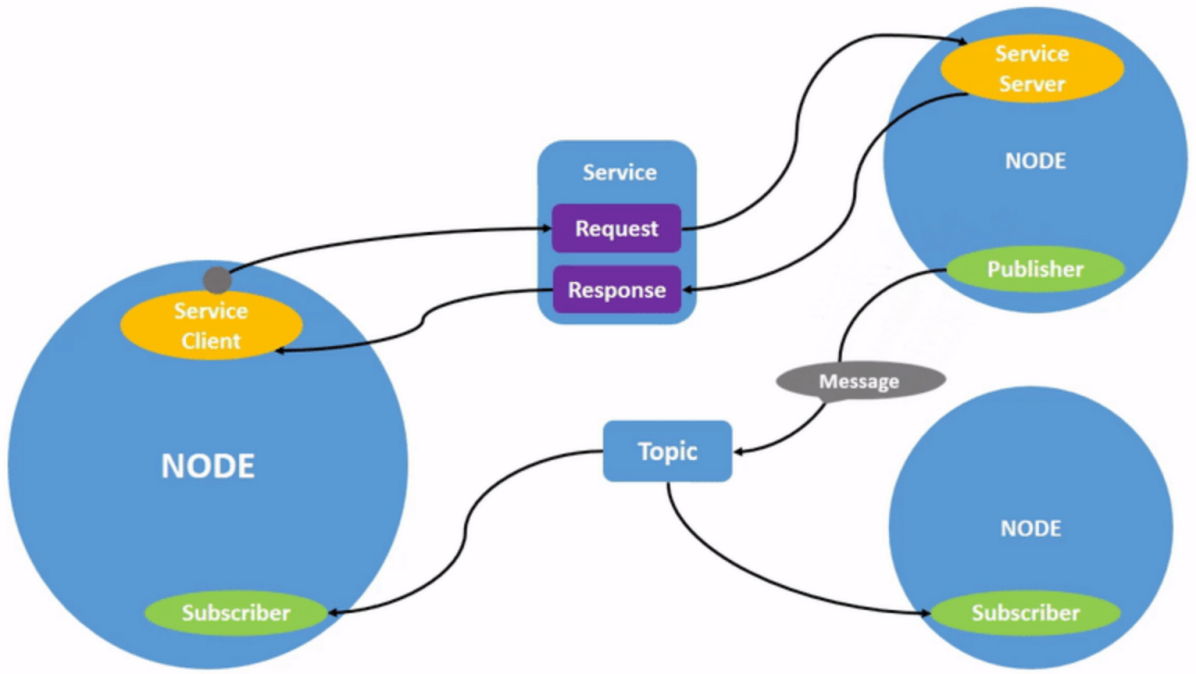
\includegraphics[width=\linewidth]{figs/theory/ros2_node2_01.png} 
        \subcaption{Publish message} \label{fig:ros2_node2:Publisher} 
    \end{subfigure} 
    \vspace{0.5cm}
    \begin{subfigure}[t]{0.9\textwidth} 
        \centering 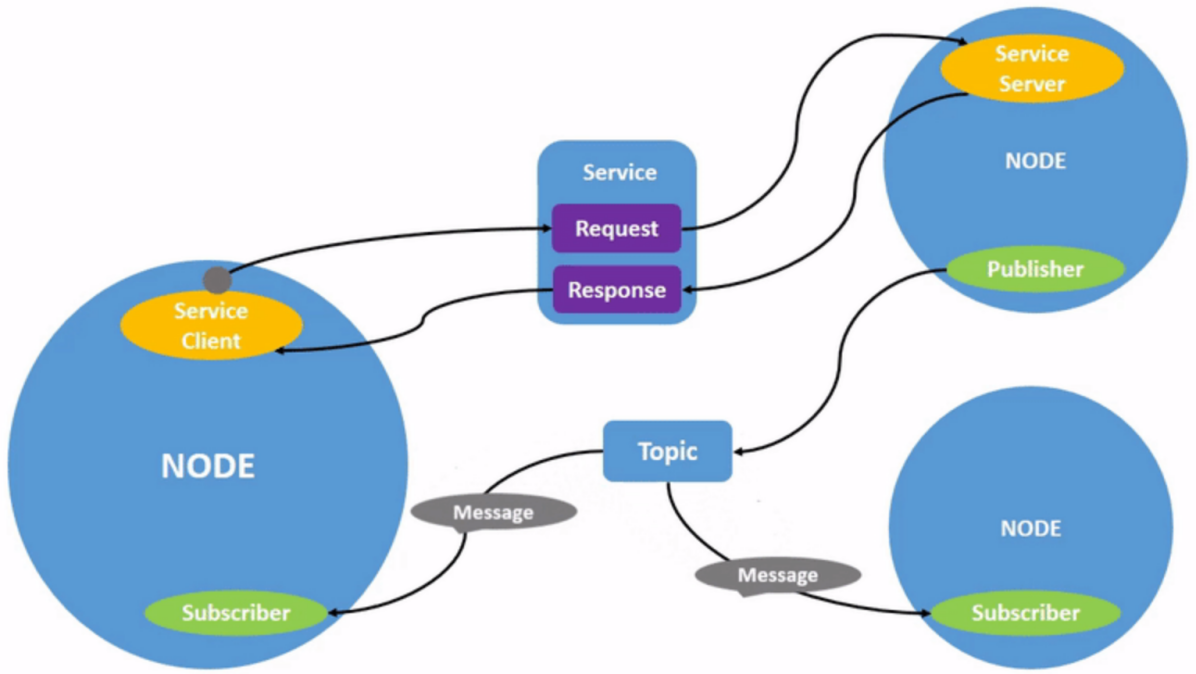
\includegraphics[width=\linewidth]{figs/theory/ros2_node2_02.png} 
        \subcaption{Subscribe messages} \label{fig:ros2_node2:Subscribers} 
    \end{subfigure} 
    \caption{ROS2 Nodes (Publisher) \& (Subscribers)} 
    \label{fig:ros2_nodes} 
\end{figure}

A full robotic system is comprised of many nodes working in concert. In ROS 2, a single executable (C++ program, Python program, etc.) can contain one or more nodes. A node is a fundamental ROS 2 element that serves a single, modular purpose in a robotics system.

\subsection{Topic}
\label{sec:ros2_topic}
ROS 2 breaks complex systems down into many modular nodes. Topics are a vital element of the ROS graph that act as a bus for nodes to exchange messages. As shown in Figure~\ref{fig:ros2_topics}, nodes can publish messages to a topic, and other nodes can subscribe to that topic to receive those messages. This allows for a flexible and decoupled communication mechanism between nodes. A node may publish data to any number of topics and simultaneously have subscriptions to any number of topics.
Topics are one of the main ways in which data is moved between nodes and therefore between different parts of the system.

\begin{figure}[htbp] 
    \centering 
    \begin{subfigure}[t]{0.9\textwidth} 
        \centering 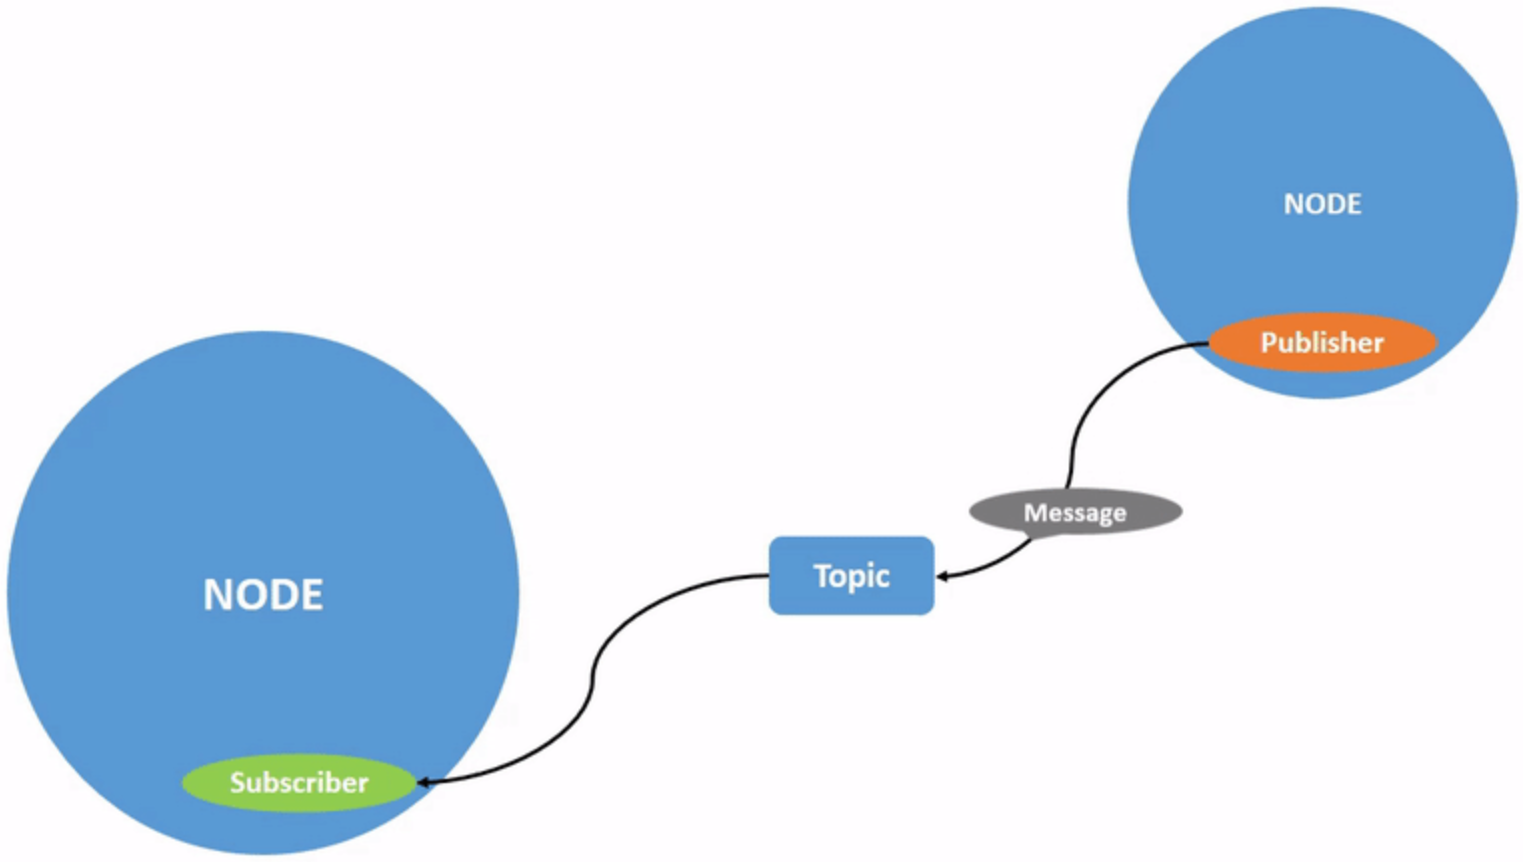
\includegraphics[width=\linewidth]{figs/theory/ros2_topic_01.png} 
        \subcaption{one-to-one} \label{fig:ros2_node2_one2one} 
    \end{subfigure} 
    \vspace{0.5cm}
    \begin{subfigure}[t]{0.9\textwidth} 
        \centering 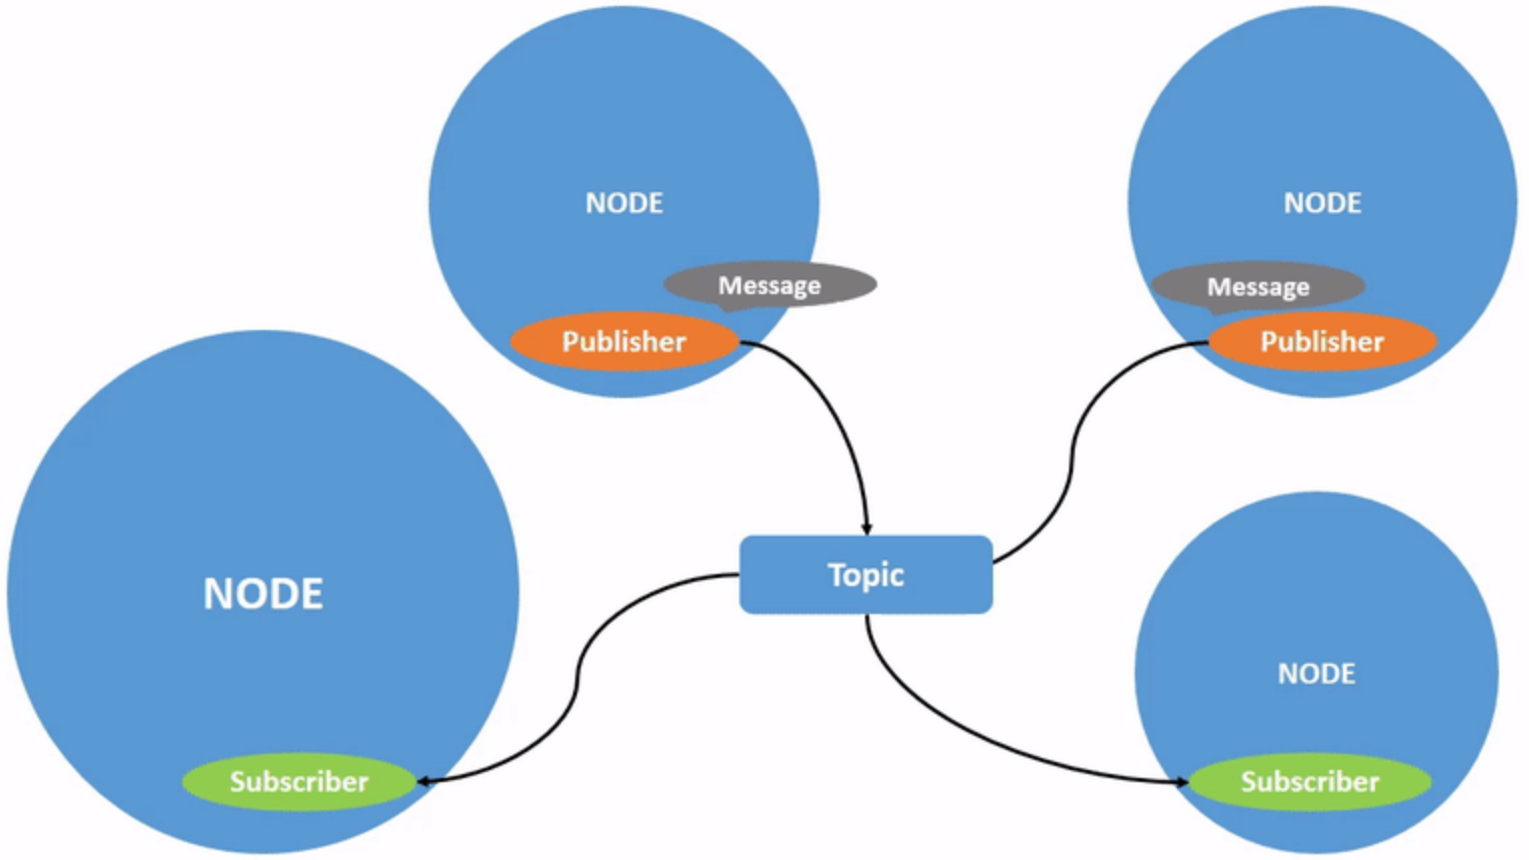
\includegraphics[width=\linewidth]{figs/theory/ros2_topic_02.png} 
        \subcaption{many to many} \label{fig:ros2_node2_many2many} 
    \end{subfigure} 
    \caption{ROS2 Topics (one-to-one) \& (many to many)} 
    \label{fig:ros2_topics} 
\end{figure}

\subsection{Service}
\label{sec:ros2_service}
Services are another method of communication for nodes in the ROS graph. Services are based on a call-and-response model versus the publisher-subscriber model of topics. While topics allow nodes to subscribe to data streams and get continual updates, services only provide data when they are specifically called by a client.
\begin{figure}[htbp] 
    \centering 
    \begin{subfigure}[t]{0.9\textwidth} 
        \centering 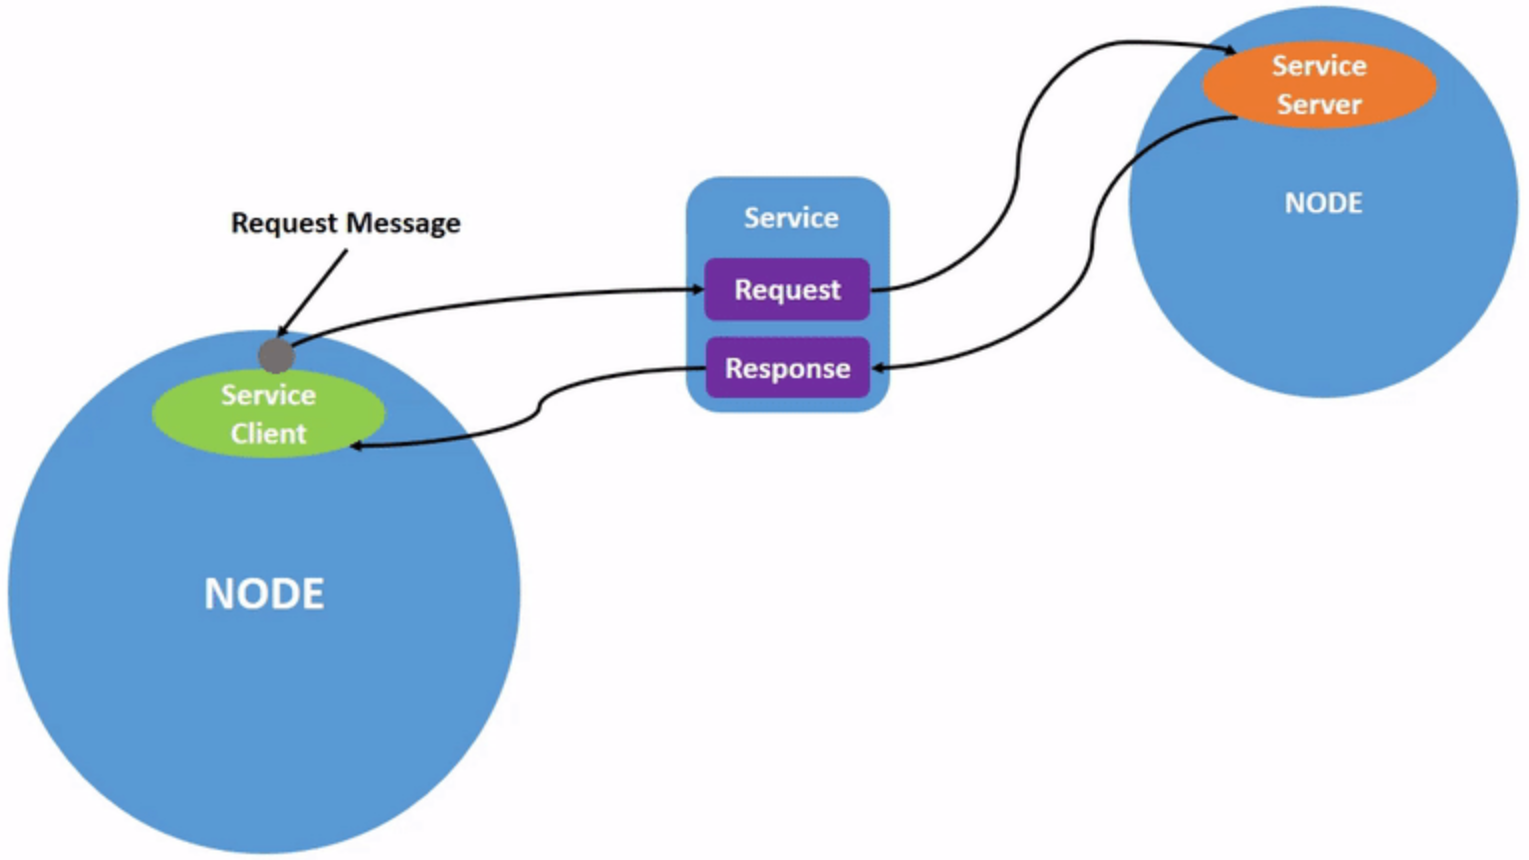
\includegraphics[width=\linewidth]{figs/theory/ros2_service_01.png} 
        \subcaption{one-to-one} \label{fig:ros2_service_one2one} 
    \end{subfigure} 
    \vspace{0.5cm}
    \begin{subfigure}[t]{0.9\textwidth} 
        \centering 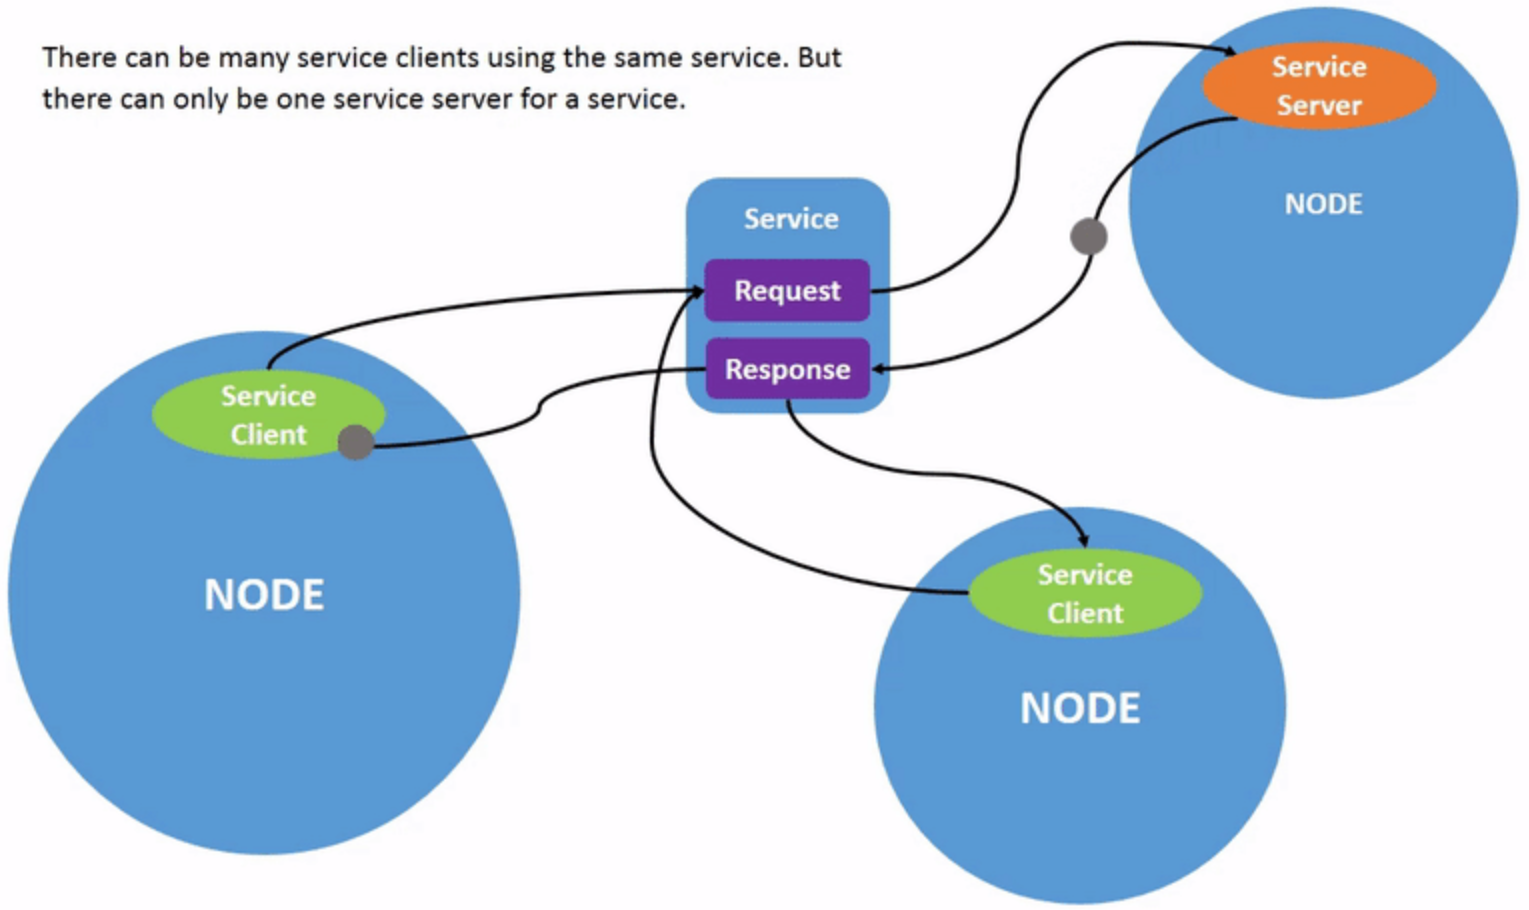
\includegraphics[width=\linewidth]{figs/theory/ros2_service_02.png} 
        \subcaption{many to one} \label{fig:ros2_node2_many2one} 
    \end{subfigure} 
    \caption{ROS2 Services (one-to-one) \& (many to one)} 
    \label{fig:ros2_services} 
\end{figure}
Nodes can communicate using services in ROS 2. Unlike a topic - a one way communication pattern where a node publishes information that can be consumed by one or more subscribers - a service is a request/response pattern where a client makes a request to a node providing the service and the service processes the request and generates a response.

\subsection{Action}
Actions are one of the communication types in ROS 2 and are intended for long running tasks. They consist of three parts: a goal, feedback, and a result.

As shown in Figure~\ref{fig:ros2_action}, actions are built on topics and services. Their functionality is similar to services, except actions can be canceled. They also provide steady feedback, as opposed to services which return a single response. 

Actions use a client-server model, similar to the publisher-subscriber model (described in the section~\ref{sec:ros2_topic}). An “action client” node sends a goal to an “action server” node that acknowledges the goal and returns a stream of feedback and a result.

\begin{figure}[htbp]
    \centering
    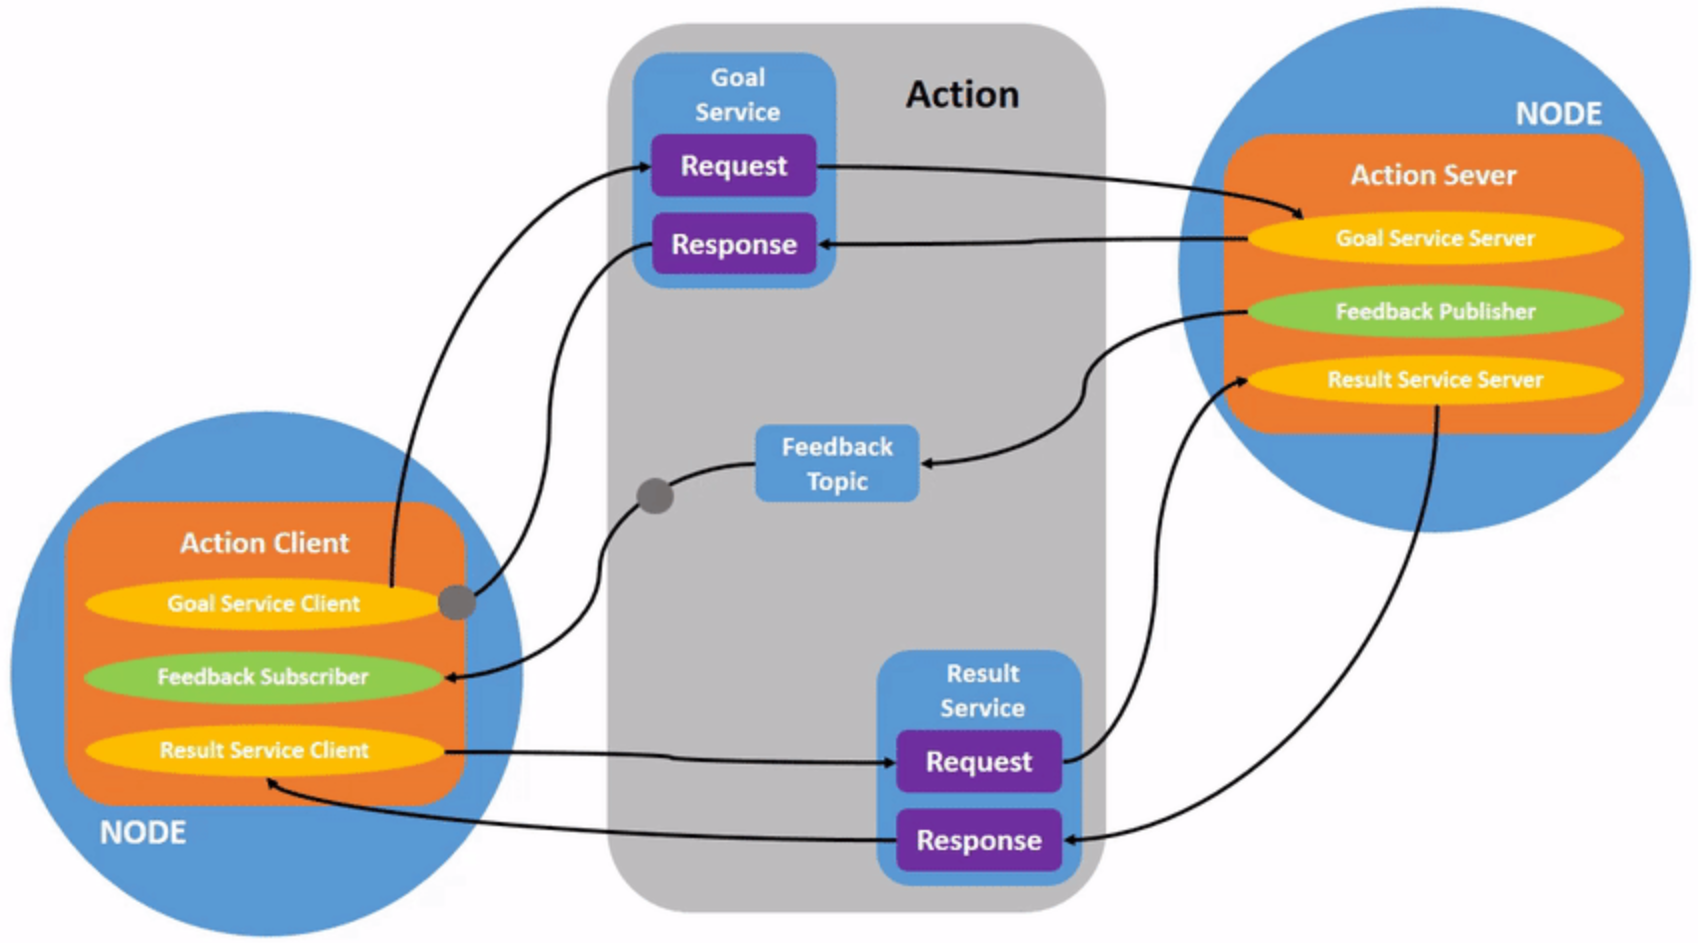
\includegraphics[width=0.9\textwidth]{figs/theory/ros2_action.png}
    \caption{ROS2 Action}
    \label{fig:ros2_action}
\end{figure}

A robot system would likely use actions for navigation. An action goal could tell a robot to travel to a position. While the robot navigates to the position, it can send updates along the way (i.e. feedback), and then a final result message once it’s reached its destination.

\subsection{Parameter}
\label{sec:ros2_parameter}
A parameter is a configuration value of a node. You can think of parameters as node settings. A node can store parameters as integers, floats, booleans, strings, and lists. In ROS 2, each node maintains its own parameters.

Nodes have parameters to define their default configuration values. You can get and set parameter values from the command line. You can also save the parameter settings to a file to reload them in a future session.

\subsection{TF2}
\label{sec:ros2_transform}
tf2 is the second generation of the transform library, which lets the user keep track of multiple coordinate frames over time. tf2 maintains the relationship between coordinate frames in a tree structure buffered in time, and lets the user transform points, vectors, etc between any two coordinate frames at any desired point in time.

Figure~\ref{fig:tf2_vslam_tree} shows the tf2 tree structure used in this engineering project. The root frame is the \texttt{map} frame, which is the global coordinate frame of the environment. The \texttt{odom} frame is the odometry frame, which is used to track the robot's position and orientation over time. The \texttt{zed\_camera\_link} frame is the robot's base frame, which is used to represent the robot's position and orientation in the environment. The \texttt{zed\_left\_camera\_frame} and \texttt{zed\_right\_camera\_frame} frames are the left and right camera frames, respectively, which are used to represent the stereo camera's position and orientation.

\begin{figure}[htbp]
    \centering
    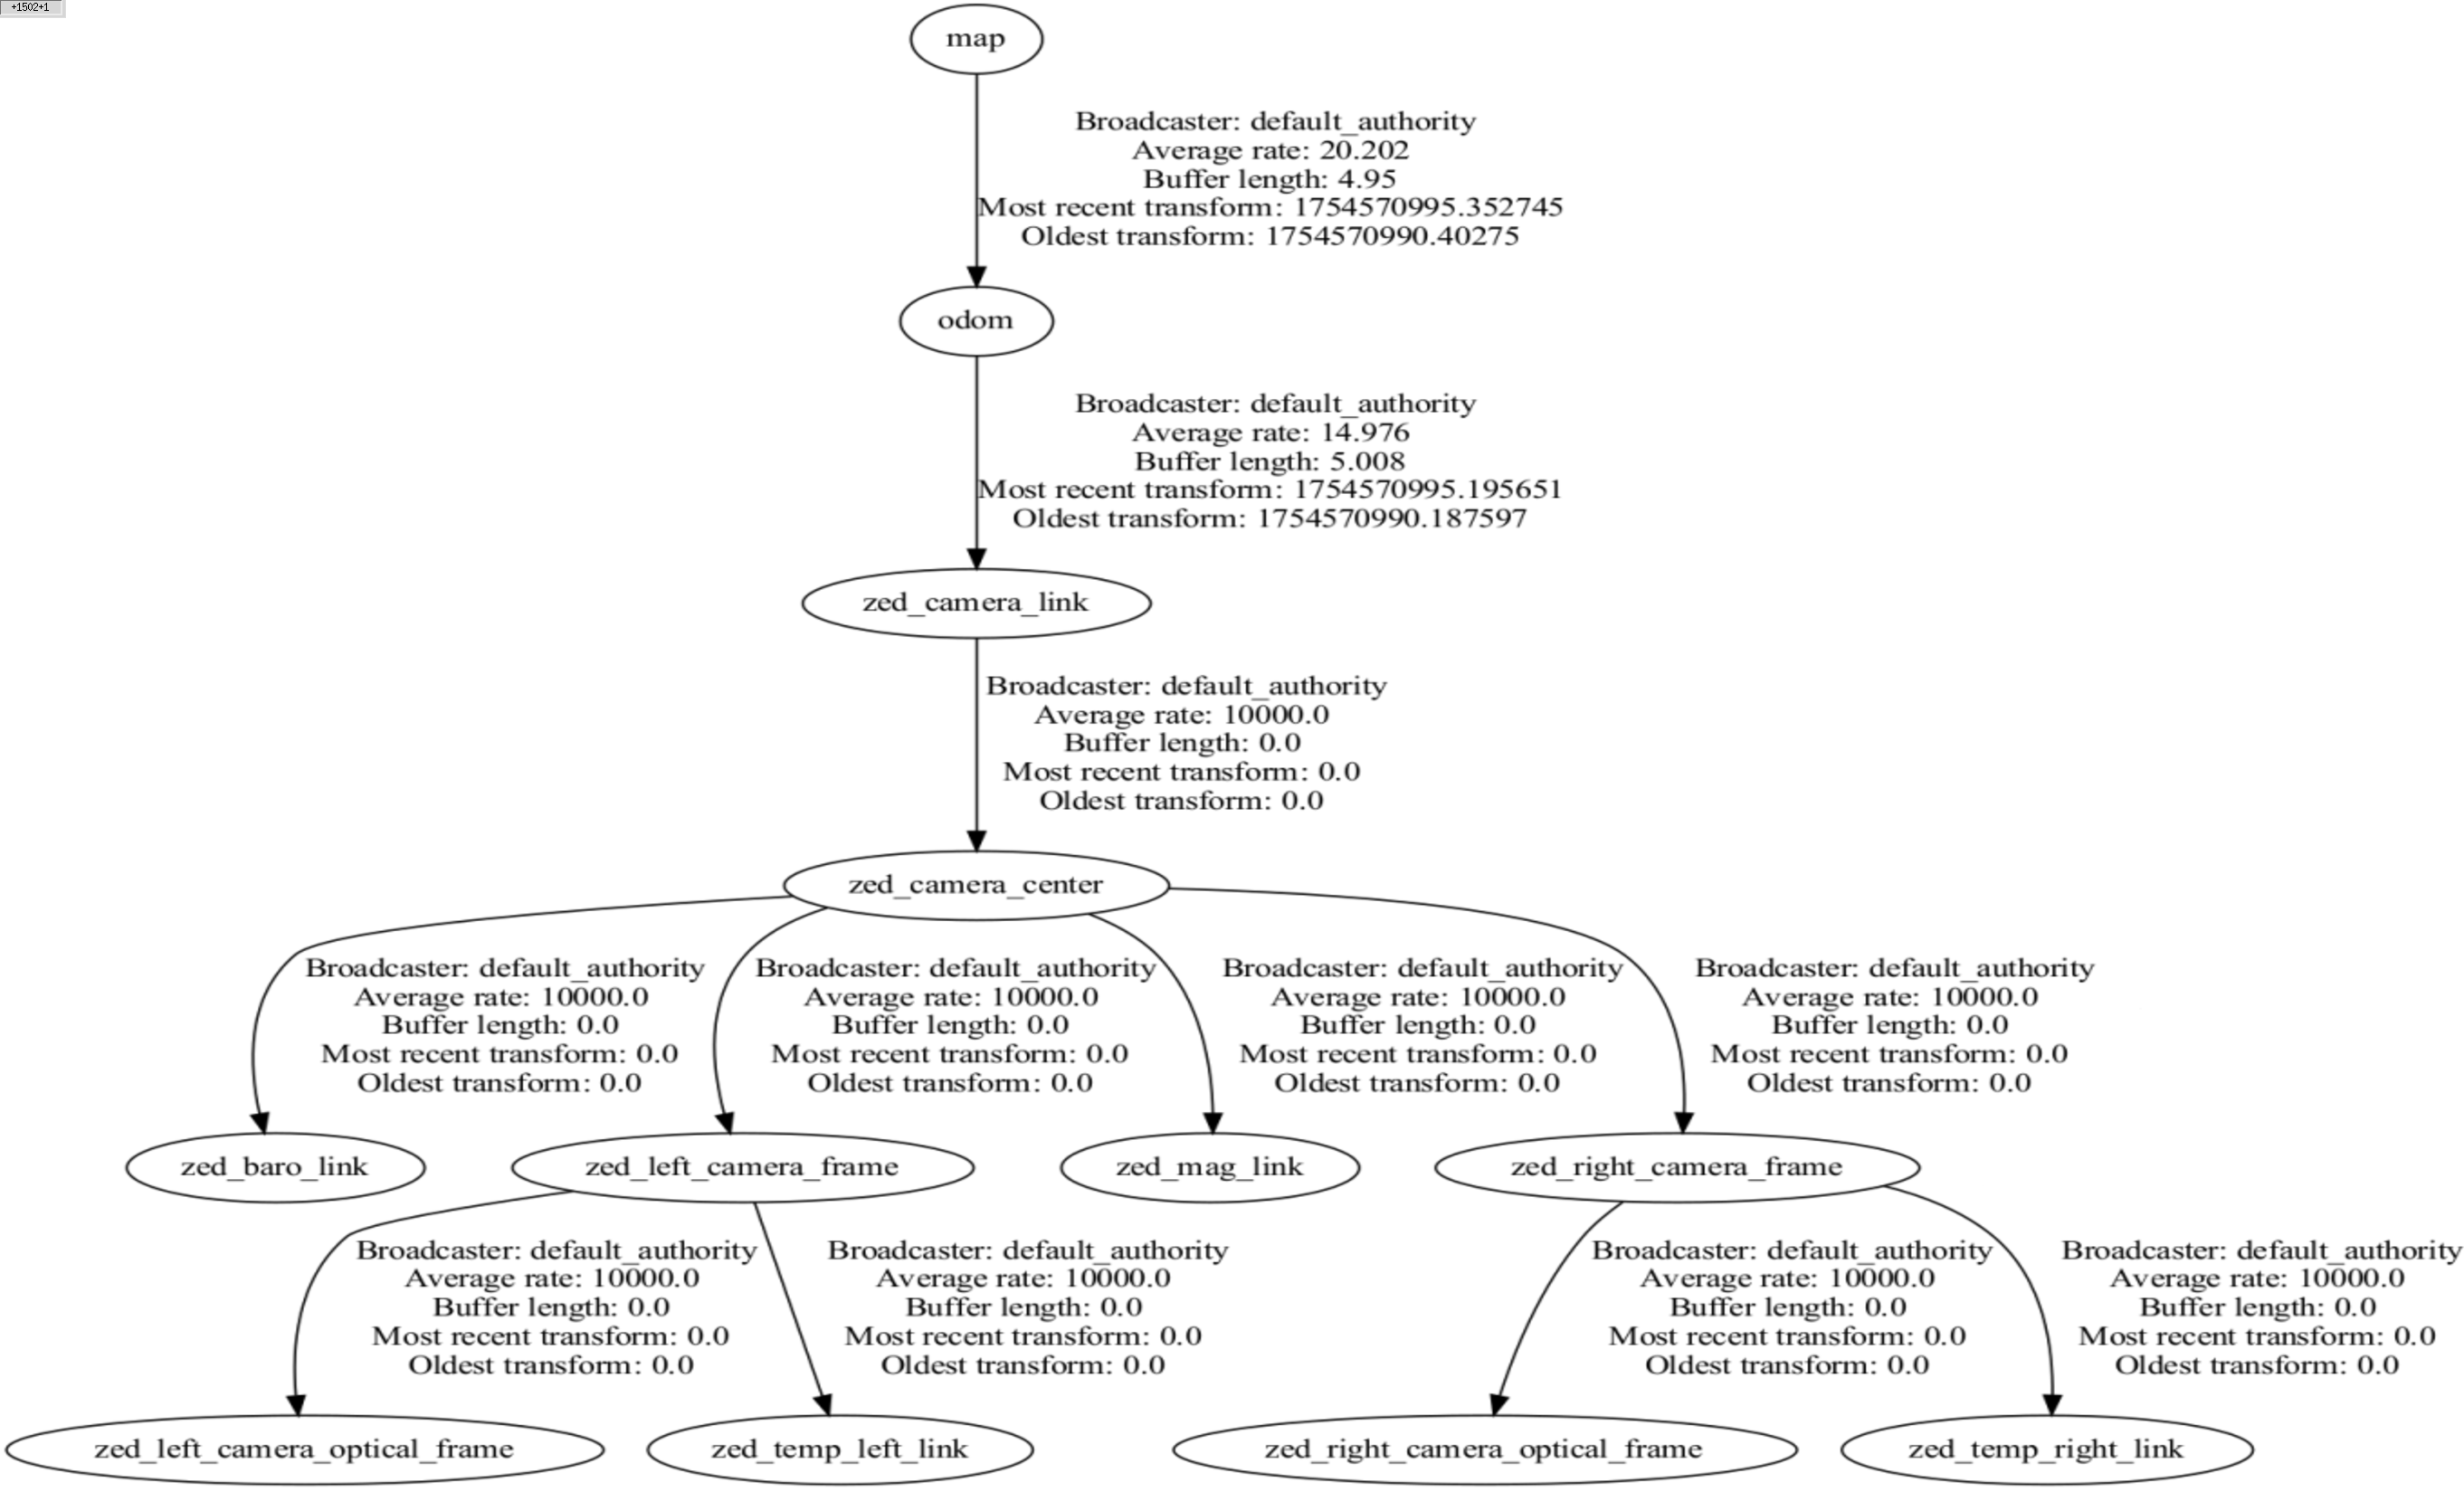
\includegraphics[width=0.9\textwidth]{figs/theory/tf2_vslam_tree.png}
    \caption{TF2 tree structure used in this engineering project.}
    \label{fig:tf2_vslam_tree}
\end{figure}


\chapter{Engineering Design\label{chap:design}}
% 中文版：
% 本章将对该工程的系统架构进行详细阐述，系统总架构如图Figure~\ref{fig:overall_architecture}所示。

%接下来将针对建图架构、定位架构、无人机递送架构、导航架构等部分进行分别介绍。

% English Version：
This chapter will provide a description of the system design for the engineering, including use case, architecture and data flow. Next, we will introduce them one by one.

\section{Use Case}
First of all, we will introduce the use case of the engineering. The use case is shown in Figure~\ref{fig:use_case}.
\begin{figure}[h]
    \centering
    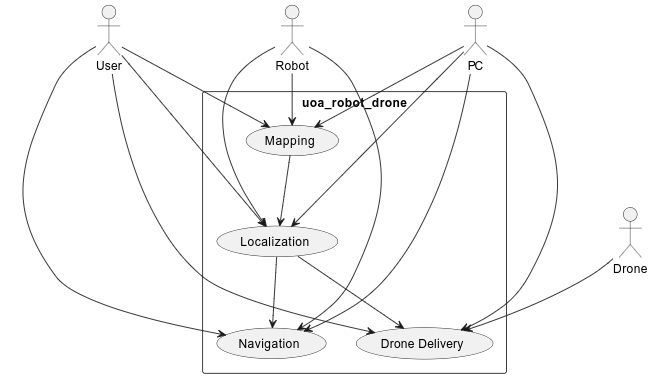
\includegraphics[width=0.9\textwidth]{figs/uml/use_case.png}
    \caption{Use Case}
    \label{fig:use_case}
\end{figure}
There are four actors in the use case:
\begin{itemize}
    \item \textbf{User}: The user can control the robot to move around, set a target position, and monitor the robot's status.
    \item \textbf{Robot}: The robot can perform mapping, localization, and navigation tasks, and can also deliver items using a drone.
    \item \textbf{Drone}: The drone can be controlled by the robot to deliver items to a specified target position.
    \item \textbf{PC}: The PC is a personal computer that runs the uoa\_robot\_drone engineering package, which includes nodes for monitoring the robot's status and controlling the drone.
\end{itemize}
There are four main use cases in the use case diagram:
\begin{itemize}
    \item \textbf{Mapping}: The robot can perform mapping tasks to create a map of the environment.
    \item \textbf{Localization}: The robot can determine its position in the environment using the map created during the mapping stage.
    \item \textbf{Drone Delivery}: The robot can control the drone to deliver items to a specified target position.
    \item \textbf{Navigation}: The robot can navigate to a specified target position using the map created during the mapping stage and the localization information. 
\end{itemize}
The following section is Engineering System Architecture.

\section{Engineering System Architecture}
This distributed system architecture consists of three main components: Raspberry Pi, Jetson Orin Nano, and Personal Computer. Each component integrates multiple hardware and software modules, as shown in Figure~\ref{fig:system_architecture}, to collaboratively accomplish mapping, localization, navigation, and drone delivery tasks.
\begin{figure}[htbp]
    \centering
    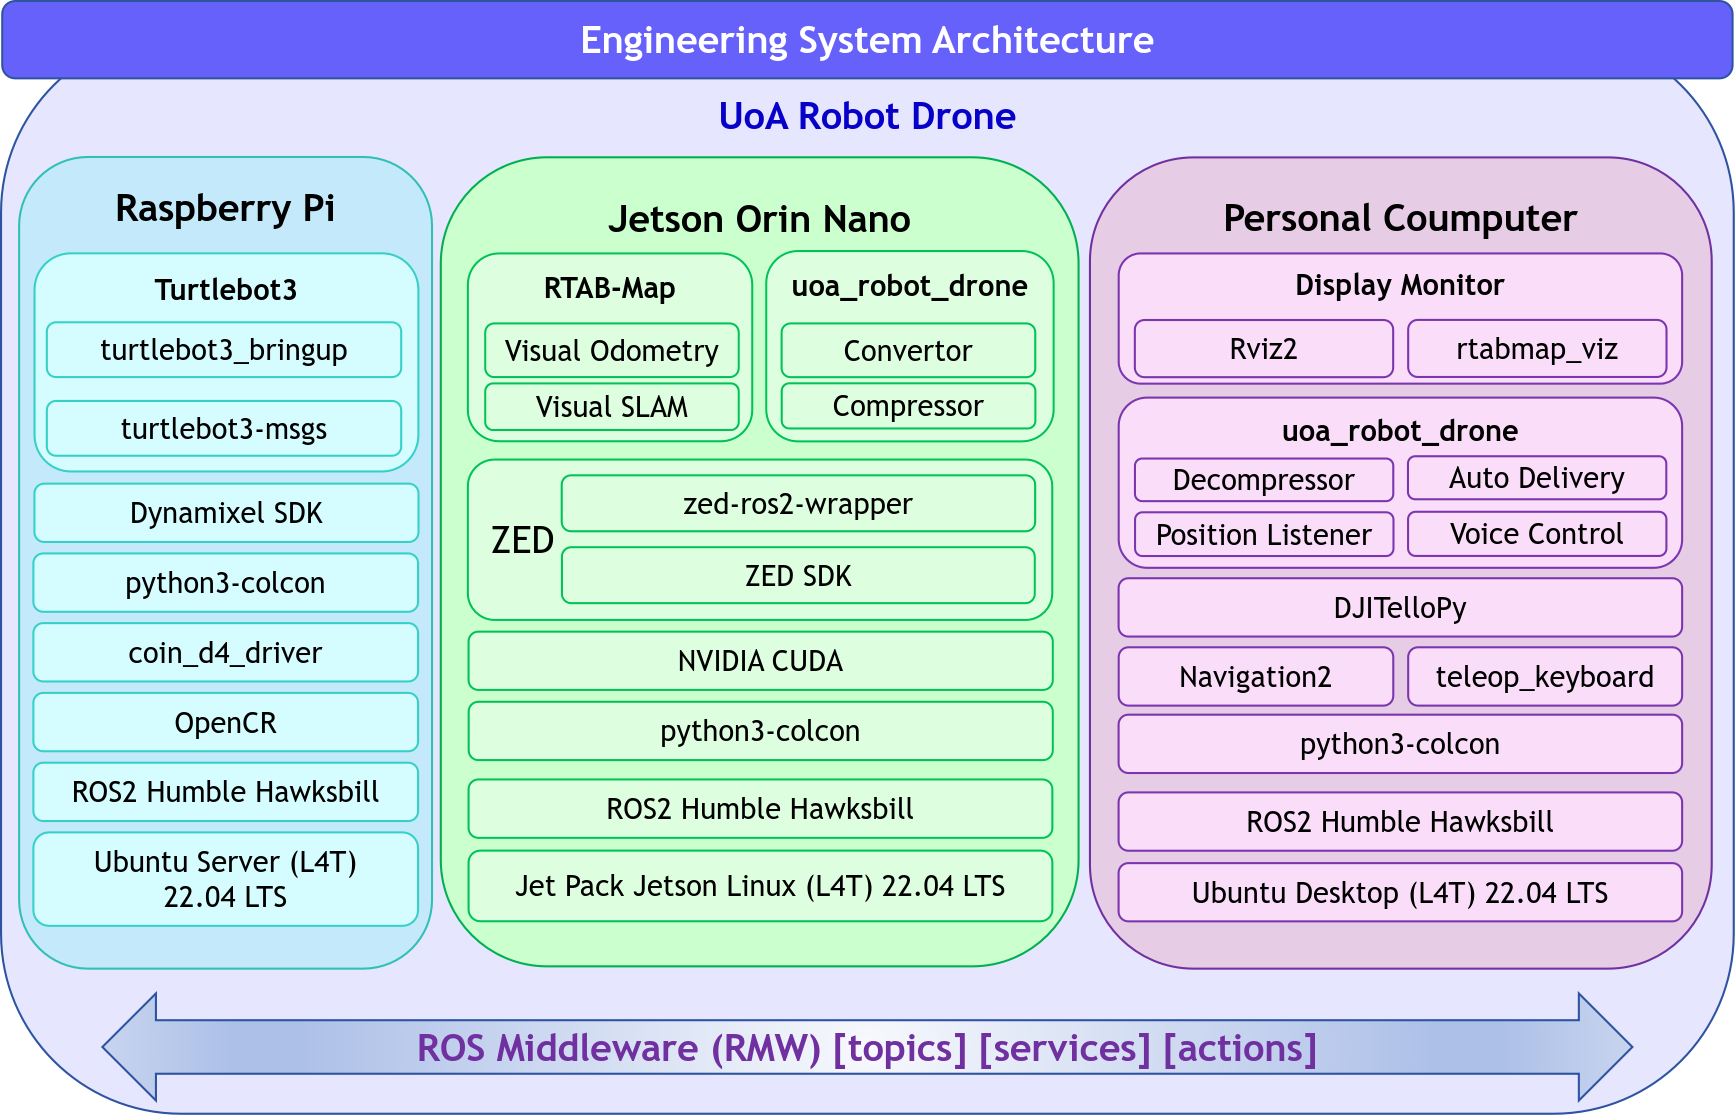
\includegraphics[width=0.9\textwidth]{figs/architecture/architecture.png}
    \caption{Engineering System Architecture}
    \label{fig:system_architecture}
\end{figure}

\begin{itemize}
    \item \textbf{Raspberry Pi}:
    \begin{itemize}
        \item \textbf{Turtlebot3}:
        \begin{itemize}
            \item \texttt{turtlebot3\_bringup}: Launches core robot nodes and drivers.
            \item \texttt{turtlebot3-msgs}: Defines message types for robot communication.
        \end{itemize}
        \item \texttt{Dynamixel SDK}: Motor control library for actuators.
        \item \texttt{python3-colcon}: ROS2 build and package management tool.
        \item \texttt{coin\_d4\_driver}: Driver for additional hardware components.
        \item \texttt{OpenCR}: Controller board for sensors and actuators.
        \item \texttt{ROS2 Humble Hawksbill}: Robot Operating System for distributed communication.
        \item \texttt{Ubuntu Server (L4T) 22.04 LTS}: Operating system for the Raspberry Pi.
    \end{itemize}

    \item \textbf{Jetson Orin Nano}:
    \begin{itemize}
        \item \textbf{RTAB-Map}:
        \begin{itemize}
            \item Visual Odometry: Estimates robot motion from camera data.
            \item Visual SLAM: Simultaneous localization and mapping.
        \end{itemize}
        \item \textbf{uoa\_robot\_drone}:
        \begin{itemize}
            \item Convertor: Image format conversion ($bgra8 \rightarrow bgr8$) for efficient processing.
            \item Compressor: Compresses image data for transmission.
        \end{itemize}
        \item \textbf{ZED}:
        \begin{itemize}
            \item \texttt{zed-ros2-wrapper}: ROS2 interface for ZED stereo camera.
            \item \texttt{ZED SDK}: Provides stereo vision and depth data.
        \end{itemize}
        \item \texttt{NVIDIA CUDA}: GPU acceleration for vision algorithms.
        \item \texttt{python3-colcon}, \texttt{ROS2 Humble Hawksbill}: As above.
        \item \texttt{Jet Pack Jetson Linux (L4T) 22.04 LTS}: Operating system for Jetson Orin Nano.
    \end{itemize}

    \item \textbf{Personal Computer}:
    \begin{itemize}
        \item \textbf{Display Monitor}:
        \begin{itemize}
            \item \texttt{Rviz2}: Visualization of robot state and environment.
            \item \texttt{rtabmap\_viz}: SLAM and mapping visualization.
        \end{itemize}
        \item \textbf{uoa\_robot\_drone}:
        \begin{itemize}
            \item Decompressor: Decompresses image data from Jetson.
            \item Auto Delivery: Controls drone delivery tasks.
            \item Position Listener: Monitors robot/drone position.
            \item Voice Control: Enables voice command interface.
        \end{itemize}
        \item \texttt{DJITelloPy}: Python library for controlling DJI Tello drone.
        \item \texttt{Navigation2}: Path planning and autonomous navigation.
        \item \texttt{teleop\_keyboard}: Manual robot control via keyboard.
        \item \texttt{python3-colcon}, \texttt{ROS2 Humble Hawksbill}: As above.
        \item \texttt{Ubuntu Desktop (L4T) 22.04 LTS}: Operating system for the PC.
    \end{itemize}
\end{itemize}

All modules communicate via ROS2 middleware (topics, services, actions), enabling seamless data exchange and coordinated operation across the distributed system.


% The next section will introduce the module sequence of each use case.

% \section{Module Sequence}
% This section will state four module sequences for the use cases of mapping, localization, drone delivery, and navigation. 
% \subsection{Mapping Module Sequence}
% The mapping module sequence is shown in Figure~\ref{fig:mapping_sequence}.
% \begin{figure}[htbp]
%     \centering
%     \includegraphics[width=0.9\textwidth]{figs/uml/mapping_sequence.png}
%     \caption{Mapping Module Sequence}
%     \label{fig:mapping_sequence}
% \end{figure}

The next section will introduce the \textbf{Data Flow} of the engineering system.

\section{Data Flow}
The data flow is shown in Figure~\ref{fig:data_flow}.

\begin{figure}[htbp]
    \centering
    
\includegraphics[width=0.9\textwidth]{figs/architecture/data_flow.png}
    \caption{Data Flow}
    \label{fig:data_flow}
\end{figure}

% 中文版：
% \begin{itemize}
% Figure~\ref{fig:data_flow}中图例解释：
%   \item 椭圆形：表示工作包或节点(teleop_keyboard,rtabmap_viz, rviz2代表节点，其它为工作包)
%   \item 嵌套圆角矩形: \\
%       * 外层表示工作包 \\
%       * 内层表示launch文件 \\
%   \item 直角矩形：\\
%       * 以"/"开头的表示ROS话题
%       * 以字母开头的表示数据
%   \item 箭头：表示数据流向，其中：
%       * 实线箭头表示一直存在的数据流向
%       * 虚线箭头表示数据流向在某些阶段才存在，如rtabmap包中的/map话题在建图阶段存在，导航阶段不存在，由navigation2包中的/map_server节点发布的/map话题在导航阶段存在，建图阶段不存在。
%   \item 圆柱形：表示数据存储
%   \item 尖圆型：表示地图数据
%   \item TF：表示坐标变换
% \end{itemize}
% 具体数据流如下：
% \subsection{立体相机获取左右摄像头图像数据}
% 摄像头获取外界图像数据后，会通过/zed/zed_node节点发布两类四个话题的图像数据：
% camera_info类话题：发布相机的内参和外参信息，包含相机的焦距、畸变系数等参数。发布的两个话题名称分别为：
% \begin{itemize}
%     \item /zed2/zed_node/left/camera_info
%     \item /zed2/zed_node/right/camera_info
% \end{itemize}
% camera类的这两个话题数据可以直接向下传递给rtabmap节点进行使用。
% image矫正后的图像类话题：发布矫正后的左右图像数据，包含图像的宽度、高度、编码格式等信息。发布的两个话题名称分别为：
% \begin{itemize}
%     \item /zed2/zed_node/left/image_rect_color
%     \item /zed2/zed_node/right/image_rect_color
% \end{itemize}
% 这俩image矫正后的图像类话题数据是bgr8a格式的，为降低网络传输数据量同时提高计算效率，会先把数据传给部署在Jetson Orin Nano上的uoa_robot_drone包中的convert_image_format节点进行预处理。
% \subsection{orin上的uoa_robot_drone包进行图像预处理}
% 部署在Jetson Orin Nano上的uoa_robot_drone包中的convert_image_format节点会订阅/zed/zed_node节点发布的两个矫正后的图像类话题以获取左右摄像头的bgra8格式的图像数据，将它们转换为bgr8格式的图像数据并发布到/uoa/left/image_rect_color和/uoa/right/image_rect_color两个话题上，供uoa_robot_drone包中的两个republish节点(orin_repub_left和orin_repub_right)和rtabmap包（具体包名为"rtabmap_sync"）中的stereo_sync节点订阅。为了降低网络传输数据量，两个republish节点会分别将订阅到的/uoa/left/image_rect_color和/uoa/right/image_rect_color两个话题的数据转换为compressed格式并发布到/uoa/cs5917/left/image_rect_color/compressed和/uoa/cs5917/right/image_rect_color/compressed两个话题上，供部署在PC上的两个监控节点(rtabmap_viz和rviz2)订阅。故，部署在Jetson Orin Nano上的uoa_robot_drone包中的节点会发布以下四个话题：
% \begin{itemize}
%     \item /uoa/orin/left/image_rect_color
%     \item /uoa/orin/right/image_rect_color
%     \item /uoa/cs5917/left/image_rect_color/compressed
%     \item /uoa/cs5917/right/image_rect_color/compressed
% \end{itemize}
% 
% \subsection{rtabmap包进行建图与定位}
% 接下来，rtabmap包中的节点会订阅以下4个话题的数据：
% \begin{itemize}
% \item /uoa/orin/left/image_rect_color
% \item /uoa/orin/right/image_rect_color
% \item /zed2/zed_node/left/camera_info
% \item /zed2/zed_node/right/camera_info
% \end{itemize} \\
% 进行计算，根据不同阶段(建图或定位)的职能发布相关话题，主要有：
% \begin{itemize}
%    \item /vo/odom
%       视觉里程计数据
%    \item /localization_pose
%       机器人当前位姿数据
%    \item /cloud_obstacles
%       障碍物点云数据
%    \item /map
%       发布建图过程中生成的地图数据。从图上可以看出，rtabmap到该话题的连接线用的是虚线，意为建图过程中发布该话题，导航过程中不发布该话题,导航过程中由/map_server节点发布/map话题的数据。
% \end{itemize}
% 其实，rtabmap包中的节点发布的话题还有很多，其它重要话题到后面的mapping stage、localization stage、navigation stage等章节中再进一步介绍。
% \subsection{PC上的uoa_robot_drone包接收图像、机器人当前位姿数即目标位姿据并发布控制指令给无人机}
% 接下来，部署在PC上的uoa_robot_drone包中的节点会订阅以下话题数据：
% \begin{itemize}
%     \item /uoa/cs5917/left/image_rect_color/compressed
%     \item /uoa/cs5917/right/image_rect_color/compressed
%     \item /localization_pose
%     \item /goal_pose
% \end{itemize}
% 然后会做如下工作：
% \begin{itemize}
%   \item 解压缩/uoa/cs5917/left/image_rect_color/compressed和/uoa/cs5917/right/image_rect_color/compressed两个话题的数据，得到左右摄像头的bgr8格式的图像数据。
%   \item 发布左右摄像头bgr8格式的图像数据到以下话题：
%     \begin{itemize}
%         \item /uoa/cs5917/left/image_rect_color
%         \item /uoa/cs5917/right/image_rect_color
%     \end{itemize}
%   \item 当处于无人机递送阶段时，根据从/localization_pose话题获取的机器人当前位姿数据和/goal_pose话题获取的目标位姿数据，计算出距离目标位置的距离和角度，当连续三次计算出的距离小于0.1米且角度小于0.1弧度时，向/uoa/auto_delivery话题发布delivery_signal=true的控制指令，表示无人机可以开始递送任务了。
% \end{itemize}
% \subsection{rtabmap_viz节点显示回环检测和Odometry图像数据}
% rtabmap_viz节点会订阅以下话题数据：
% \begin{itemize}
%     \item /uoa/cs5917/left/image_rect_color
%     \item /uoa/cs5917/right/image_rect_color
%     \item /zed/zed_node/left/camera_info
%     \item /zed/zed_node/right/camera_info
% \end{itemize}
% 然后将Odometry和loop closure 的图像数据显示到屏幕上。
% \subsection{rviz2节点显示地图点云数据和机器人位姿}
% rviz2节点会订阅以下话题数据：
% \begin{itemize}
%     \item /map
%      通过该话题接收地图数据
%     \item /uoa/cs5917/left/image_rect_color
%        通过该话题接收左侧摄像头的图像数据
%     \item /uoa/cs5917/right/image_rect_color
%        通过该话题接收右侧摄像头的图像数据
% \end{itemize}
% 然后将地图数据和机器人当前视野中看到的视频数据显示到屏幕上。在rviz2的地图中，点击“2D Goal Pose"按钮后，将鼠标移动到地图上，点击鼠标左键即可设置目标点，rviz2会将该目标点的位姿数据发布到/goal_pose话题上，供uoa_robot_drone和navigation2包中的相关节点订阅，以完成后续的无人机递送人物和导航任务。
% \subsection{navigation2包进行导航}
% navigation2包中的节点会订阅以下话题数据：
% \begin{itemize}
%   \item /goal_pose
%        目标位姿数据
%   \item /vo/odom
%        视觉里程计数据
%   \item /cloud_obstacles
%        障碍物点云数据
%   \item map
%        来自数据库的地图数据
% \end{itemize}
% 然后会做如下工作：
% \begin{itemize}
%   \item 根据/goal_pose话题获取的目标位姿数据、/vo/odom话题获取的视觉里程计数据和map数据，规划出机器人当前的位姿到目标位姿的全局路径和视野内路径。
%   \item 根据视野内路径和全局路径规划出机器人要执行的动作序列。
%   \item 将动作序列发布至/tb3/cmd_vel话题上，供Turtlebot3 Waffle Pi机器人订阅并执行动作序列前往目标位置。
%   \item 当机器人在视野内发现障碍物点云话题发布的障碍物阻碍前进路径时，会重新规划路径，避开障碍物。
% \end{itemize}
% \subsection{teleop_keyboard节点手动控制机器人}
% 在建图、定位、无人机递送阶段，可以使用键盘通过teleop_keyboard节点向/tb3/cmd_vel话题发布控制指令，手动控制Turtlebot3 Waffle Pi机器人前进、后退、左转、右转等动作。
% English Version:

Figure~\ref{fig:data_flow} Legend explanation: 
\begin{itemize}
    \item Ellipse: represents work packages or nodes (teleop\_keyboard, rtabmap\_viz, rviz2 represent nodes, others are work packages)
    \item Nested rounded Rectangle: 
        \begin{itemize}
            \item Outer layer represents work package (e.g., uoa\_robot\_drone)
            \item Inner layer represents the device that the package is deployed
        \end{itemize}
    \item Rectangular shape:
        \begin{itemize}
            \item Topics starting with "/" represent ROS topics
            \item Topics starting with letters represent data
        \end{itemize}
    \item Arrow: Indicates data flow direction, where:
        \begin{itemize}
            \item Solid arrow indicates a continuous data flow
            \item Dashed arrow indicates a data flow that exists only in certain stages, such as the /map topic in the rtabmap package existing during the mapping stage but not during navigation, while the /map topic published by the navigation2 package's map\_server node exists during navigation but not during mapping.
        \end{itemize}
    \item Cylinder: Represents data storage
    \item Rounded triangle: Represents map data
    \item TF: Represents coordinate transformation, which is used to transform the coordinate system of the data and more details seen section~\ref{sec:ros2_transform}.
\end{itemize} 

Next, we will introduce the data flow in detail.
\subsection{Stereo Camera Captures Left and Right Camera Image Data}

After the camera captures external image data, it publishes two types ("Camera Info" and "Image") of four topics of image data through the \texttt{/zed/zed\_node} node:
\begin{itemize}
    \item \textbf{Camera Info topics:} Publishes camera intrinsic and extrinsic parameters, including focal length, distortion coefficients, etc. The two published topic names are:
    \begin{itemize}
        \item /zed/zed\_node/left/camera\_info
        \item /zed/zed\_node/right/camera\_info 
    \end{itemize}
    The camera\_info topics can be directly passed down to the rtabmap node for use.
    \item \textbf{Image topics:} Publishes rectified left and right image data, including information such as image width, height, and encoding format. The two published topic names are:
    \begin{itemize}
        \item /zed/zed\_node/left/image\_rect\_color
        \item /zed/zed\_node/right/image\_rect\_color
    \end{itemize}
\end{itemize}

\sloppy
The two rectified image topics are in bgra8 format. To reduce network transmission data volume and improve computational efficiency, the data is first preprocessed by the \texttt{convert\_image\_format} node in the \texttt{uoa\_robot\_drone} package deployed on the Jetson Orin Nano.

\subsection{Image Preprocessing in \texttt{uoa\_robot\_drone} Package on Orin}
\sloppy
The \texttt{convert\_image\_format} node in the \texttt{uoa\_robot\_drone} package deployed on the Jetson Orin Nano subscribes to the two rectified image topics published by the \texttt{/zed/zed\_node} node to obtain the left and right camera bgra8 format image data, converts them to bgr8 format, and publishes them to the \texttt{/uoa/left/image\_rect\_color} and \texttt{/uoa/right/image\_rect\_color} topics. These topics are then subscribed to by two republish nodes (\texttt{orin\_repub\_left} and \texttt{orin\_repub\_right}) in the \texttt{uoa\_robot\_drone} package and the \texttt{stereo\_sync} node in the \texttt{rtabmap} package (specifically named \texttt{rtabmap\_sync}). To reduce network transmission data volume, the two republish nodes compress the subscribed data from \texttt{/uoa/left/image\_rect\_color} and \texttt{/uoa/right/image\_rect\_color} into compressed format and publish them to \texttt{/uoa/cs5917/left/image\_rect\_color/compressed} and \texttt{/uoa/cs5917/right/image\_rect\_color/compressed} topics, which are then subscribed to by two uncompressed nodes (\texttt{uoa\_pc\_repub\_left} and \texttt{uoa\_pc\_repub\_right}) and uncompressed and finally are used by monitoring nodes (\texttt{rtabmap\_viz} and \texttt{rviz2}) deployed on the PC. Therefore, the nodes in the \texttt{uoa\_robot\_drone} package deployed on the Jetson Orin Nano will publish the following four topics:
\begin{itemize}
    \item \texttt{/uoa/orin/left/image\_rect\_color}
    \item \texttt{/uoa/orin/right/image\_rect\_color}
    \item \texttt{/uoa/cs5917/left/image\_rect\_color/compressed}
    \item \texttt{/uoa/cs5917/right/image\_rect\_color/compressed}
\end{itemize}

\subsection{rtabmap Package for Mapping and Localization}
Next, the nodes in the rtabmap package will subscribe to the data from the following four topics:
\begin{itemize}
    \item \texttt{/uoa/orin/left/image\_rect\_color}
    \item \texttt{/uoa/orin/right/image\_rect\_color}
    \item \texttt{/zed/zed\_node/left/camera\_info}
    \item \texttt{/zed/zed\_node/right/camera\_info}
\end{itemize}
to perform calculations and publish relevant topics based on different stages (mapping or localization), mainly including:
\begin{itemize}
    \item \texttt{/vo/odom} \\
        Visual odometry data
    \item \texttt{/localization\_pose} \\
        Current robot pose data
    \item \texttt{/cloud\_obstacles} \\
        Obstacle point cloud data
    \item \texttt{/map} \\
        Publishes the map data generated during the mapping process. As shown in the figure, the connection line to this topic from \texttt{rtabmap} is a dashed line, indicating that this topic is published during the mapping stage but not during navigation. During navigation, the \texttt{/map} topic is published by the \texttt{map\_server} node in the \texttt{navigation2} package.
\end{itemize}
In fact, here we only introduce some important topics published by the nodes in the rtabmap package. Other topics can be found in Appendix~\ref{app:ros2graphs}.

\subsection{\texttt{uoa\_robot\_drone} Package on PC Receives Image, Robot Current Pose, and Target Pose Data, and Publishes Control Commands to Drone}
Next, the nodes in the \texttt{uoa\_robot\_drone} package deployed on the PC will subscribe to the data from the following topics:
\begin{itemize}
    \item \texttt{/uoa/cs5917/left/image\_rect\_color/compressed}
    \item \texttt{/uoa/cs5917/right/image\_rect\_color/compressed}
    \item \texttt{/localization\_pose}
    \item \texttt{/goal\_pose}
\end{itemize}
Then, it will perform the following tasks:
\begin{itemize}
    \item Decompress the data from \texttt{/uoa/cs5917/left/image\_rect\_color/compressed} and \texttt{/uoa/cs5917/right/image\_rect\_color/compressed} topics to obtain the left and right camera bgr8 format image data.
    \item Publish the left and right camera bgr8 format image data to the following topics:
    \begin{itemize}
    \item \texttt{/uoa/cs5917/left/image\_rect\_color}
    \item \texttt{/uoa/cs5917/right/image\_rect\_color}
    \end{itemize}
    \item When in the drone delivery stage, calculate the distance and angle to the target position based on the current robot pose data obtained from the \texttt{/localization\_pose} topic and the target pose data obtained from the \texttt{/goal\_pose} topic. If the distance is less than 0.1 meters and the angle is less than 0.1 radians for three consecutive calculations, a control command with delivery\_signal=true is published to the \texttt{/uoa/auto\_delivery} topic, indicating that the drone can start the delivery task.
\end{itemize}

\subsection{\texttt{rtabmap\_viz} Node Displays Loop Closure Detection and Odometry Image Data}
The \texttt{rtabmap\_viz} node will subscribe to the data from the following topics:
\begin{itemize}
    \item \texttt{/uoa/cs5917/left/image\_rect\_color}
    \item \texttt{/uoa/cs5917/right/image\_rect\_color}
    \item \texttt{/zed/zed\_node/left/camera\_info}
    \item \texttt{/zed/zed\_node/right/camera\_info}
\end{itemize}
Then, it will display the Odometry and loop closure images on the screen.
\subsection{rviz2 Node Displays Map Point Cloud Data and Robot Pose}
The \texttt{rviz2} node will subscribe to the data from the following topics:
\begin{itemize}
     \item \texttt{/map}
        Receives map data through this topic
     \item \texttt{/uoa/cs5917/left/image\_rect\_color}
         Receives left camera image data through this topic
     \item \texttt{/uoa/cs5917/right/image\_rect\_color}
         Receives right camera image data through this topic
\end{itemize}
Then, it will display the map data and the video data seen by the robot in its current field of view on the screen. In \texttt{rviz2}'s map, after clicking the "2D Goal Pose" button, move the mouse to the map and click the left mouse button to set the target point. \texttt{rviz2} will publish the pose data of this target point to the \texttt{/goal\_pose} topic, which will be subscribed to by the \texttt{uoa\_robot\_drone} and related nodes in the \texttt{navigation2} package to complete subsequent drone delivery tasks and navigation tasks.
\subsection{\texttt{navigation2} Package for Navigation}
The nodes in the \texttt{navigation2} package will subscribe to the data from the following topics:
\begin{itemize}
     \item \texttt{/goal\_pose}
         Target pose data
     \item \texttt{/vo/odom}
         Visual odometry data
     \item \texttt{/cloud\_obstacles}
         Obstacle point cloud data
  \item \texttt{map}
         Map data from the database
\end{itemize}
Then, it will perform the following tasks:
\begin{itemize}
    \item Based on the target pose data obtained from the \texttt{/goal\_pose} topic, the visual odometry data obtained from the \texttt{/vo/odom} topic, and the map data, it will plan the global path from the robot's current pose to the target pose and the path within the field of view.
    \item Plan the action sequence for the robot to execute based on the path within the field of view and the global path.
        \item Publish the action sequence to the \texttt{/tb3/cmd\_vel} topic for the \texttt{Robot} to subscribe and execute the action sequence to move towards the target position.
        \item When the robot detects obstacles in its path through the obstacle point cloud data published on the \texttt{/cloud\_obstacles} topic, it will replan the path to avoid the obstacles.
\end{itemize}

\subsection{\texttt{teleop\_keyboard} Node for Manual Robot Control}
During the mapping, localization, and drone delivery stages, user can manually control the \texttt{Robot} to move forward, backward, turn left, and turn right by publishing control commands to the \texttt{/tb3/cmd\_vel} topic using the keyboard through the \texttt{teleop\_keyboard} node.

% 中文版:
% \chapter{实现\label{chap:implementation}}
% 为了让读者能够完全复现该工程，在本章中，我们将详细介绍本工程的实现过程，包括硬件选择、环境搭建、软件开发等方面的内容。


% \section{环境搭建\label{sec:environment_setup}}
% 在本节中，我们将介绍如何搭建本工程所需的环境，包括PC机、Turtlebot3、 Jetson Orin Nano。

% \subsection{PC机\label{subsec:pc_setup}}
% 本工程使用的PC机为一台普通的笔记本电脑，具体硬件配置参见\autoref{tab:lenovo_laptop_specs}。在PC机上，主要安装操作系统、ROS 2、rtabmap功能包、本工程功能包\texttt{uoa_robot_drone}、开发环境VS Code并进行相应环境配置，下面我们将详细介绍这些步骤。
% \subsubsection{安装操作系统\label{subsubsec:os_setup}}
% 本工程使用的操作系统为Ubuntu 22.04 LTS。*注意：为了少出问题，务必使用\textbf{物理机直装}方式安装，不要使用虚拟机形式(虚拟机上的Ubuntu为Jetson Orin Nano刷机时经常失败)。安装步骤如下：
% \begin{enumerate}
%     \item 点击https://releases.ubuntu.com/22.04/该链接，如图~\ref{fig:download_ubuntu_desktop}所示，下载Ubuntu 22.04 LTS的ISO镜像文件。
%         \begin{figure}[htbp]
%             \centering
%             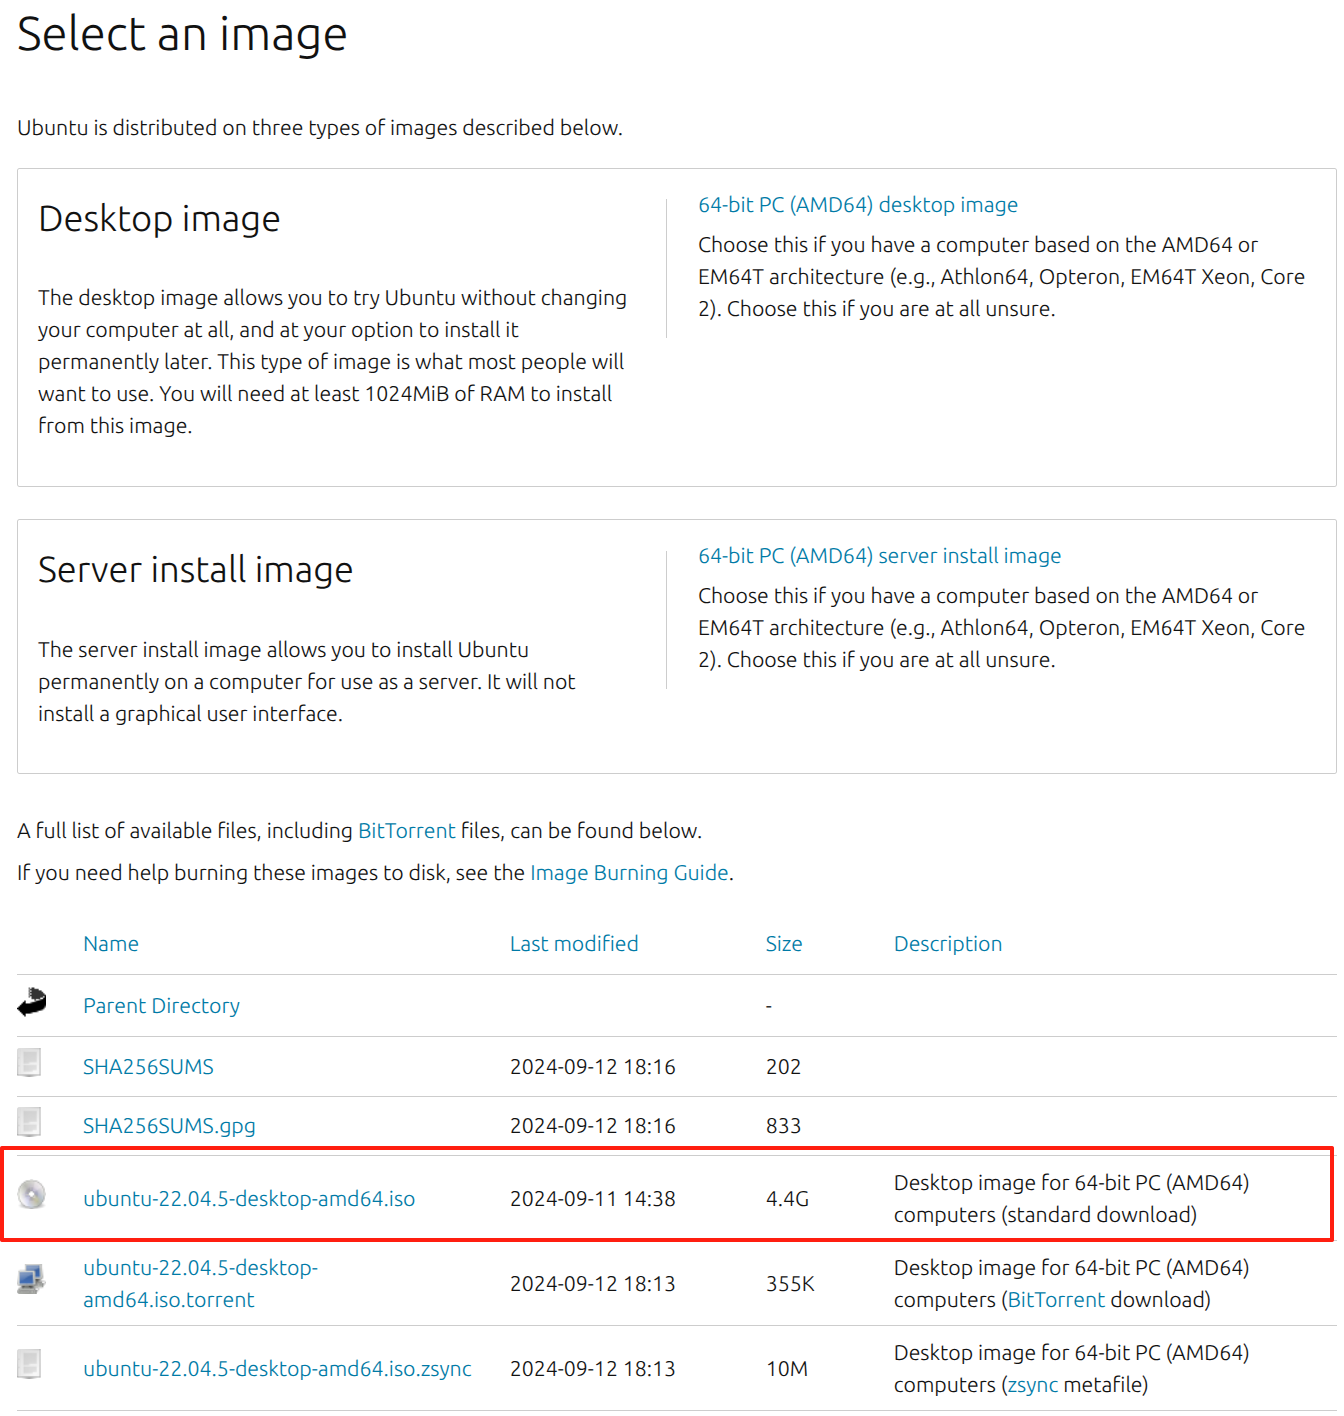
\includegraphics[width=0.9\textwidth]{figs/implementation/download_ubuntu_desktop.png}
%             \caption{下载Ubuntu 22.04 LTS的ISO镜像文件}
%             \label{fig:download_ubuntu_desktop}
%         \end{figure}
%     \item 如图所示，参照教程\href{https://ubuntu.com/tutorials/install-ubuntu-desktop#1-overview}{Install Ubuntu Desktop}完成OS的安装。
%         \begin{figure}[htbp]
%             \centering
%             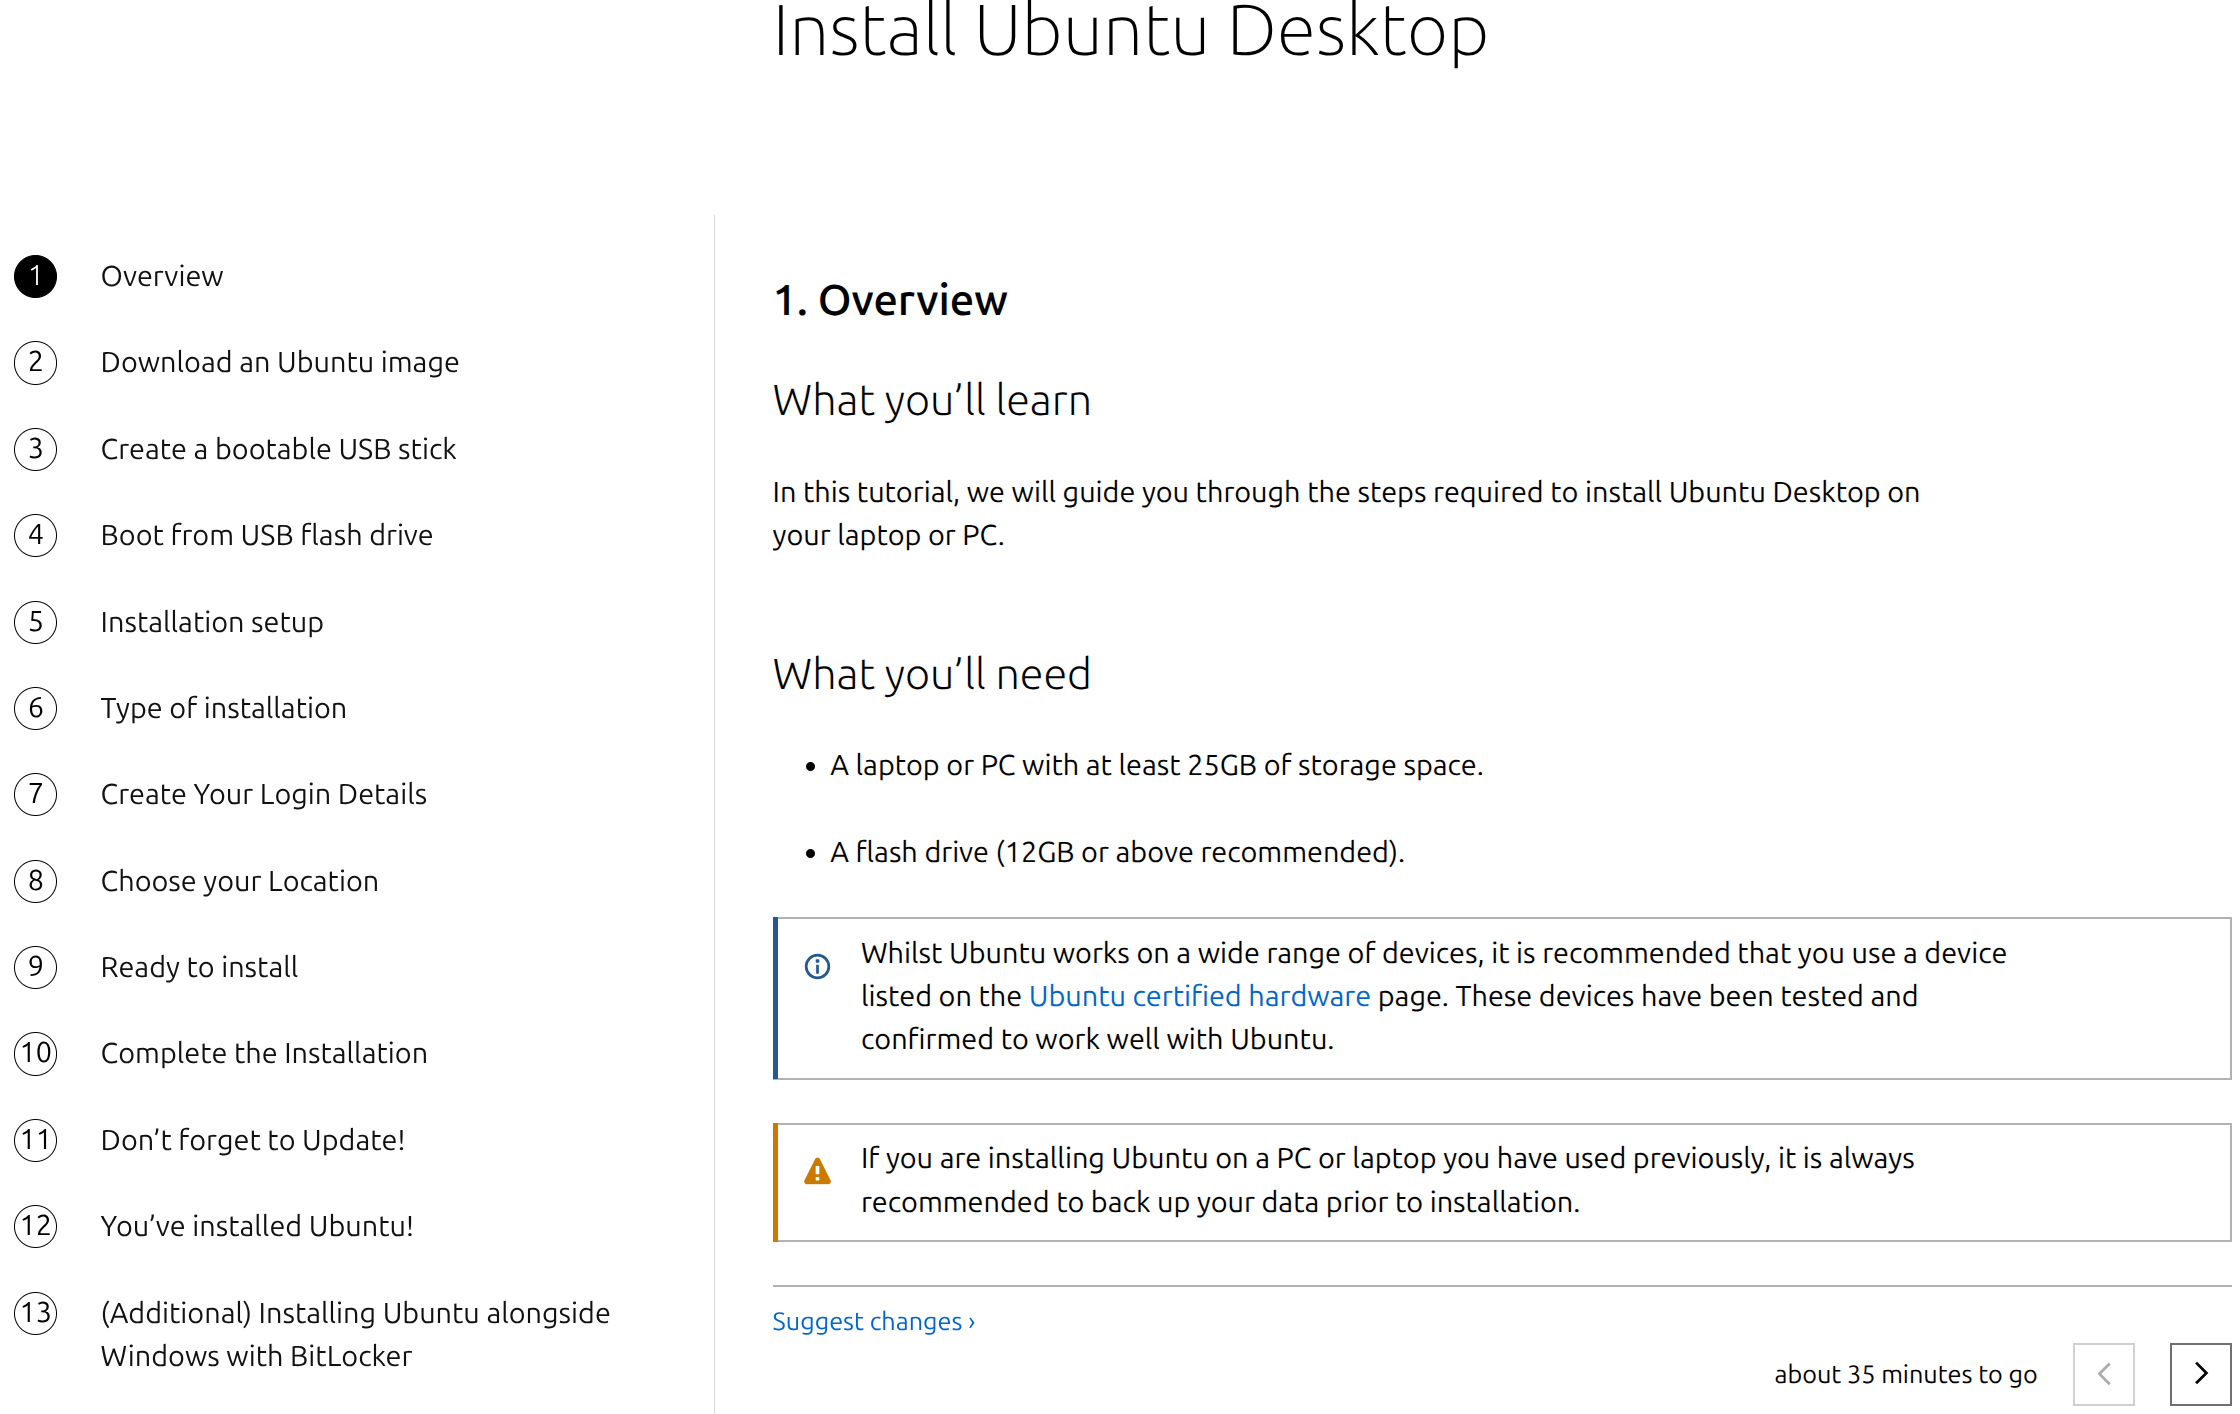
\includegraphics[width=0.9\textwidth]{figs/implementation/install_ubuntu_desktop.png}
%             \caption{安装Ubuntu 22.04 LTS}
%             \label{fig:install_ubuntu_desktop}
%         \end{figure}
% \end{enumerate}

% \subsubsection{安装ROS 2\label{subsubsec:ros_setup}}
% 本工程使用的ROS 2版本为Humble Hawksbill。按照教程\href{https://docs.ros.org/en/humble/Installation/Ubuntu-Install-Debs.html}{Ubuntu (deb packages)}逐步进行安装，执行完如图~\ref{fig:try_some_examples}所示的步骤即可。
% \begin{figure}[htbp]
%     \centering
%     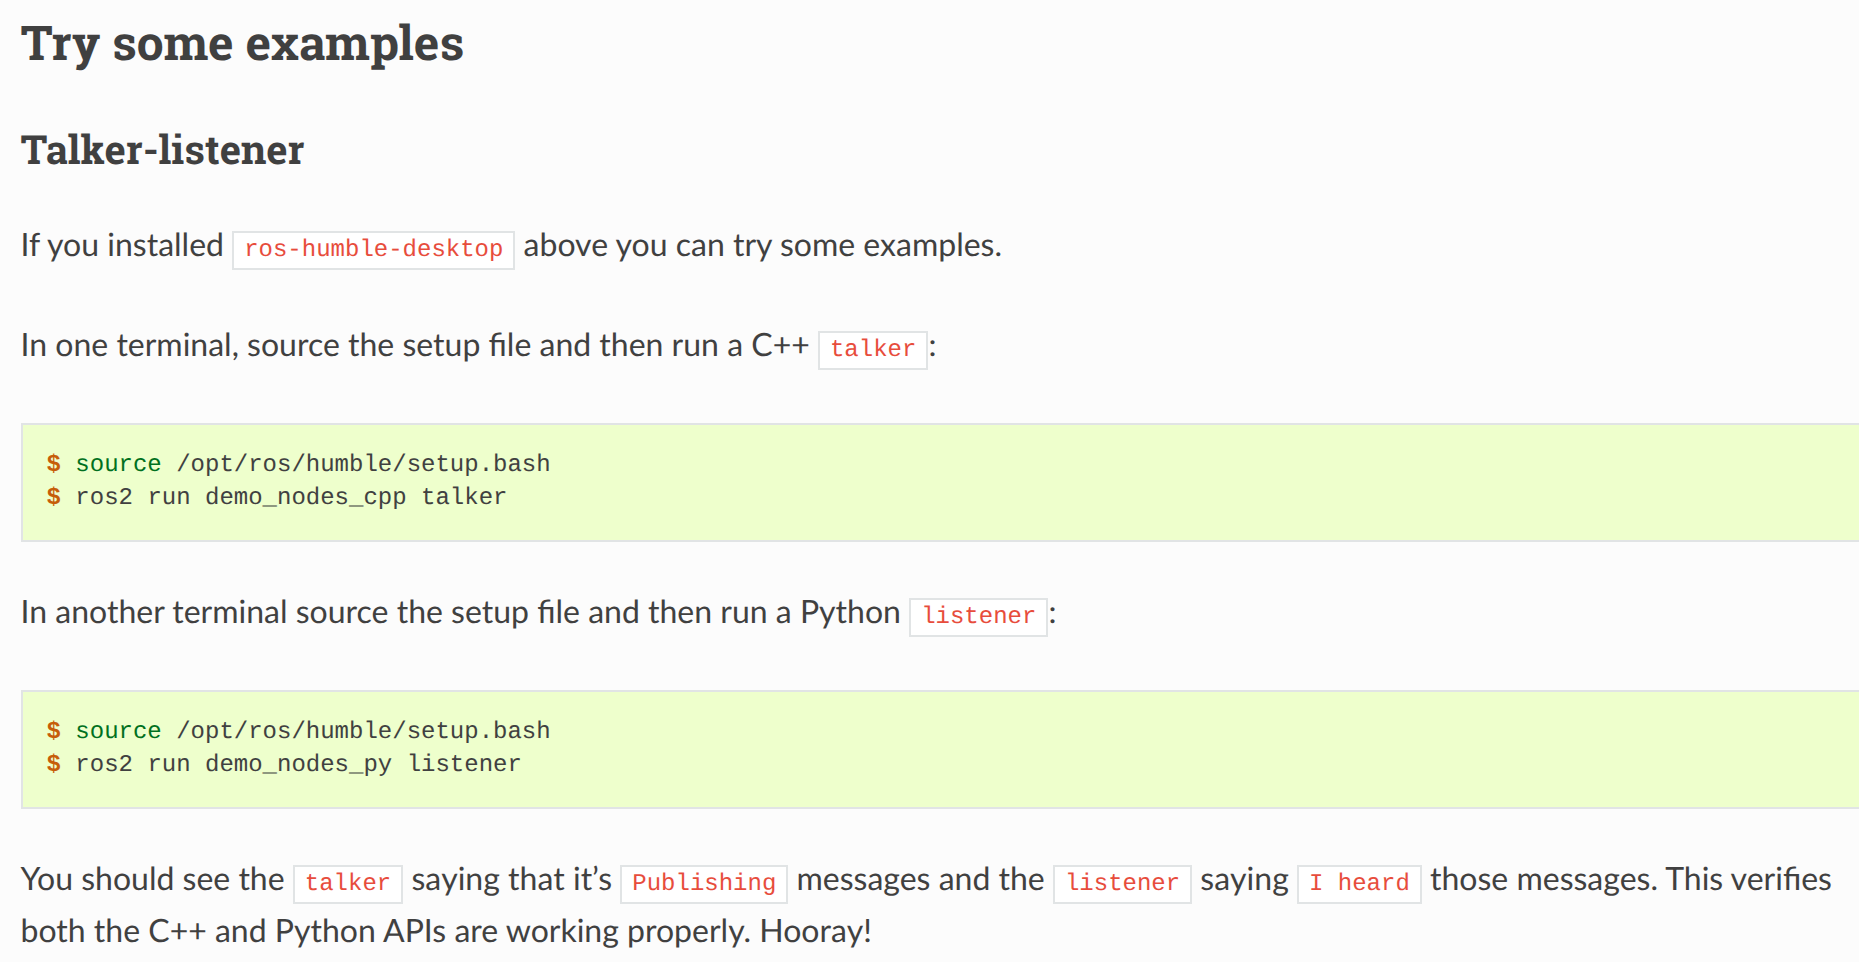
\includegraphics[width=0.9\textwidth]{figs/implementation/try_some_examples.png}
%     \caption{安装ROS 2 Humble Hawksbill}
%     \label{fig:try_some_examples}
% \end{figure}

% \subsubsection{安装功能包\label{subsubsec:packages_setup}}
% 在PC机上，本工程使用的功能包主要是Turtlebot3的、rtabmap的、navigation2的。
% [On PC] 相关安装命令如下：
% $ source /opt/ros/humble/setup.bash
% $ mkdir -p ~/ros2_ws/src
% $ cd ~/ros2_ws/src/
% $ git clone -b humble https://github.com/ROBOTIS-GIT/DynamixelSDK.git
% $ git clone -b humble https://github.com/ROBOTIS-GIT/turtlebot3_msgs.git
% $ git clone -b humble https://github.com/ROBOTIS-GIT/turtlebot3.git
% $ git clone https://github.com/introlab/rtabmap.git
% $ git clone -b ros2 https://github.com/introlab/rtabmap_ros.git
% $ git clone -b humble https://github.com/ros-navigation/navigation2.git
% $ git clone -b humble https://github.com/Jian-UOA/CS5917.git
% $ sudo apt install python3-colcon-common-extensions
% $ cd ~/ros2_ws
% $ colcon build --symlink-install

% \subsubsection{安装开发环境\label{subsubsec:dev_env_setup}}
% 本工程使用的开发环境为Visual Studio Code。安装步骤如下：
% \begin{enumerate}
%     \item 点击https://code.visualstudio.com/Download该链接，下载相应版本的Visual Studio (本工程中选的是x64), 如图~\ref{fig:download_vscode}所示。
%         \begin{figure}[htbp]
%             \centering
%             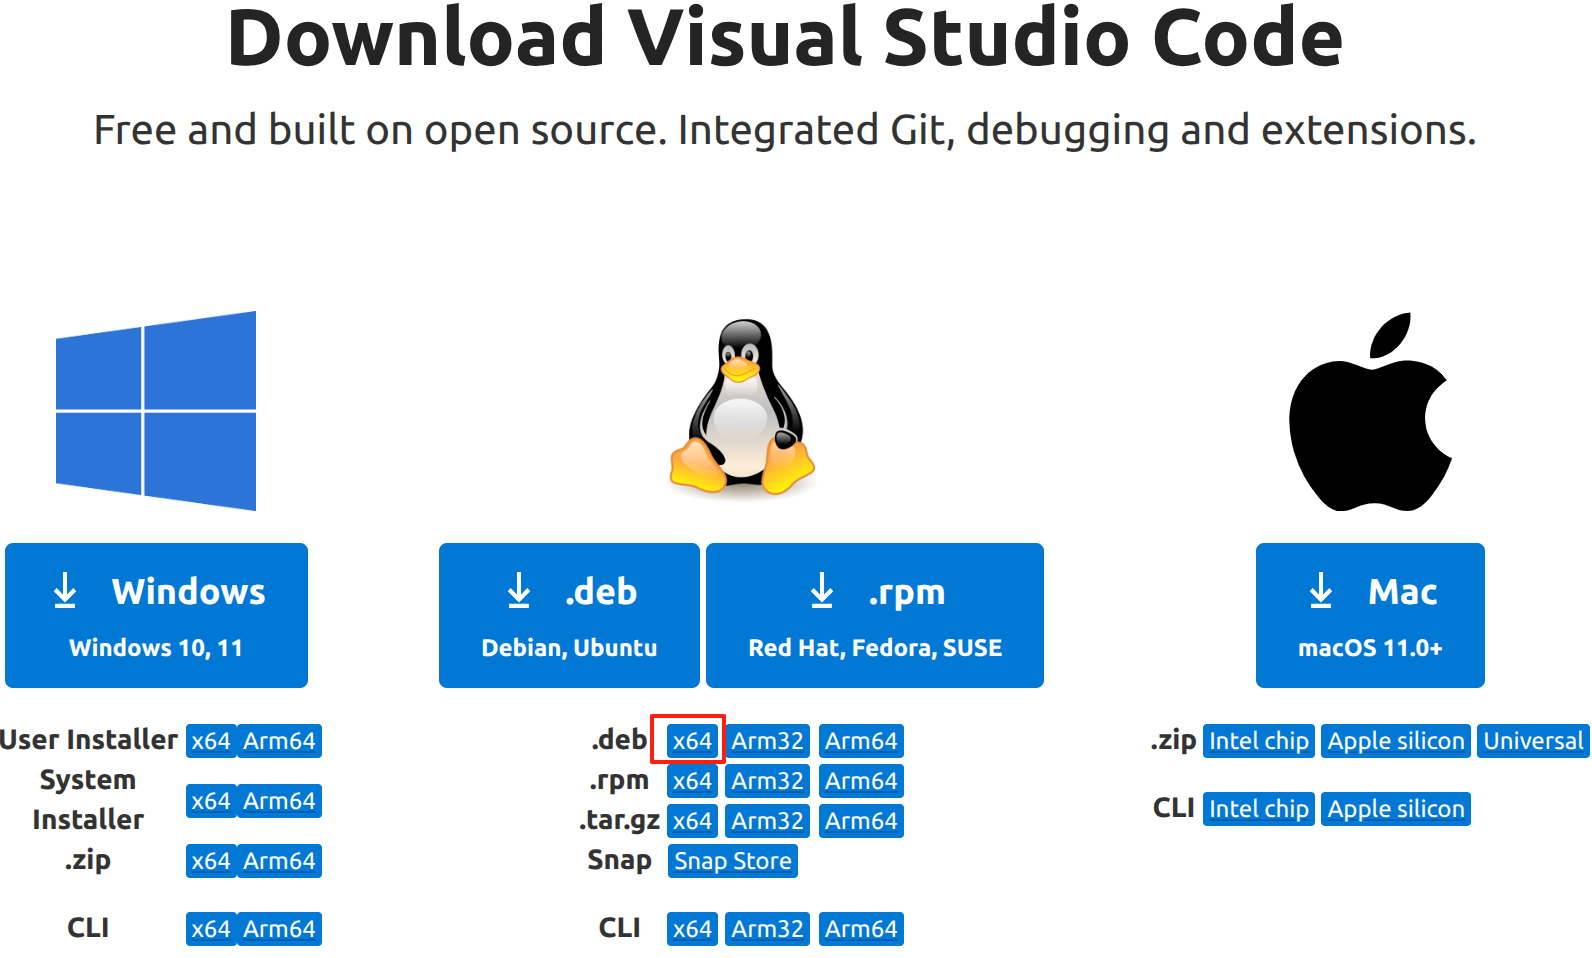
\includegraphics[width=0.9\textwidth]{figs/implementation/download_vscode.png}
%             \caption{下载Visual Studio Code}
%             \label{fig:download_vscode}
%         \end{figure}
%      \item 进入刚才下载文件的保存目录，找到下载的安装文件(\texttt{code_1.103.1-1755017277_amd64.deb})，按照教程\href{https://code.visualstudio.com/docs/setup/linux#_install-vs-code-on-linux}{Install VS Code on Linux}完成安装。如图~\ref{fig:install_vscode}所示。
%         \begin{figure}[htbp]
%             \centering
%             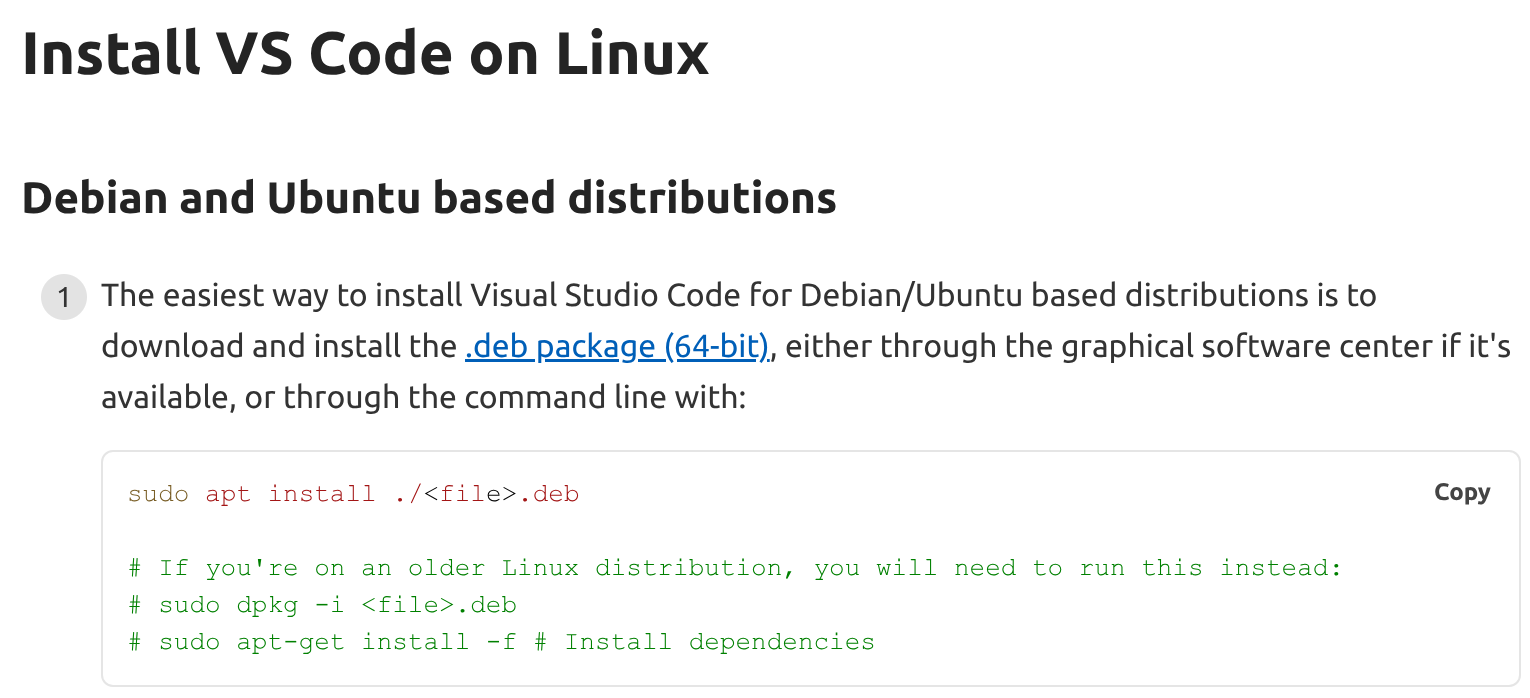
\includegraphics[width=0.9\textwidth]{figs/implementation/install_vscode.png}
%             \caption{安装Visual Studio Code}
%             \label{fig:install_vscode}
%         \end{figure}
%       \item 打开Visual Studio Code，按照教程\href{https://code.visualstudio.com/docs/getstarted/getting-started}{Tutorial: Get started with Visual Studio Code}中的示例，完成基本配置，打开目录\texttt{~/ros2_ws}中的工作空间，应该可以看到类似图~\ref{fig:open_ros2_ws}中的内容。
%         \begin{figure}[htbp]
%             \centering
%             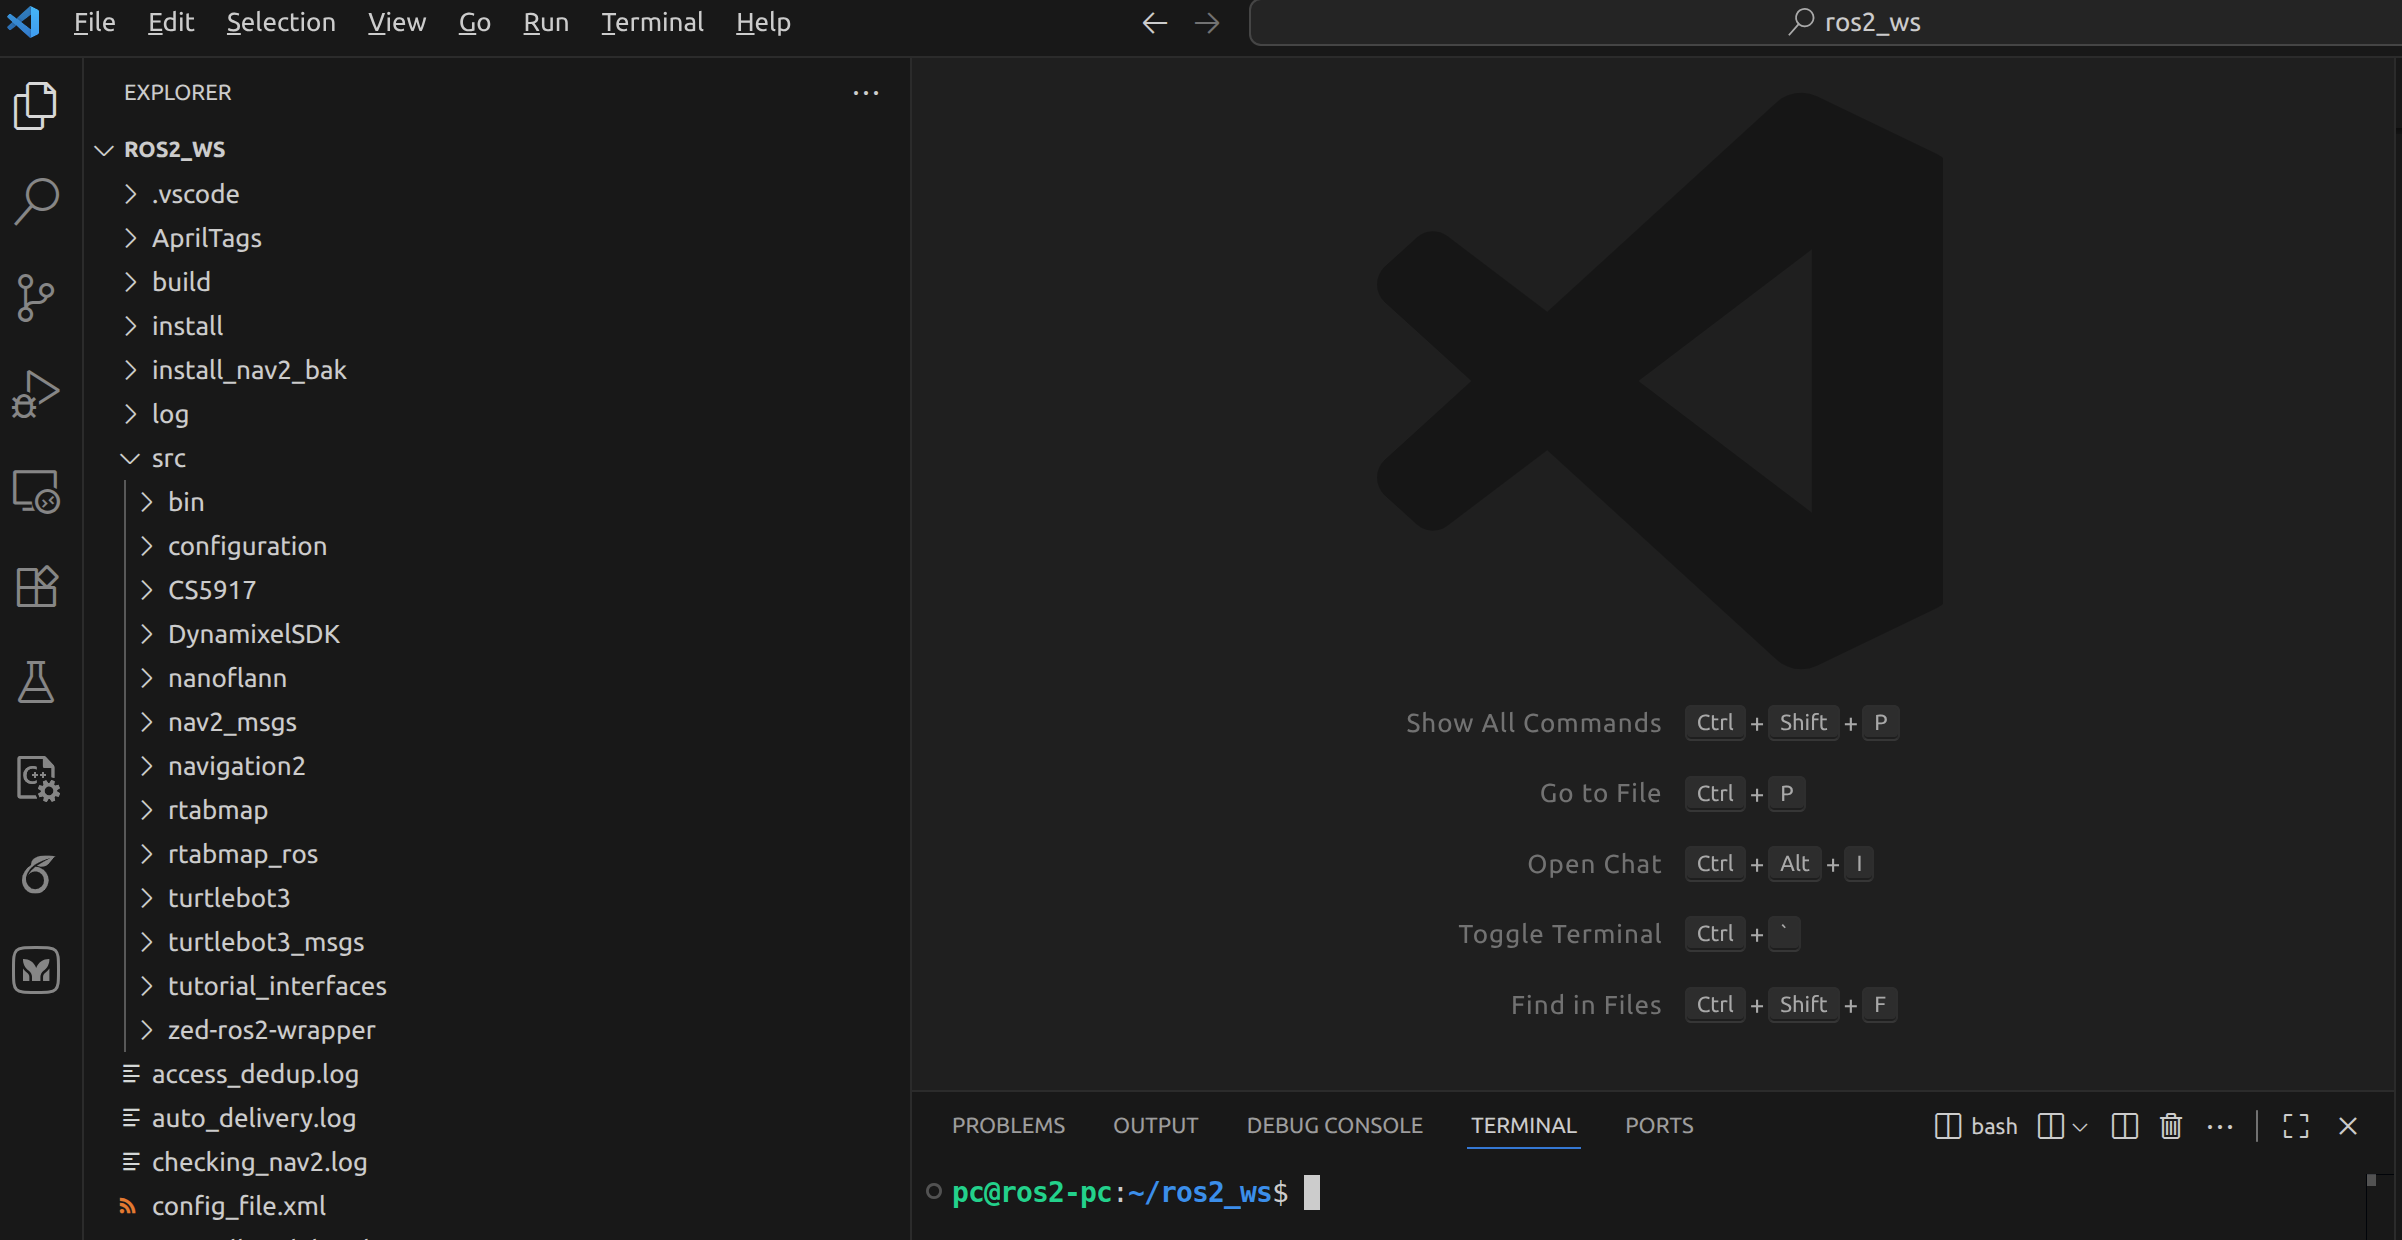
\includegraphics[width=0.9\textwidth]{figs/implementation/open_ros2_ws.png}
%             \caption{打开ROS 2工作空间}
%             \label{fig:open_ros2_ws}
%         \end{figure}
% \end{enumerate}

% \subsubsection{环境配置\label{subsubsec:env_setup}}
% [On PC] 相关配置命令如下：
% $ echo 'source ~/ros2_ws/install/setup.bash' >> ~/.bashrc
% $ echo 'source /opt/ros/humble/setup.bash' >> ~/.bashrc
% $ echo "export TURTLEBOT3_MODEL=waffle_pi" >> ~/.bashrc
% $ echo 'export ROS_DOMAIN_ID=30 #TURTLEBOT3' >> ~/.bashrc
% $ echo 'export RMW_IMPLEMENTATION=rmw_fastrtps_cpp' >> ~/.bashrc
% $ source ~/.bashrc

% \subsection{Turtlebot3\label{subsec:turtlebot3_setup}}
% 本工程使用的Turtlebot3为Waffle Pi版本，具体硬件配置参见\autoref{tab:turtlebot3_specs}。关于Turtlebot3上Sigle Board Computer (SBC) 和 OpenCR 的Setup, 请参见教程\href{https://emanual.robotis.com/docs/en/platform/turtlebot3/sbc_setup/#sbc-setup}{SBC Setup}和\href{https://emanual.robotis.com/docs/en/platform/turtlebot3/opencr_setup/#opencr-setup}{OpenCR Setup}。

% \subsection{Jetson Orin Nano\label{subsec:jetson_orin_nano_setup}}
% 本工程使用的Jetson Orin Nano为开发者套件版本，具体硬件配置参见\autoref{tab:jetson_orin_nano_specs}。在Jetson Orin Nano上，主要安装操作系统、ROS 2、双目相机ZED的SDK、ZED功能包、rtabmap功能包、本工程功能包uoa_robot_drone并进行相应环境配置，下面我们将详细介绍这些步骤。
% \subsubsection{安装操作系统\label{subsubsec:jetson_os_setup}}
    % \begin{enumerate}
    %     \item 按照教程\href{https://docs.nvidia.com/sdk-manager/download-run-sdkm/index.html}{Download and Run SDK Manager}免费注册账户后，通过SDK Manager安装6.2.1版本的Jet Pack。
    %     \item 图形界面进入Jetson Orin Nano的Ubuntu系统，连上无线网络。
    %     \item 为节省资源，SSH进入Jetson Orin Nano,输入命令：
    %     \begin{lstlisting}[language=bash]
    %         ssh username@ip_address
    %     \end{lstlisting}
    %     其中，\texttt{username}是Jetson Orin Nano的用户名，\texttt{ip_address}是Jetson Orin Nano的IP地址。
    %     \item 进入Jetson Orin Nano的Ubuntu系统后，输入命令：
    %     \begin{lstlisting}[language=bash]
    %         sudo systemctl set-default multi-user.target
    %         sudo systemctl reboot
    %     \end{lstlisting}
    %     \item 重新启动后，Jetson Orin Nano将进入命令行模式。
    % \end{enumerate}

    % \subsubsection{安装ROS 2\label{subsubsec:jetson_ros_setup}}
% 本工程使用的ROS 2版本为Humble Hawksbill。按照教程\href{https://docs.ros.org/en/humble/Installation/Ubuntu-Install-Debs.html}{Ubuntu (deb packages)}逐步进行安装，执行完如图~\ref{fig:try_some_examples}所示的步骤即可。

% \subsubsection{安装ZED SDK\label{subsubsec:zed_sdk_setup}}
% 本工程使用的ZED SDK为CUDA 12 ZED SDK for Ubuntu 22 5.0 版本。按照教程\href{https://www.stereolabs.com/docs/development/zed-sdk/linux}{Download and Install the ZED SDK}逐步进行安装，不建议在\texttt{silent mode}下安装。

% \subsubsection{安装功能包\label{subsubsec:jetson_packages_setup}}
% 在Jetson Orin Nano上，本工程使用的功能包主要是双目相机ZED 2的、rtabmap的 和本工程功能包\texttt{uoa_robot_drone}。
% [On Jetson Orin Nano] 相关安装命令如下：
% $ source ~/.bashrc
% $ mkdir -p ~/colcon_ws/src
% $ cd ~/colcon_ws
% $ git clone https://github.com/stereolabs/zed-ros2-wrapper.git src/zed-ros2-wrapper 
% $ git clone https://github.com/introlab/rtabmap.git src/rtabmap 
% $ git clone -b ros2 https://github.com/introlab/rtabmap_ros.git src/rtabmap_ros
% $ git clone -b humble https://github.com/Jian-UOA/CS5917.git src/CS5917
% $ sudo apt install python3-colcon-common-extensions
% $ colcon build --symlink-install

% \subsubsection{环境配置\label{subsubsec:jetson_env_setup}}
% [On Jetson Orin Nano] 相关配置命令如下：
% $ echo 'source ~/colcon_ws/install/setup.bash' >> ~/.bashrc
% $ echo 'source /opt/ros/humble/setup.bash' >> ~/.bashrc
% $ echo 'export ROS_DOMAIN_ID=30' >> ~/.bashrc
% $ echo 'export RMW_IMPLEMENTATION=rmw_fastrtps_cpp' >> ~/.bashrc
% $ source ~/.bashrc

% \subsubsection{验证安装\label{subsubsec:jetson_verify_setup}}
% 验证Jetson Orin Nano安装是否成功的步骤如下：
% \begin{enumerate}
%    \item 在PC上打开终端，使用SSH连接到Jetson Orin Nano后，输入命令：
%    \begin{lstlisting}[language=bash]
%        clear && cd ~/colcon_ws && ros2 launch zed_wrapper zed_camera.launch.py | tee zed.log
%    \end{lstlisting}
%    \item 如果zed相关安装成功，应该可以看到类似图~\ref{fig:zed_camera_launch}中的输出。


% English version:
\chapter{Implementation\label{chap:implementation}}
To enable readers to fully reproduce this engineering, this chapter will detail the implementation process, including hardware selection, environment setup, and software development.

\section{Hardware Selection}
% 中文版：
% 其实，做该工程的初衷是为了将一年来所学的AI知识尽可能多地通过工程化的方式转化到实际产品中去，以便让那些活跃在黑板上、实验室里的数学公式、算法模型能够真正地走进现实世界，帮助人们做些具体的实事。为节省成本起见，便看导师办公室里有哪些现成的硬件设备可以使用，就选择哪些设备来做该工程。经过与导师沟通，最终确定了以下硬件设备：

% English Version：
% Actually, the initial intention of this project is to transform the AI knowledge learned over the past year into practical products through engineering implementation, allowing mathematical formulas and algorithm models that are active on blackboards and in laboratories to truly enter the real world and help people accomplish specific tasks. To save costs, we looked at what existing hardware devices were available in the supervisor's office and chose those devices for this engineering. After discussions with the supervisor, the following hardware devices were finalized:
The hardware devices used in this engineering project are Turtlebot3 Waffle Pi, ZED 2 stereo camera, Jetson Orin Nano, INIU 65W 20000mAh power bank, DJI Tello EDU drone, and Lenovo laptop with 16GB RAM.

\subsection{Robot Platform -- Turtlebot3 Waffle Pi}
Turtlebot3 Waffle Pi is an open-source robot platform based on Raspberry Pi SBC, suitable for chassis. Its dimension graph is shown in Figure~\ref{fig:turtlebot3_dimensions}, and its components are shown in Figure~\ref{fig:turtlebot3_components}.
\begin{figure}[!h]
    \centering
    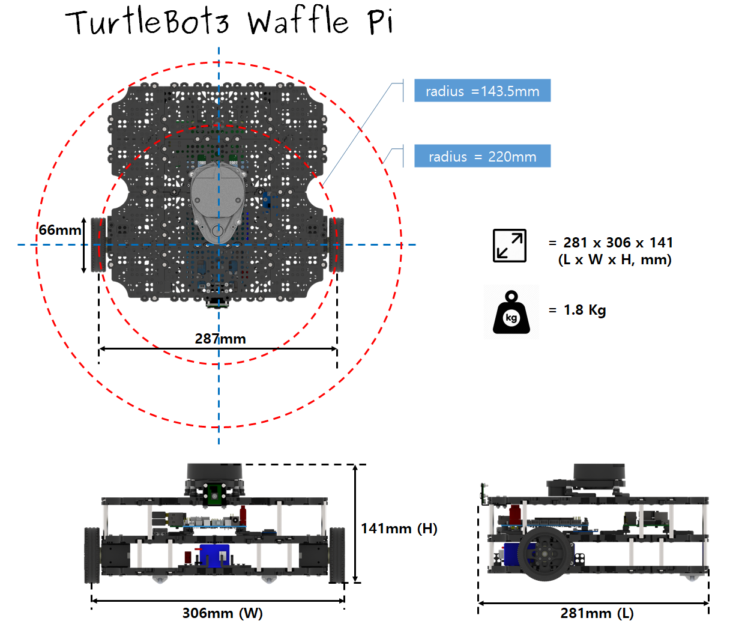
\includegraphics[height=0.60\textheight]{figs/tb3/turtlebot3_dimension3.png}
    \caption{Turtlebot3 Waffle Pi Dimensions and Mass}
    \label{fig:turtlebot3_dimensions}
\end{figure}
\begin{figure}[!h]
    \centering
    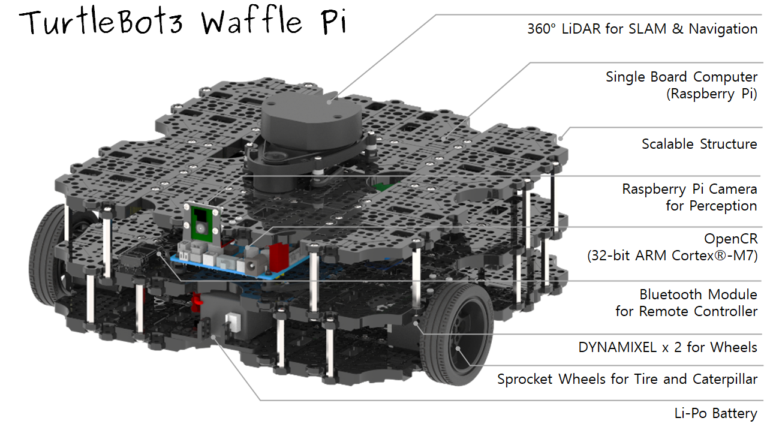
\includegraphics[width=0.90\textwidth]{figs/tb3/turtlebot3_waffle_pi_components.png}
    \caption{Turtlebot3 Waffle Pi Components (Note: The LiDAR sensor shown in this figure is not used in this project, as we employ pure vision-based SLAM)}
    \label{fig:turtlebot3_components}
\end{figure}
For more detailed specifications and component lists of Turtlebot3 Waffle Pi, please refer to Appendix~\ref{sec:turtlebot3_details}.

\subsection{Stereo Vision Camera -- ZED 2}
ZED 2 is a high-performance stereo vision camera, used for visual SLAM and environment perception. Its front view is shown in Figure~\ref{fig:zed2_camera}.
\begin{figure}[htbp]
    \centering
    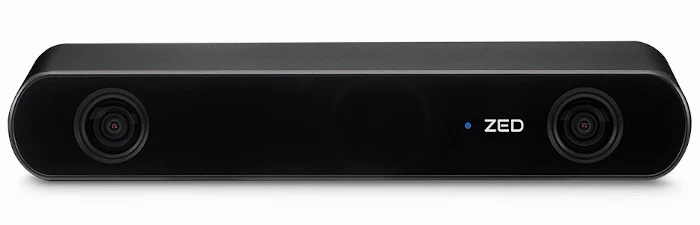
\includegraphics[width=0.9\textwidth]{figs/zed2/ZED-2-front.png}
    \caption{ZED 2 Stereo Vision Camera}
    \label{fig:zed2_camera}
\end{figure}
For more detailed specifications of ZED 2, please refer to Appendix~\ref{sec:zed2_details}.

\subsection{Edge Computing Unit -- Jetson Orin Nano}
Regarding the selection of the edge computing unit, NVIDIA has released various configurations of single\-board computers, including 4GB, 8GB, 16GB, 32GB, 64GB, and 128GB. Considering the actual requirements of this project, we chose the Jetson Orin Nano 8GB version. It is a lightweight embedded edge computing single\-board computer launched by NVIDIA, suitable for AI inference and edge computing tasks. Its layout diagram is shown in Figure~\ref{fig:jetson_orin_nano_layout}, and its components are listed in Table~\ref{tab:jetson_orin_nano_components}.

    \begin{figure}[h]
        \centering
        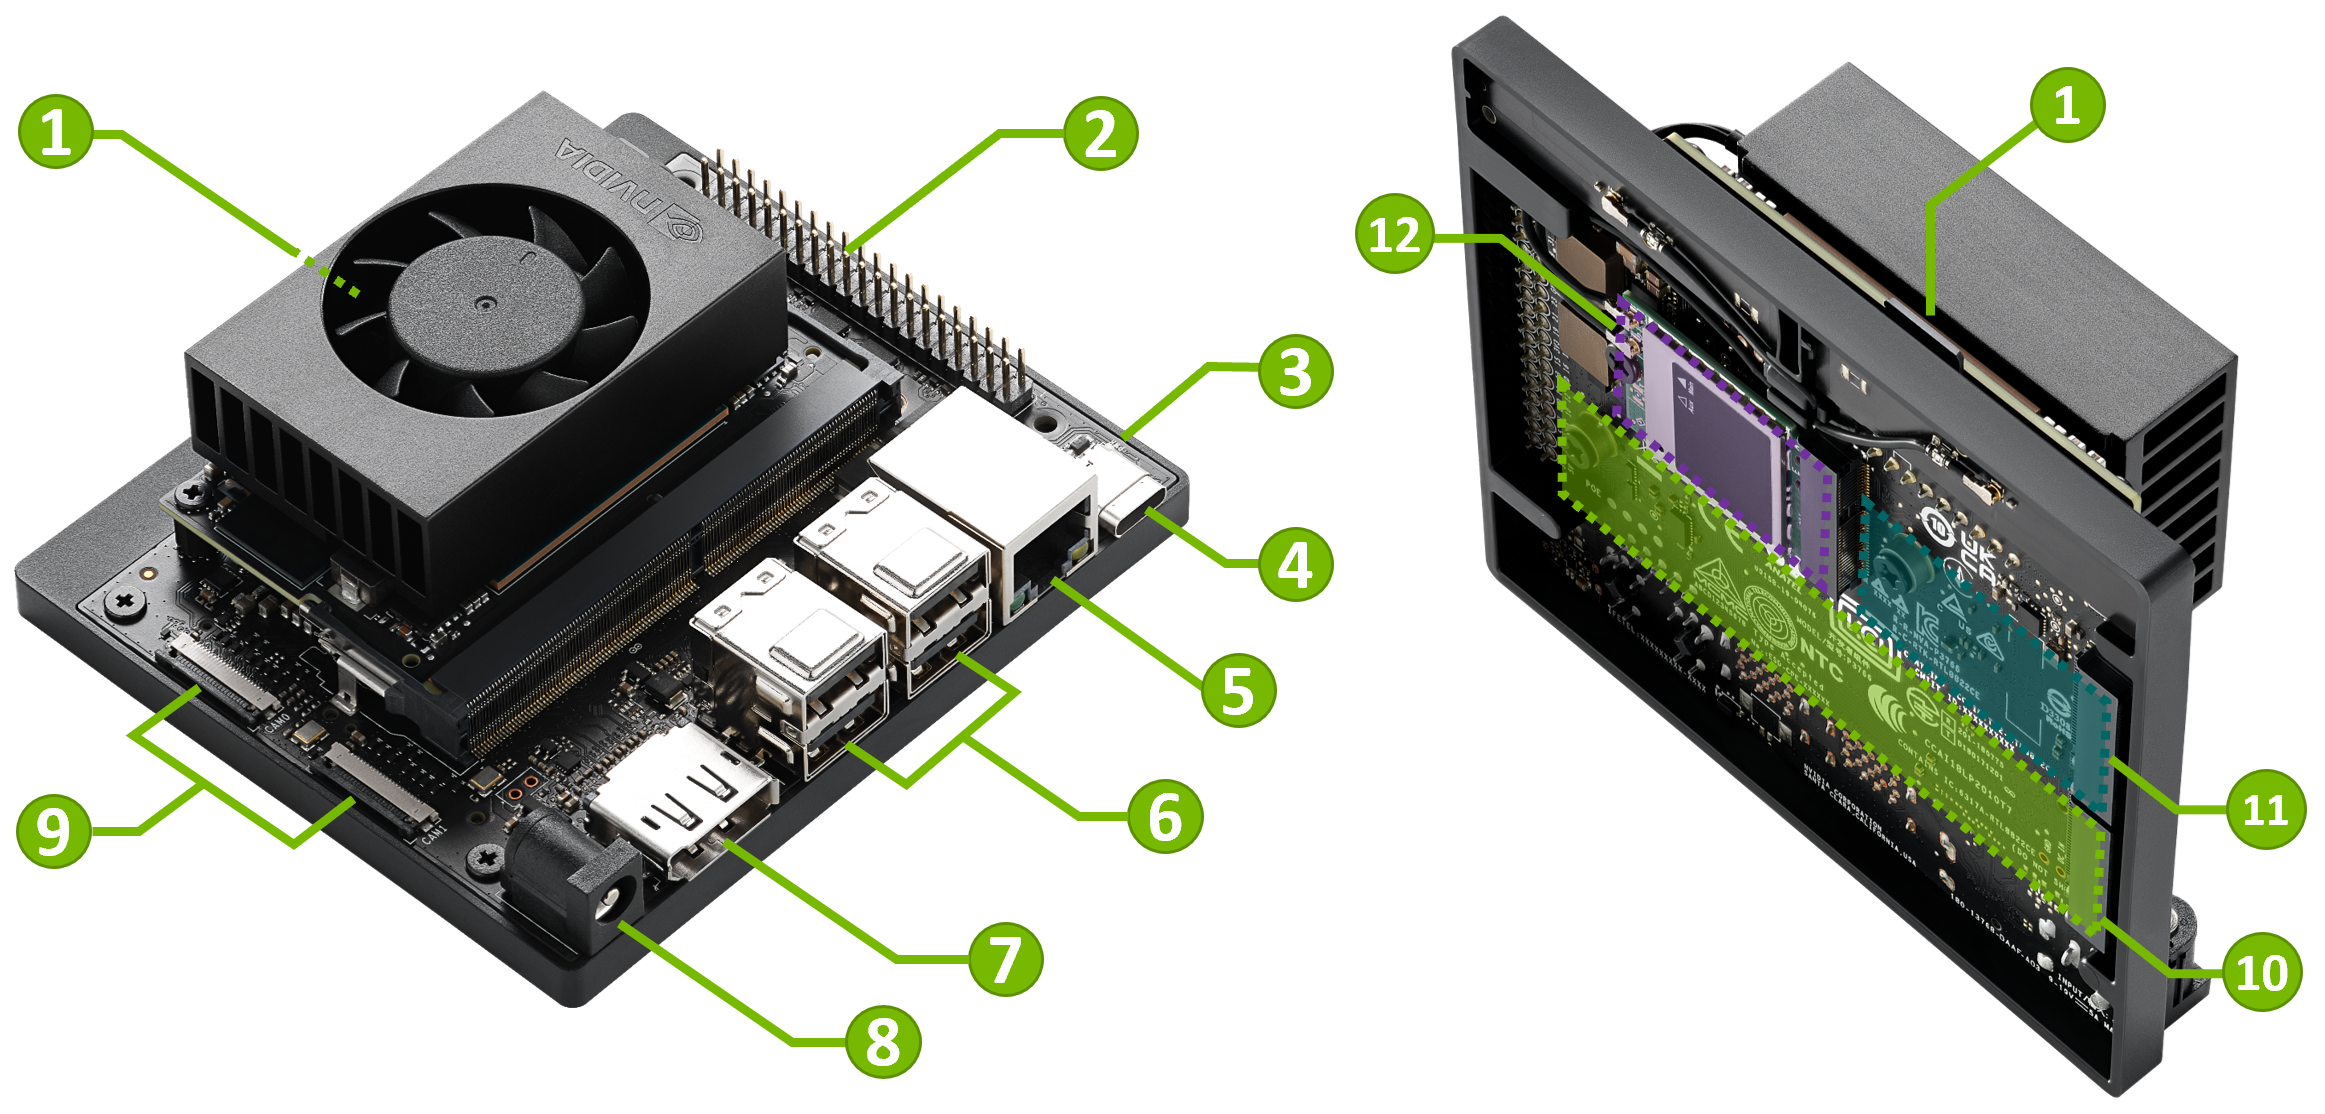
\includegraphics[width=0.9\textwidth]{figs/orin/jetson-nano-dev-kit_2view_numbered.png}
        \caption{Jetson Orin Nano Layout Diagram}
        \label{fig:jetson_orin_nano_layout}
    \end{figure}
    \begin{table}[h]
        \centering
        \caption{Jetson Orin Nano Components}
        \label{tab:jetson_orin_nano_components}
        \begin{tabular}{|c|l|p{6cm}|}
            \hline
            \textbf{Mark} & \textbf{Name} & \textbf{Note} \\
            \hline
            1 & microSD card slot & \\
            \hline
            2 & 40-pin Expansion Header & \\
            \hline
            3 & Power Indicator LED & \\
            \hline
            4 & USB-C port & For data only \\
            \hline
            5 & Gigabit Ethernet Port & \\
            \hline
            6 & USB 3.2 Type-A ports (x4) & 10Gbps \\
            \hline
            7 & DisplayPort Output Connector & \\
            \hline
            8 & DC Power Jack & 5.5mm x 2.5mm \\
            \hline
            9 & MIPI CSI Camera Connectors (x2) & 22pin, 0.5mm pitch \\
            \hline
            10 & M.2 Slot (Key-M, Type 2280) & PCIe 3.0 x4 \\
            \hline
            11 & M.2 Slot (Key-M, Type 2230) & PCIe 3.0 x2 \\
            \hline
            12 & M.2 Slot (Key-E, Type 2230) & (populated) \\
            \hline
        \end{tabular}
    \end{table}

\subsection{Power Supply -- INIU Power Bank}
 When selecting a power bank to supply power to the Jetson Orin Nano, we considered stability and chose a product with a voltage of up to 20V and a maximum output power of at least 65W. The INIU Power Bank was selected for this purpose. It has a capacity of 20000mAh and can output 65W at 20V, which is sufficient to power the Jetson Orin Nano. Its appearance is shown in Figure~\ref{fig:iniu_power_bank}.
\begin{figure}[htbp]
    \centering
    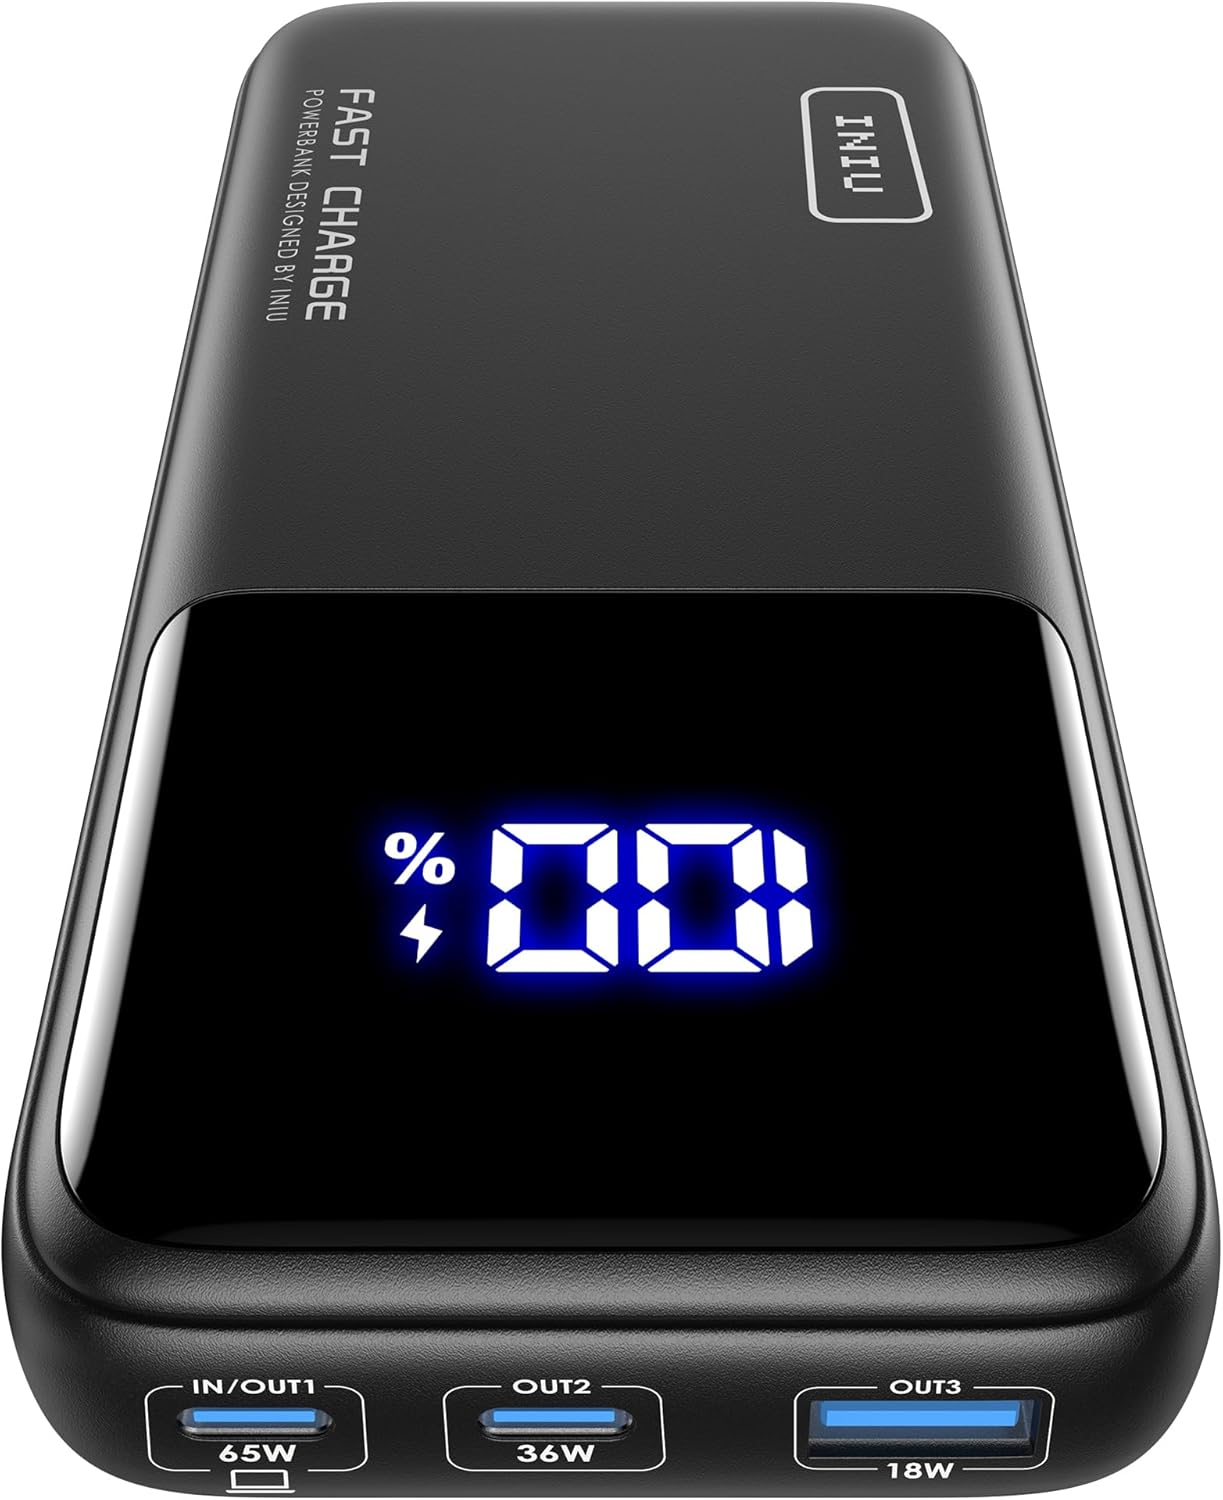
\includegraphics[width=0.5\textwidth]{figs/iniu/iniu_power_bank.jpg}
    \caption{INIU 65W 20000mAh Power Bank}
    \label{fig:iniu_power_bank}
\end{figure}
For more detailed specifications of INIU Power Bank, please refer to Appendix~\ref{sec:iniu_details}.

\subsection{Drone -- DJI Tello EDU}
To validate the feasibility of multi\-agent collaboration, this engineering selected the DJI Tello EDU drone. This drone is compact and lightweight, suitable for indoor flight and programming education. Its appearance is shown in Figure~\ref{fig:tello_edu_drone}. 

\begin{figure}[htbp]
    \centering
    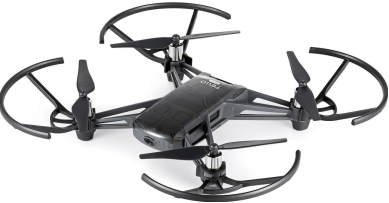
\includegraphics[width=0.5\textwidth]{figs/tello/tello_edu_drone.png}
    \caption{DJI Tello EDU Drone}
    \label{fig:tello_edu_drone}
\end{figure}
For more detailed specifications of DJI Tello EDU, please refer to Appendix~\ref{sec:tello_details}.

\subsection{Monitoring System -- Lenovo Laptop Yoga 14s 2021}
The monitoring system for this project uses a Lenovo laptop with 16GB of RAM, suitable for data processing and visualization tasks. 
For more detailed specifications of Lenovo Laptop Yoga 14s 2021, please refer to Appendix~\ref{sec:lenovo_details}.

\section{Environment Setup}
In this section, we will introduce how to set up the environment required for this engineering project, including the PC, Turtlebot3, and Jetson Orin Nano.

\subsection{PC Setup\label{subsec:pc_setup}}
This engineering project uses a standard laptop as the PC. The specific hardware configuration is shown in Table~\ref{tab:lenovo_laptop_specs}. On the PC, we mainly install the operating system, ROS 2, rtabmap package, the engineering package \texttt{uoa\_robot\_drone} and the development environment VS Code, and perform the corresponding environment configuration. Below, we will detail these steps.

\subsubsection{\textbf{Installing the Operating System}\label{subsubsec:os_setup}}
This engineering project uses Ubuntu 22.04 LTS as the operating system. *Note: To avoid issues, it is essential to install the OS using the \textbf{physical machine direct installation} method, not in a virtual machine (as Ubuntu on a virtual machine often fails during the Jetson Orin Nano flashing process). The installation steps are as follows:
\begin{enumerate}
    \item Click on the link https://releases.ubuntu.com/22.04/ to download the ISO image file of Ubuntu 22.04 LTS, as shown in Figure~\ref{fig:download_ubuntu_desktop}.
        \begin{figure}[!h]
            \centering
            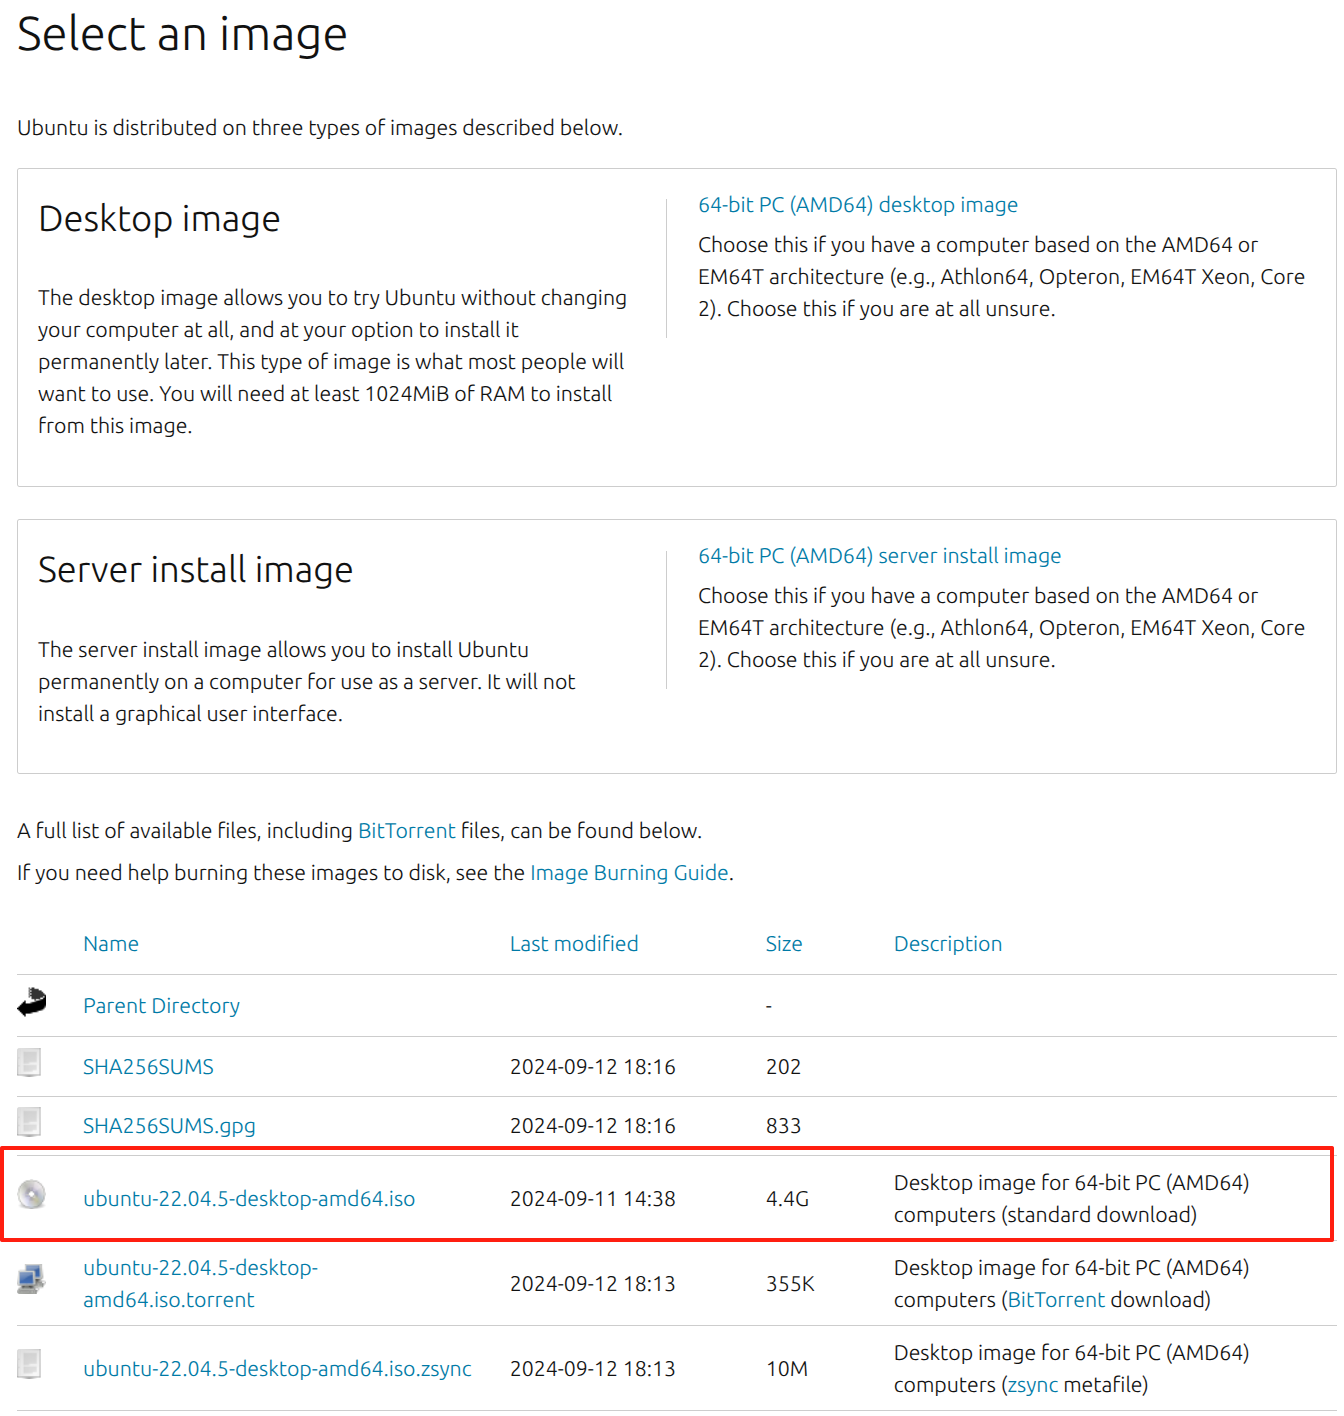
\includegraphics[width=0.9\textwidth]{figs/implementation/download_ubuntu_desktop.png}
            \caption{Downloading the ISO Image File of Ubuntu 22.04 LTS}
            \label{fig:download_ubuntu_desktop}
        \end{figure}
    \item Follow the tutorial \href{https://ubuntu.com/tutorials/install-ubuntu-desktop#1-overview}{Install Ubuntu Desktop} to complete the OS installation, as shown in Figure~\ref{fig:install_ubuntu_desktop}.
        \begin{figure}[!h]
            \centering
            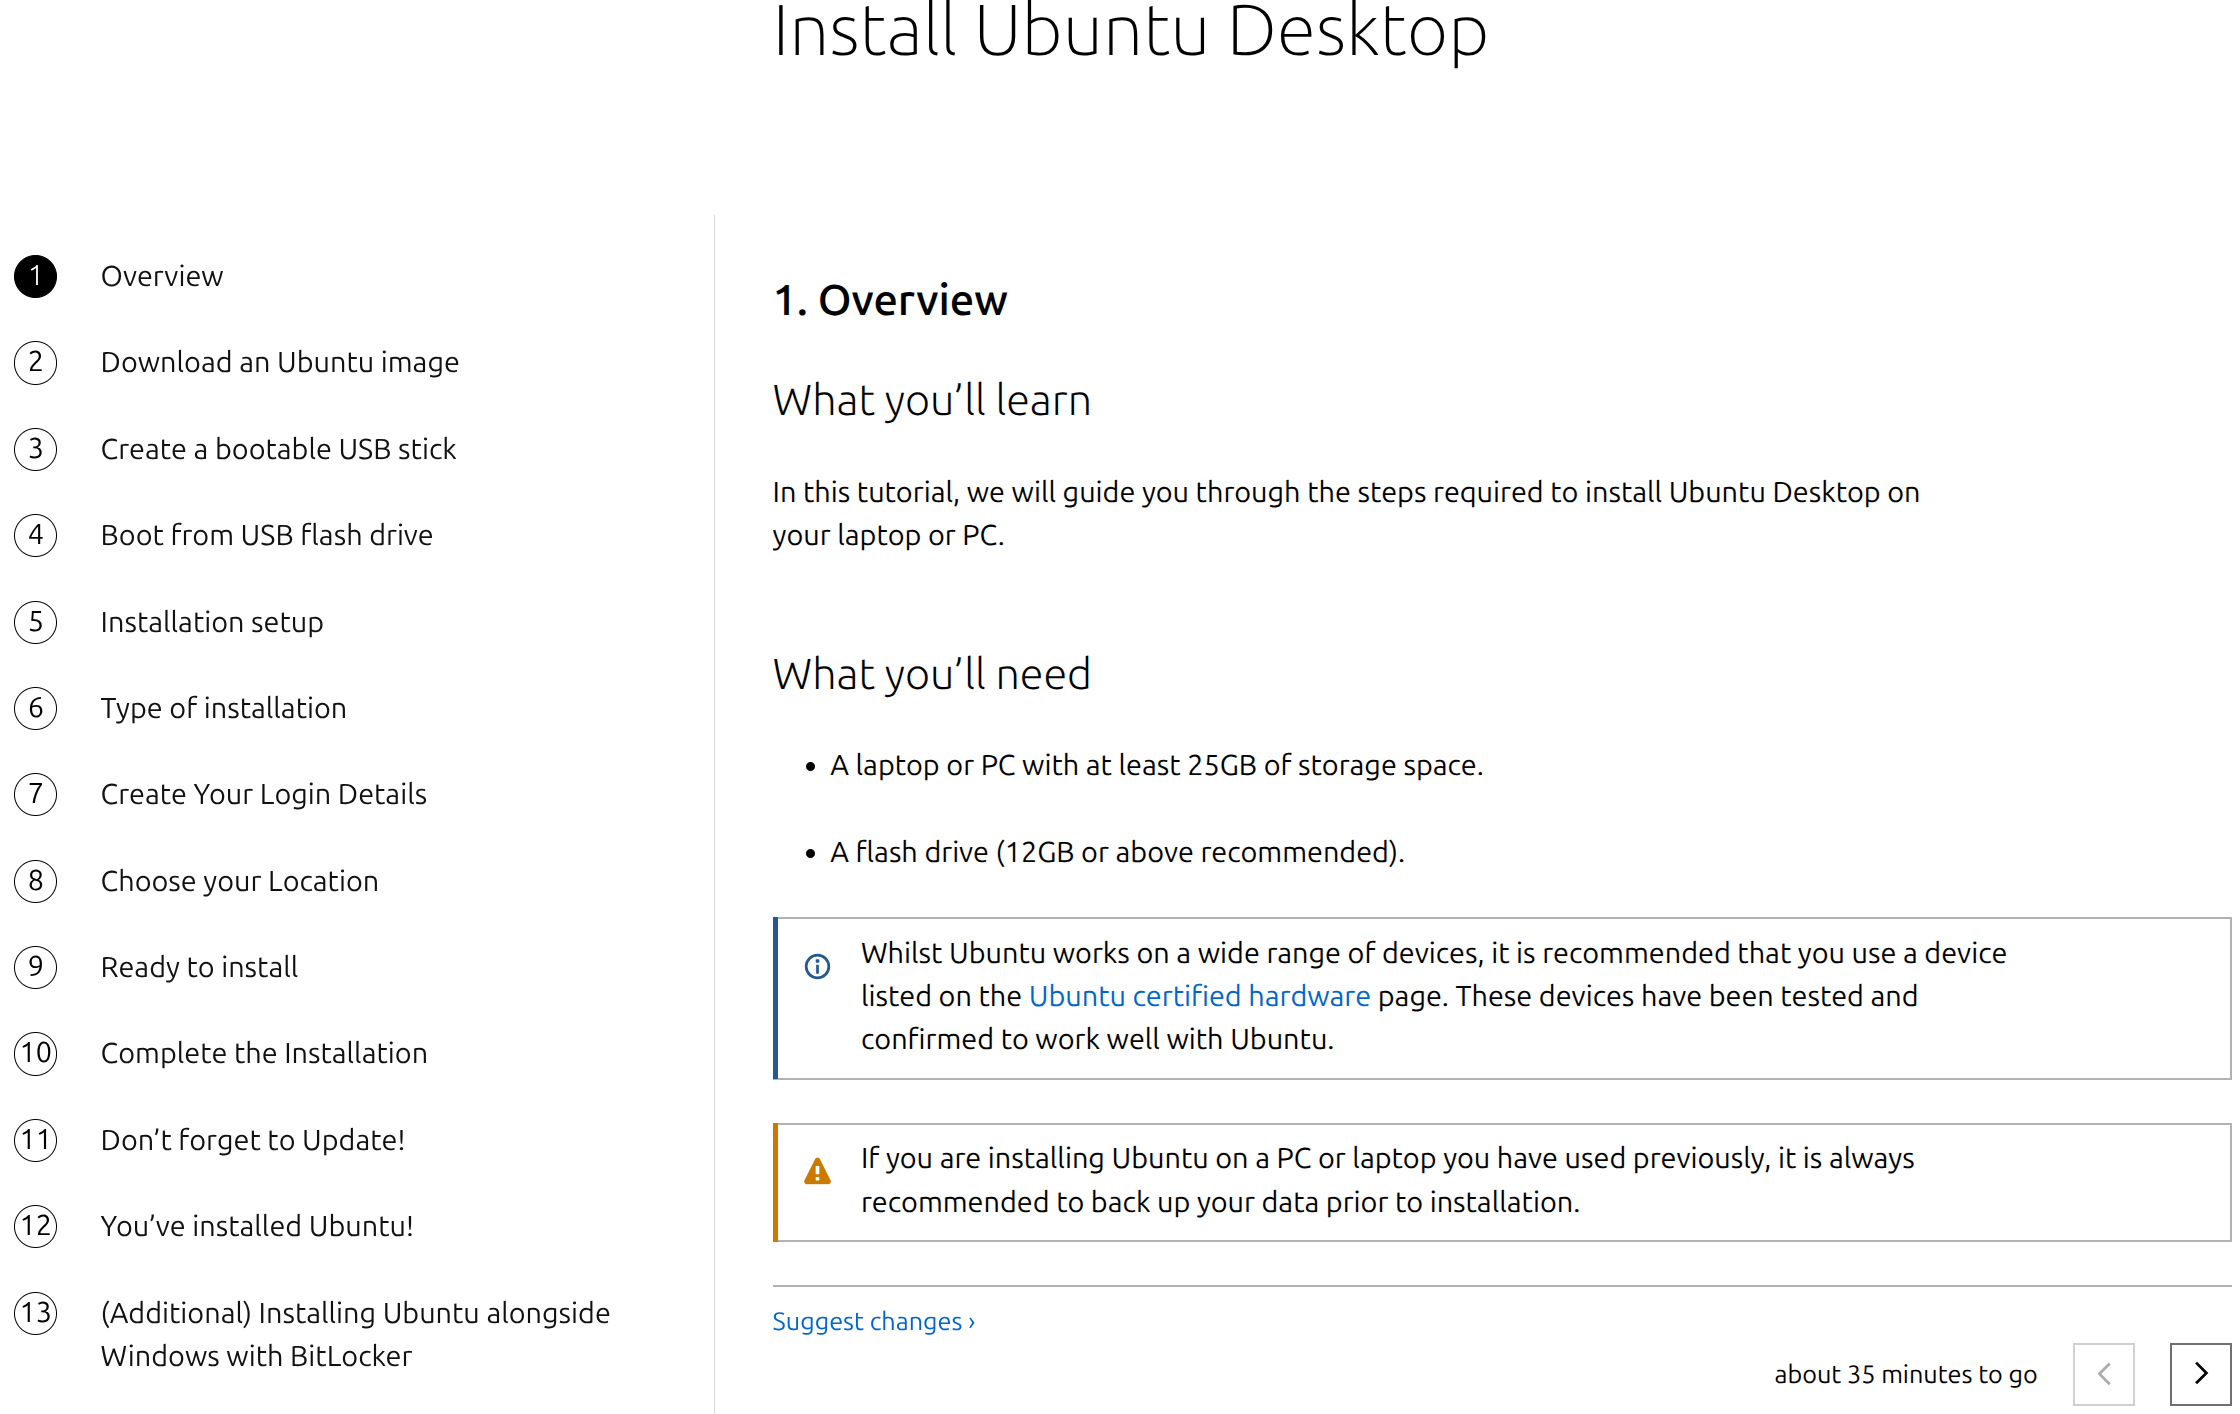
\includegraphics[width=0.9\textwidth]{figs/implementation/install_ubuntu_desktop.png}
            \caption{Installing Ubuntu 22.04 LTS}
            \label{fig:install_ubuntu_desktop}
        \end{figure}
\end{enumerate}

\subsubsection{\textbf{Installing ROS 2}\label{subsubsec:ros_setup}}
This engineering project uses ROS 2 Humble Hawksbill as the version. Follow the tutorial \href{https://docs.ros.org/en/humble/Installation/Ubuntu-Install-Debs.html}{Ubuntu (deb packages)} to install step by step, and execute the steps shown in Figure~\ref{fig:try_some_examples}.
\begin{figure}[!h]
    \centering
    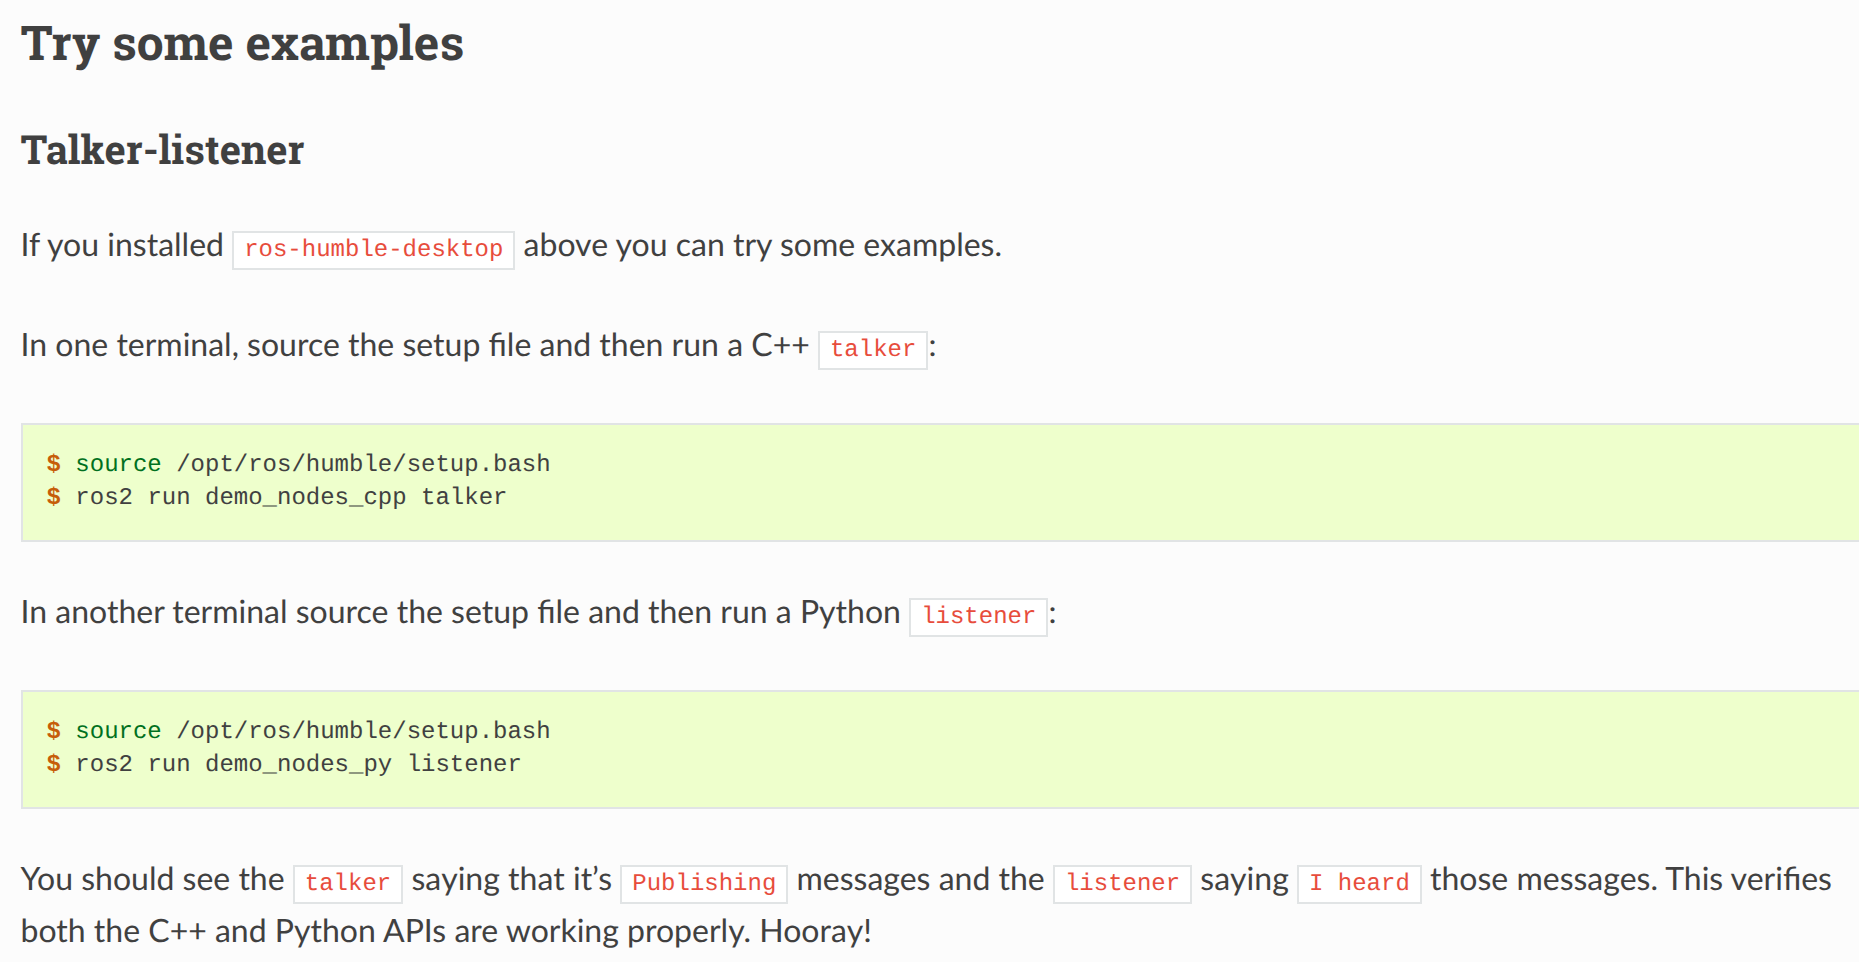
\includegraphics[width=0.9\textwidth]{figs/implementation/try_some_examples.png}
    \caption{Installing ROS 2 Humble Hawksbill}
    \label{fig:try_some_examples}
\end{figure}   

\subsubsection{\textbf{Installing Packages}\label{subsubsec:packages_setup}}
On the PC, the main packages used in this engineering project are Turtlebot3, rtabmap, and navigation2.
[On PC] The relevant installation commands are as follows:
\begin{lstlisting}[language=bash]
$ source /opt/ros/humble/setup.bash
$ mkdir -p ~/ros2_ws/src
$ cd ~/ros2_ws/src/
$ git clone -b humble https://github.com/ROBOTIS-GIT/DynamixelSDK.git
$ git clone -b humble https://github.com/ROBOTIS-GIT/turtlebot3_msgs.git
$ git clone -b humble https://github.com/ROBOTIS-GIT/turtlebot3.git
$ git clone https://github.com/introlab/rtabmap.git
$ git clone -b ros2 https://github.com/introlab/rtabmap_ros.git
$ git clone -b humble https://github.com/ros-navigation/navigation2.git
$ git clone -b humble https://github.com/Jian-UOA/CS5917.git
$ sudo apt install python3-colcon-common-extensions
$ cd ~/ros2_ws
$ colcon build --symlink-install
\end{lstlisting}

\subsubsection{\textbf{Installing the Development Environment}\label{subsubsec:dev_env_setup}}
This engineering project uses Visual Studio Code as the development environment. The installation steps are as follows:
\begin{enumerate}
    \item Click on the link https://code.visualstudio.com/Download to download the appropriate version of Visual Studio Code (in this engineering project, the x64 version is selected), as shown in Figure~\ref{fig:download_vscode}.
        \begin{figure}[!h]
            \centering
            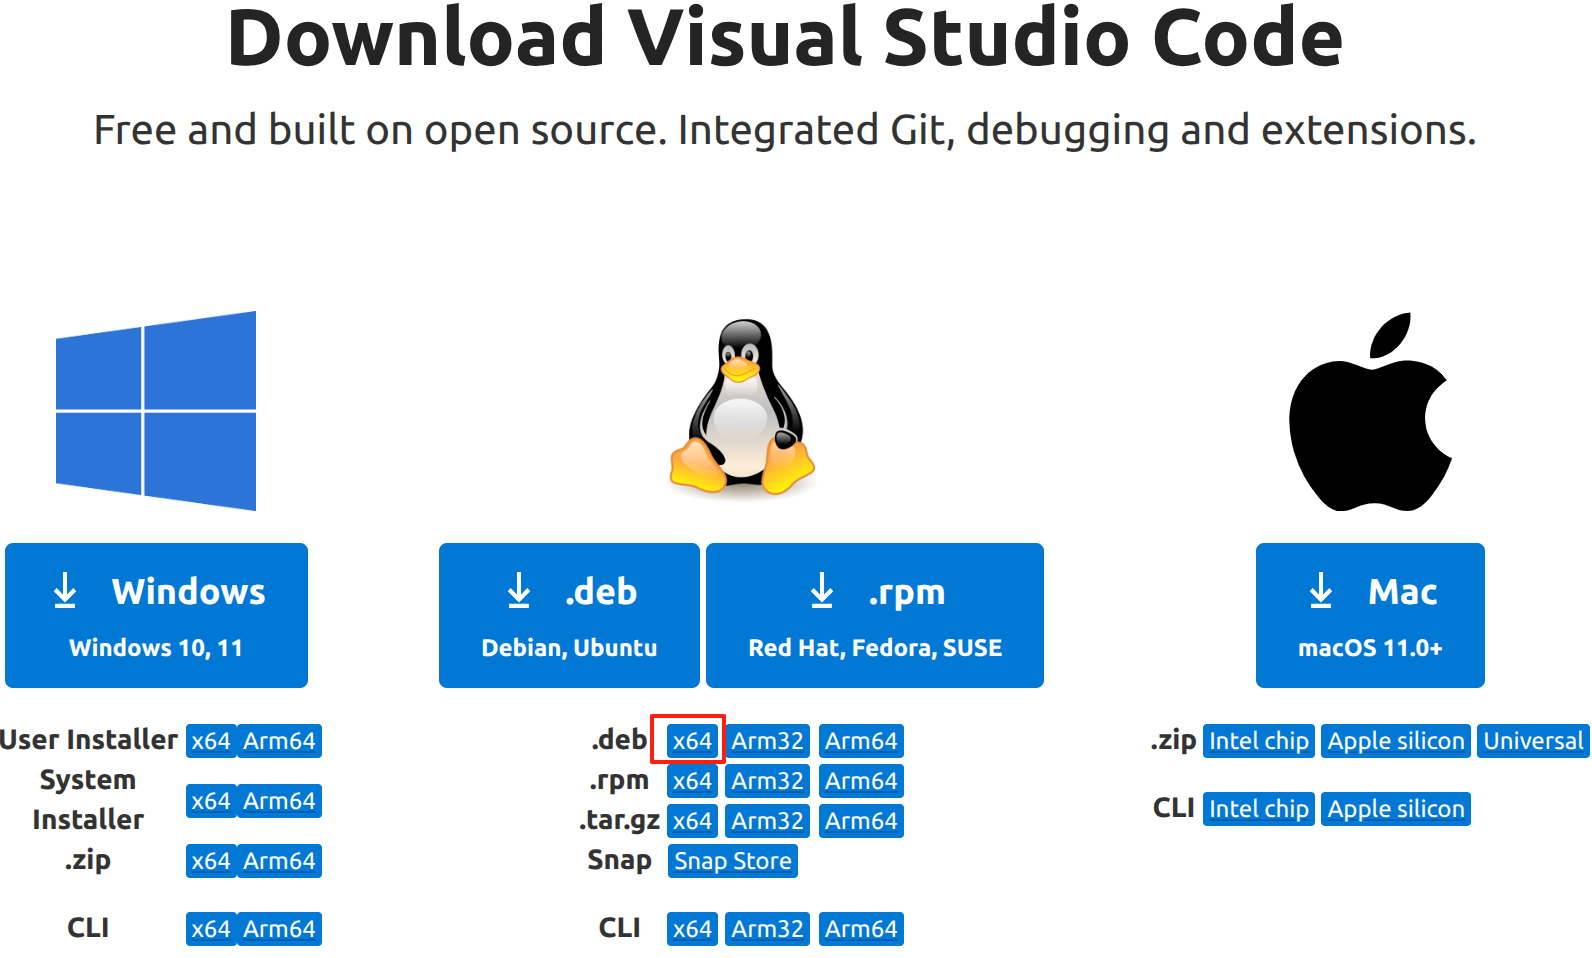
\includegraphics[width=0.9\textwidth]{figs/implementation/download_vscode.png}
            \caption{Downloading Visual Studio Code}
            \label{fig:download_vscode}
        \end{figure}
    \item Go to the directory where the downloaded file is saved, find the downloaded installation file (\texttt{code\_1.103.1-1755017277\_amd64.deb}), and follow the tutorial \href{https://code.visualstudio.com/docs/setup/linux#_install-vs-code-on-linux}{Install VS Code on Linux} to complete the installation, as shown in Figure~\ref{fig:install_vscode}.
        \begin{figure}[!h]
            \centering
            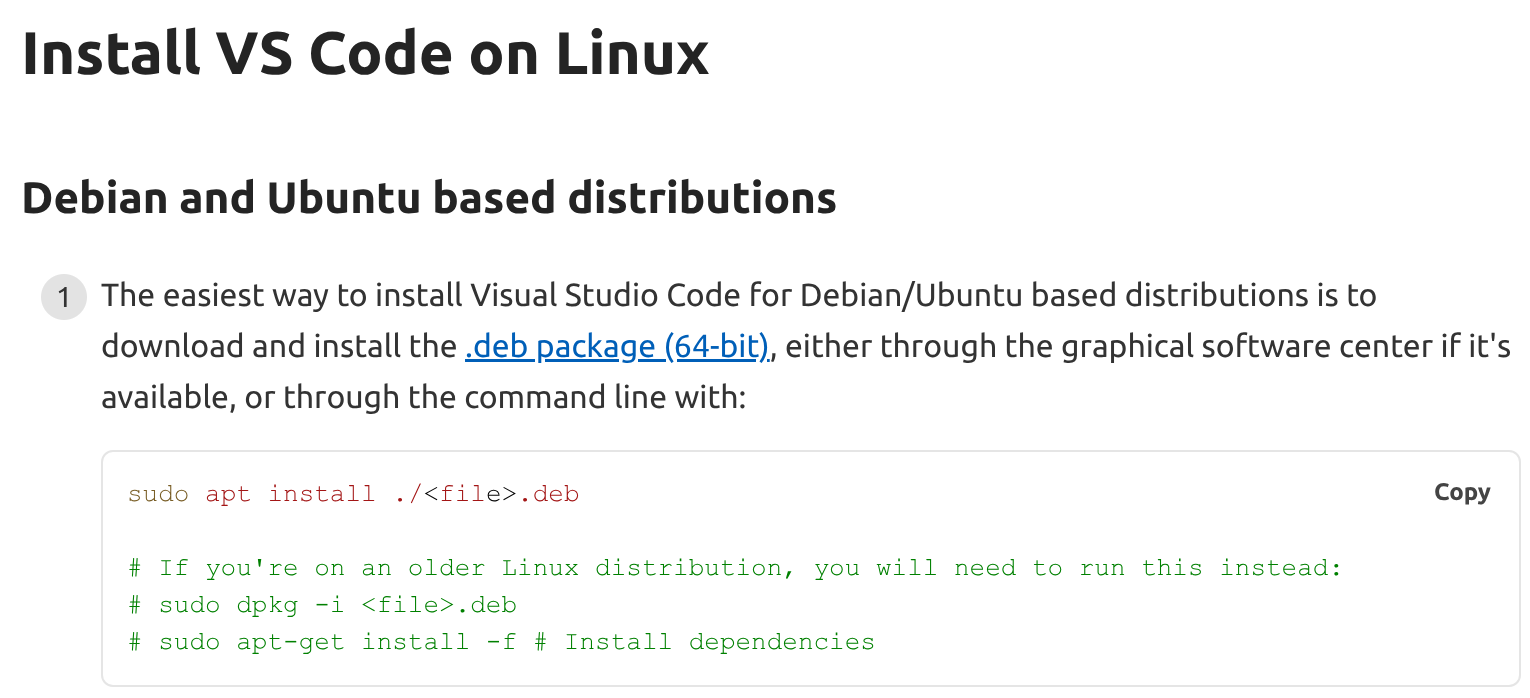
\includegraphics[width=0.9\textwidth]{figs/implementation/install_vscode.png}
            \caption{Installing Visual Studio Code}
            \label{fig:install_vscode}
        \end{figure}
    \item Open Visual Studio Code, follow the example in the tutorial \href{https://code.visualstudio.com/docs/getstarted/getting-started}{Tutorial: Get started with Visual Studio Code}, complete the basic configuration, and open the workspace in the directory \texttt{~/ros2\_ws}. You should see content similar to Figure~\ref{fig:open_ros2_ws}.
        \begin{figure}[!h]
            \centering
            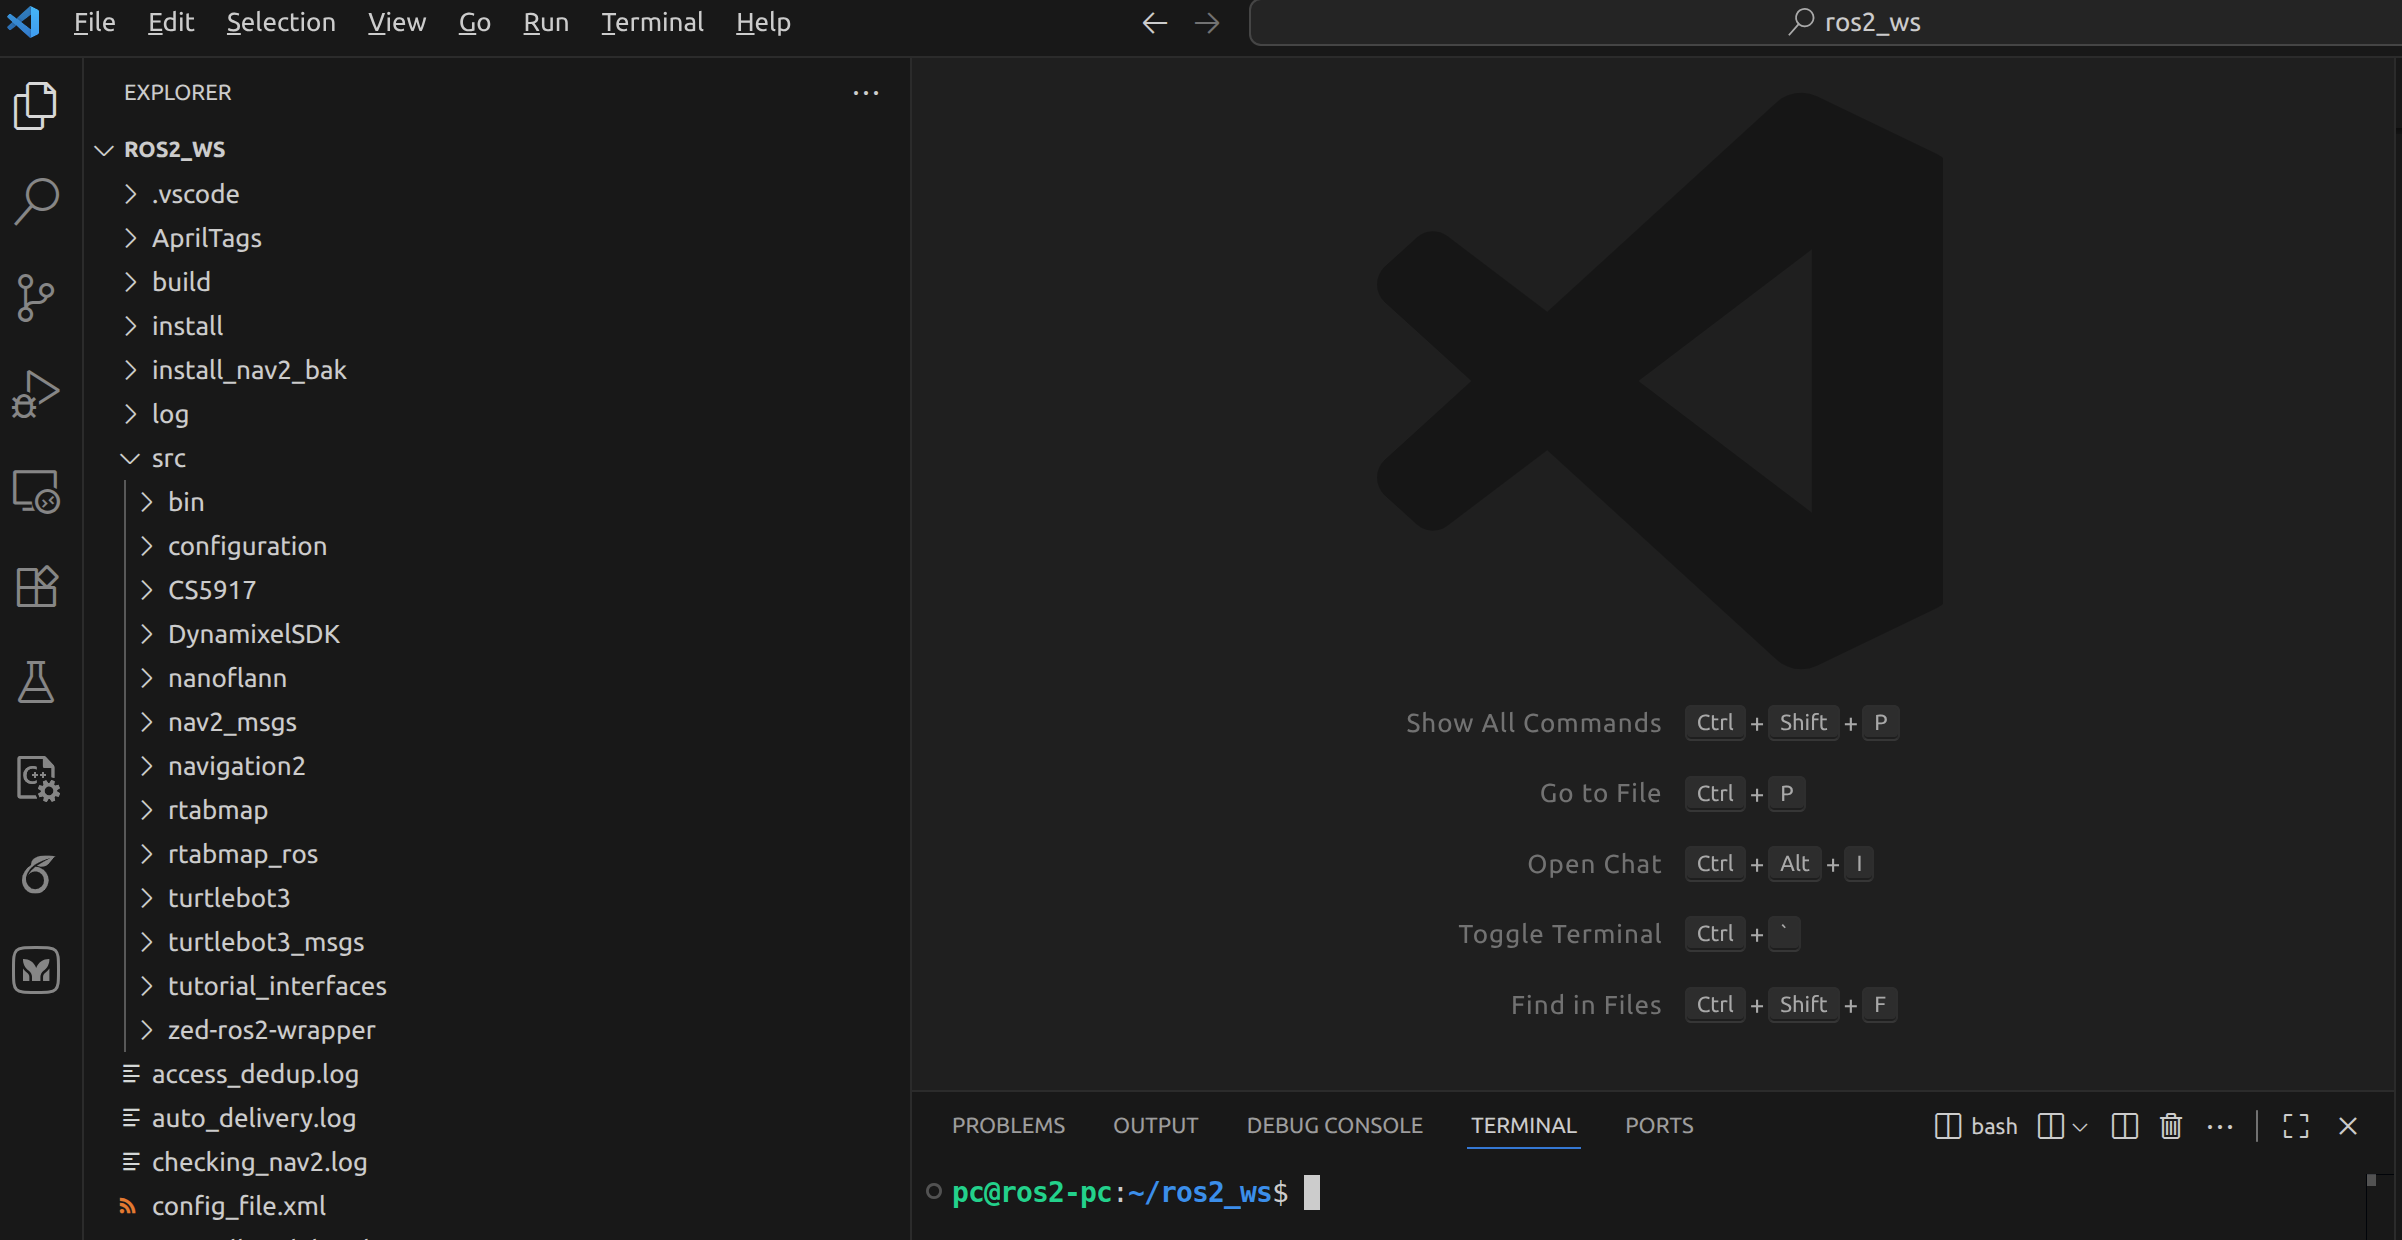
\includegraphics[width=0.9\textwidth]{figs/implementation/open_ros2_ws.png}
            \caption{Opening ROS 2 Workspace}
            \label{fig:open_ros2_ws}
        \end{figure}
\end{enumerate}

\subsubsection{\textbf{Environment Configuration}\label{subsubsec:env_setup}}
[On PC] The relevant configuration commands are as follows:
\begin{lstlisting}[language=bash]
$ echo 'source ~/ros2_ws/install/setup.bash' >> ~/.bashrc
$ echo 'source /opt/ros/humble/setup.bash' >> ~/.bashrc
$ echo "export TURTLEBOT3_MODEL=waffle_pi" >> ~/.bashrc
$ echo 'export ROS_DOMAIN_ID=30 #TURTLEBOT3' >> ~/.bashrc
$ echo 'export RMW_IMPLEMENTATION=rmw_fastrtps_cpp' >> ~/.bashrc
$ source ~/.bashrc
\end{lstlisting}

\subsection{Turtlebot3 Setup\label{subsec:turtlebot3_setup}}
This engineering project uses the Turtlebot3 Waffle Pi version. The specific hardware configuration is shown in Table~\ref{tab:turtlebot3_specs}. For the setup of the Single Board Computer (SBC) and OpenCR on Turtlebot3, please refer to the tutorials \href{https://emanual.robotis.com/docs/en/platform/turtlebot3/sbc_setup/#sbc-setup}{SBC Setup} and \href{https://emanual.robotis.com/docs/en/platform/turtlebot3/opencr_setup/#opencr-setup}{OpenCR Setup}.

\subsection{Jetson Orin Nano Setup\label{subsec:jetson_orin_nano_setup}}
This engineering project uses the Jetson Orin Nano Developer Kit version. The specific hardware configuration is shown in Table~\ref{tab:jetson_orin_nano_specs}. On the Jetson Orin Nano, we mainly install the operating system, ROS 2, ZED SDK, ZED package, rtabmap package, and the engineering package \texttt{uoa\_robot\_drone}, and perform the corresponding environment configuration. Below, we will detail these steps.

\subsubsection{\textbf{Installing the Operating System}\label{subsubsec:jetson_os_setup}}
\begin{enumerate}
    \item After registering a free account according to the tutorial \href{https://docs.nvidia.com/sdk-manager/download-run-sdkm/index.html}{Download and Run SDK Manager}, use the SDK Manager to install Jet Pack version 6.2.1.
    \item Access the graphical interface of the Jetson Orin Nano's Ubuntu system and connect to a wireless network.
    \item To save resources, SSH into the Jetson Orin Nano and enter the command:
    \begin{lstlisting}[language=bash]
        ssh username@ip_address
    \end{lstlisting}
    where \texttt{username} is the username of the Jetson Orin Nano, and \texttt{ip\_address} is the IP address of the Jetson Orin Nano.
    \item After entering the Ubuntu system of the Jetson Orin Nano, enter the command:
    \begin{lstlisting}[language=bash]
        sudo systemctl set-default multi-user.target
        sudo systemctl reboot
    \end{lstlisting}
    \item After rebooting, the Jetson Orin Nano will enter command line mode.
\end{enumerate}

\subsubsection{\textbf{Installing ROS 2}\label{subsubsec:jetson_ros_setup}}
This engineering project uses ROS 2 Humble Hawksbill as the version. Follow the tutorial \href{https://docs.ros.org/en/humble/Installation/Ubuntu-Install-Debs.html}{Ubuntu (deb packages)} to install step by step, and execute the steps shown in Figure~\ref{fig:try_some_examples}.

\subsubsection{\textbf{Installing ZED SDK}\label{subsubsec:zed_sdk_setup}}
This engineering project uses the CUDA 12 ZED SDK for Ubuntu 22 version 5.0. Follow the tutorial \href{https://www.stereolabs.com/docs/development/zed-sdk/linux}{Download and Install the ZED SDK} to install step by step. It is not recommended to install in \texttt{silent mode}.

\subsubsection{\textbf{Installing Packages}\label{subsubsec:jetson_packages_setup}}
On the Jetson Orin Nano, the main packages used in this engineering project are the ZED 2 stereo camera, rtabmap, and the engineering package \texttt{uoa\_robot\_drone}.
[On Jetson Orin Nano] The relevant installation commands are as follows:
\begin{lstlisting}[language=bash]
$ source ~/.bashrc
$ mkdir -p ~/colcon_ws/src
$ cd ~/colcon_ws
$ git clone https://github.com/stereolabs/zed-ros2-wrapper.git src/zed-ros2-wrapper 
$ git clone https://github.com/introlab/rtabmap.git src/rtabmap 
$ git clone -b ros2 https://github.com/introlab/rtabmap_ros.git src/rtabmap_ros
$ git clone -b humble https://github.com/Jian-UOA/CS5917.git src/CS5917
$ sudo apt install python3-colcon-common-extensions
$ colcon build --symlink-install
\end{lstlisting}

\subsubsection{\textbf{Environment Configuration}\label{subsubsec:jetson_env_setup}}
[On Jetson Orin Nano] The relevant configuration commands are as follows:
\begin{lstlisting}[language=bash]
$ echo 'source ~/colcon_ws/install/setup.bash' >> ~/.bashrc
$ echo 'source /opt/ros/humble/setup.bash' >> ~/.bashrc
$ echo 'export ROS_DOMAIN_ID=30' >> ~/.bashrc
$ echo 'export RMW_IMPLEMENTATION=rmw_fastrtps_cpp' >> ~/.bashrc
$ source ~/.bashrc
\end{lstlisting}

\subsubsection{\textbf{Verifying Installation}\label{subsubsec:jetson_verify_setup}}
To verify whether the installation on the Jetson Orin Nano was successful, follow these steps:
\begin{enumerate}
    \item Verify that the ZED 2 camera is successfully installed
        \begin{enumerate}
            \item Open a terminal on the PC, SSH into the Jetson Orin Nano, and enter the command:
                \begin{lstlisting}[language=bash]
                    $ clear && cd ~/colcon_ws && ros2 launch zed_wrapper zed_camera.launch.py | tee zed.log
                \end{lstlisting}
            \item If the ZED-related installation is successful, you should see output similar to Figure~\ref{fig:zed_camera_launch}.
                \begin{figure}[!h]
                    \centering
                    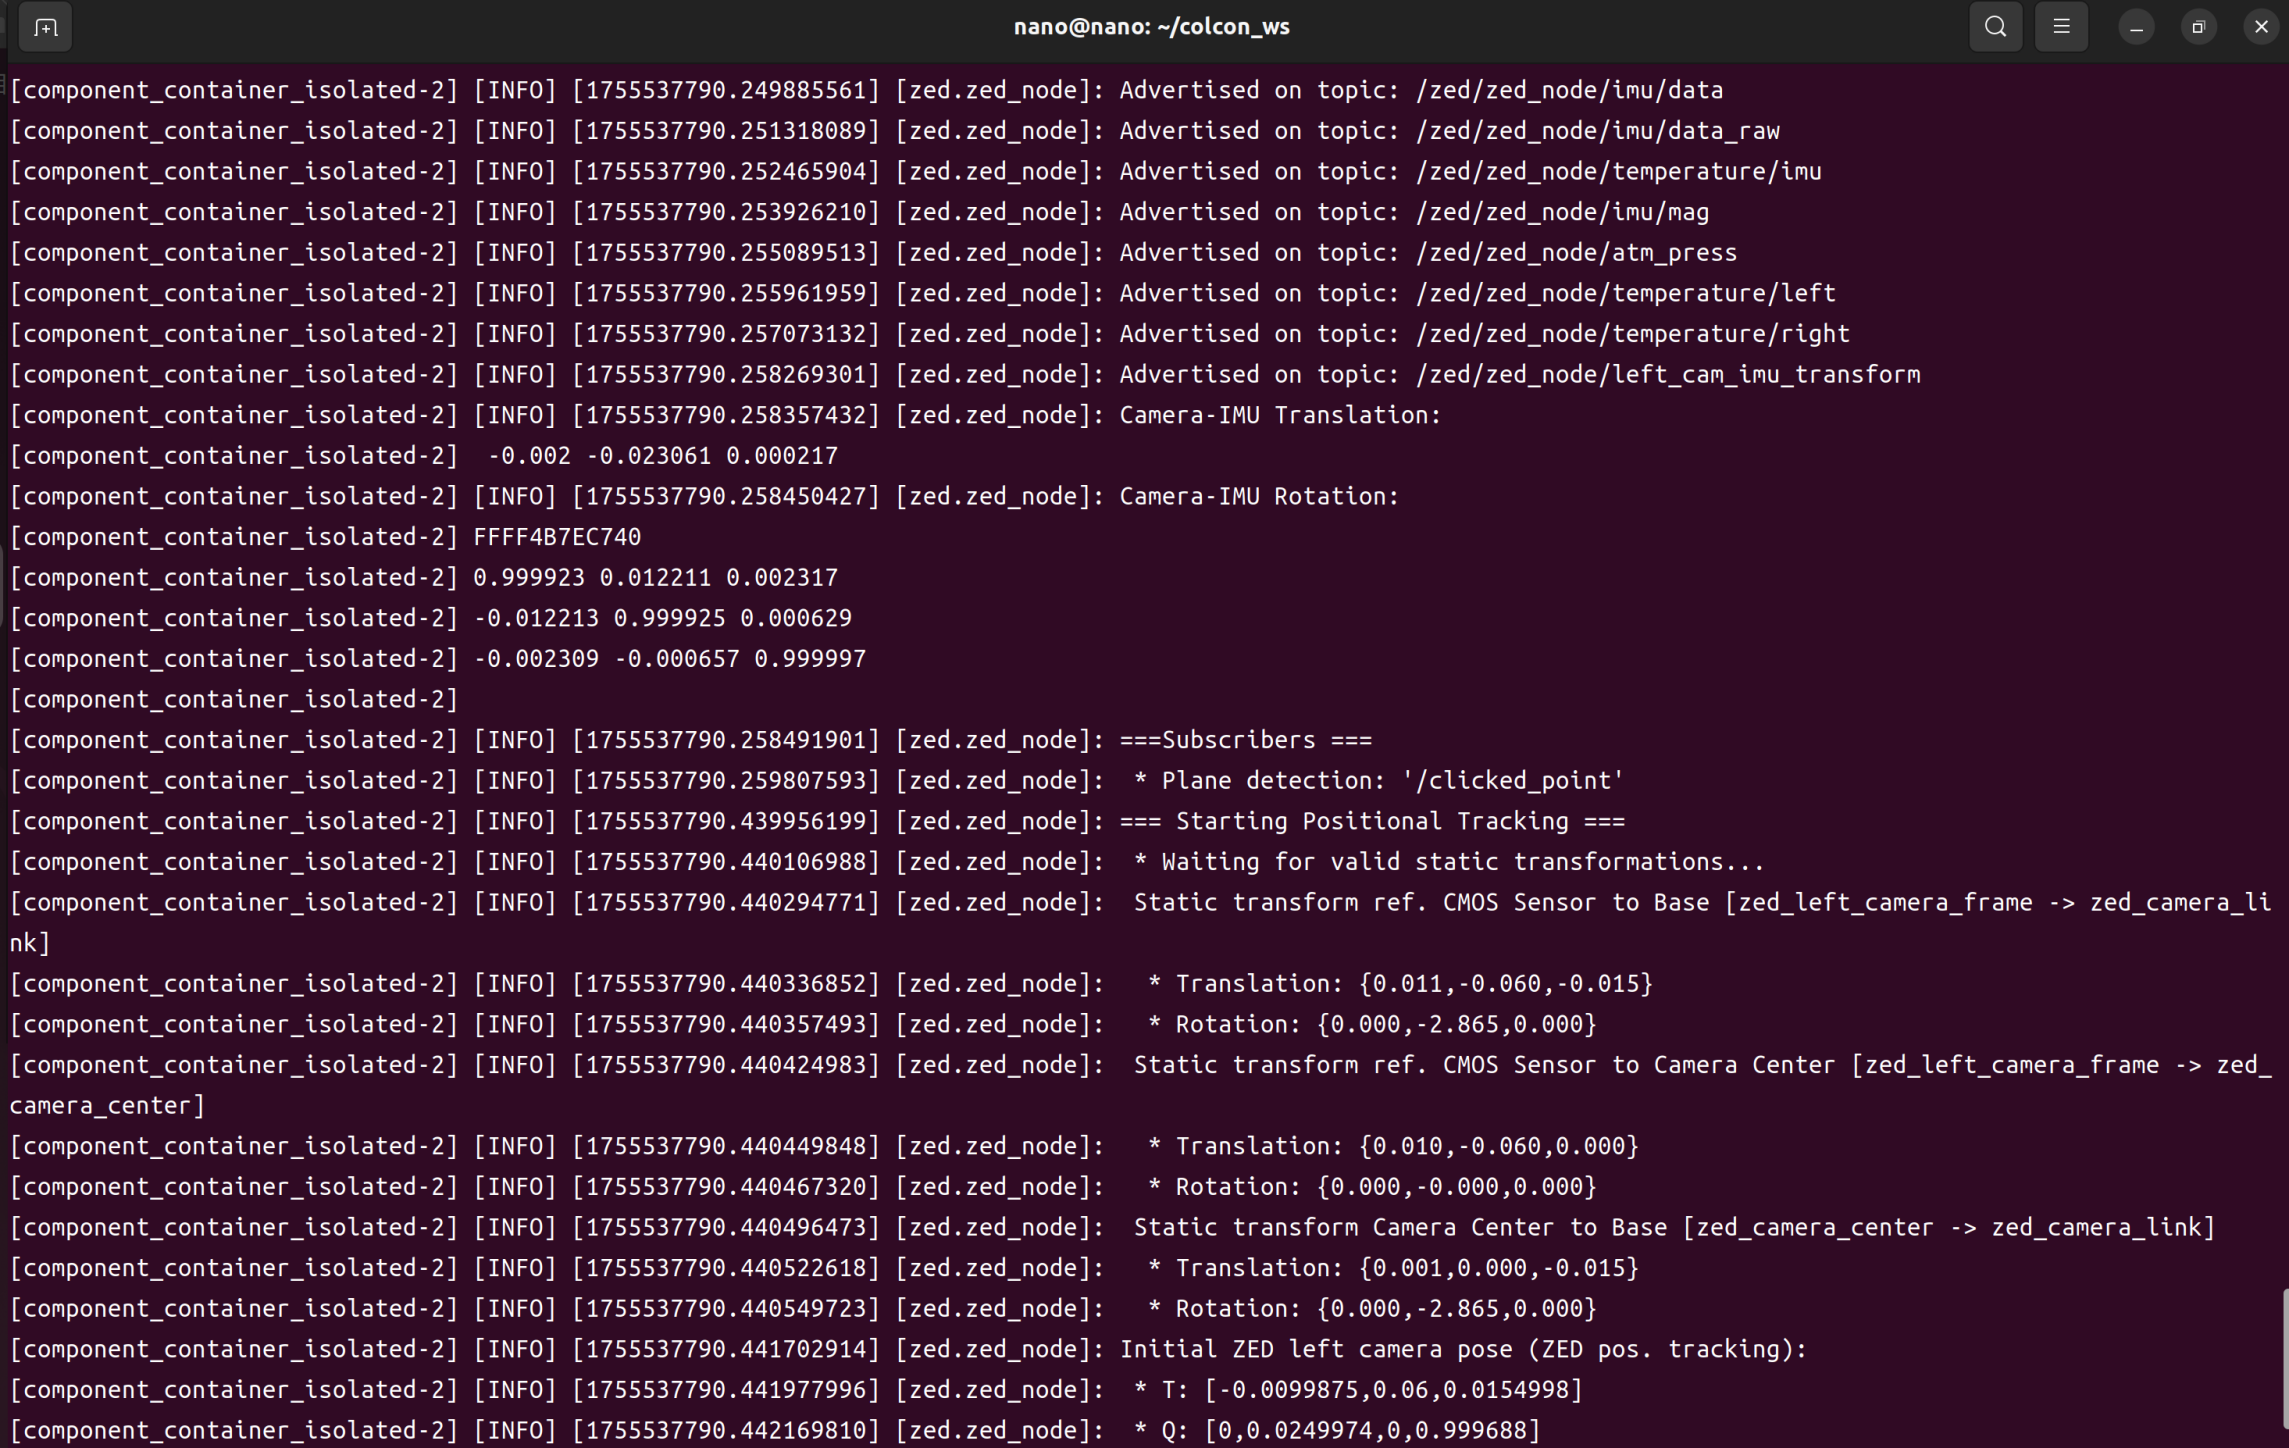
\includegraphics[width=0.9\textwidth]{figs/zed2/zed_camera_launch.png}
                    \caption{ZED Camera Launch Output}
                    \label{fig:zed_camera_launch}
                \end{figure} 
        \end{enumerate}
    \item Verify that the rtabmap package is successfully installed
        \begin{enumerate}
            \item On PC, press \texttt{Ctrl + Alt + T} to open a terminal, SSH into the Jetson Orin Nano, and enter the command:
                \begin{lstlisting}[language=bash]
                    $ clear && cd ~/colcon_ws && ros2 launch uoa_robot_drone orin_stereo_vslam.launch.py localization:=false | tee orin_vslam.log
                \end{lstlisting}
            \item If the rtabmap\-related installation is successful, you should see output similar to Figure~\ref{fig:orin_stereo_vslam_launch}.
                \begin{figure}[!h]
                    \centering
                    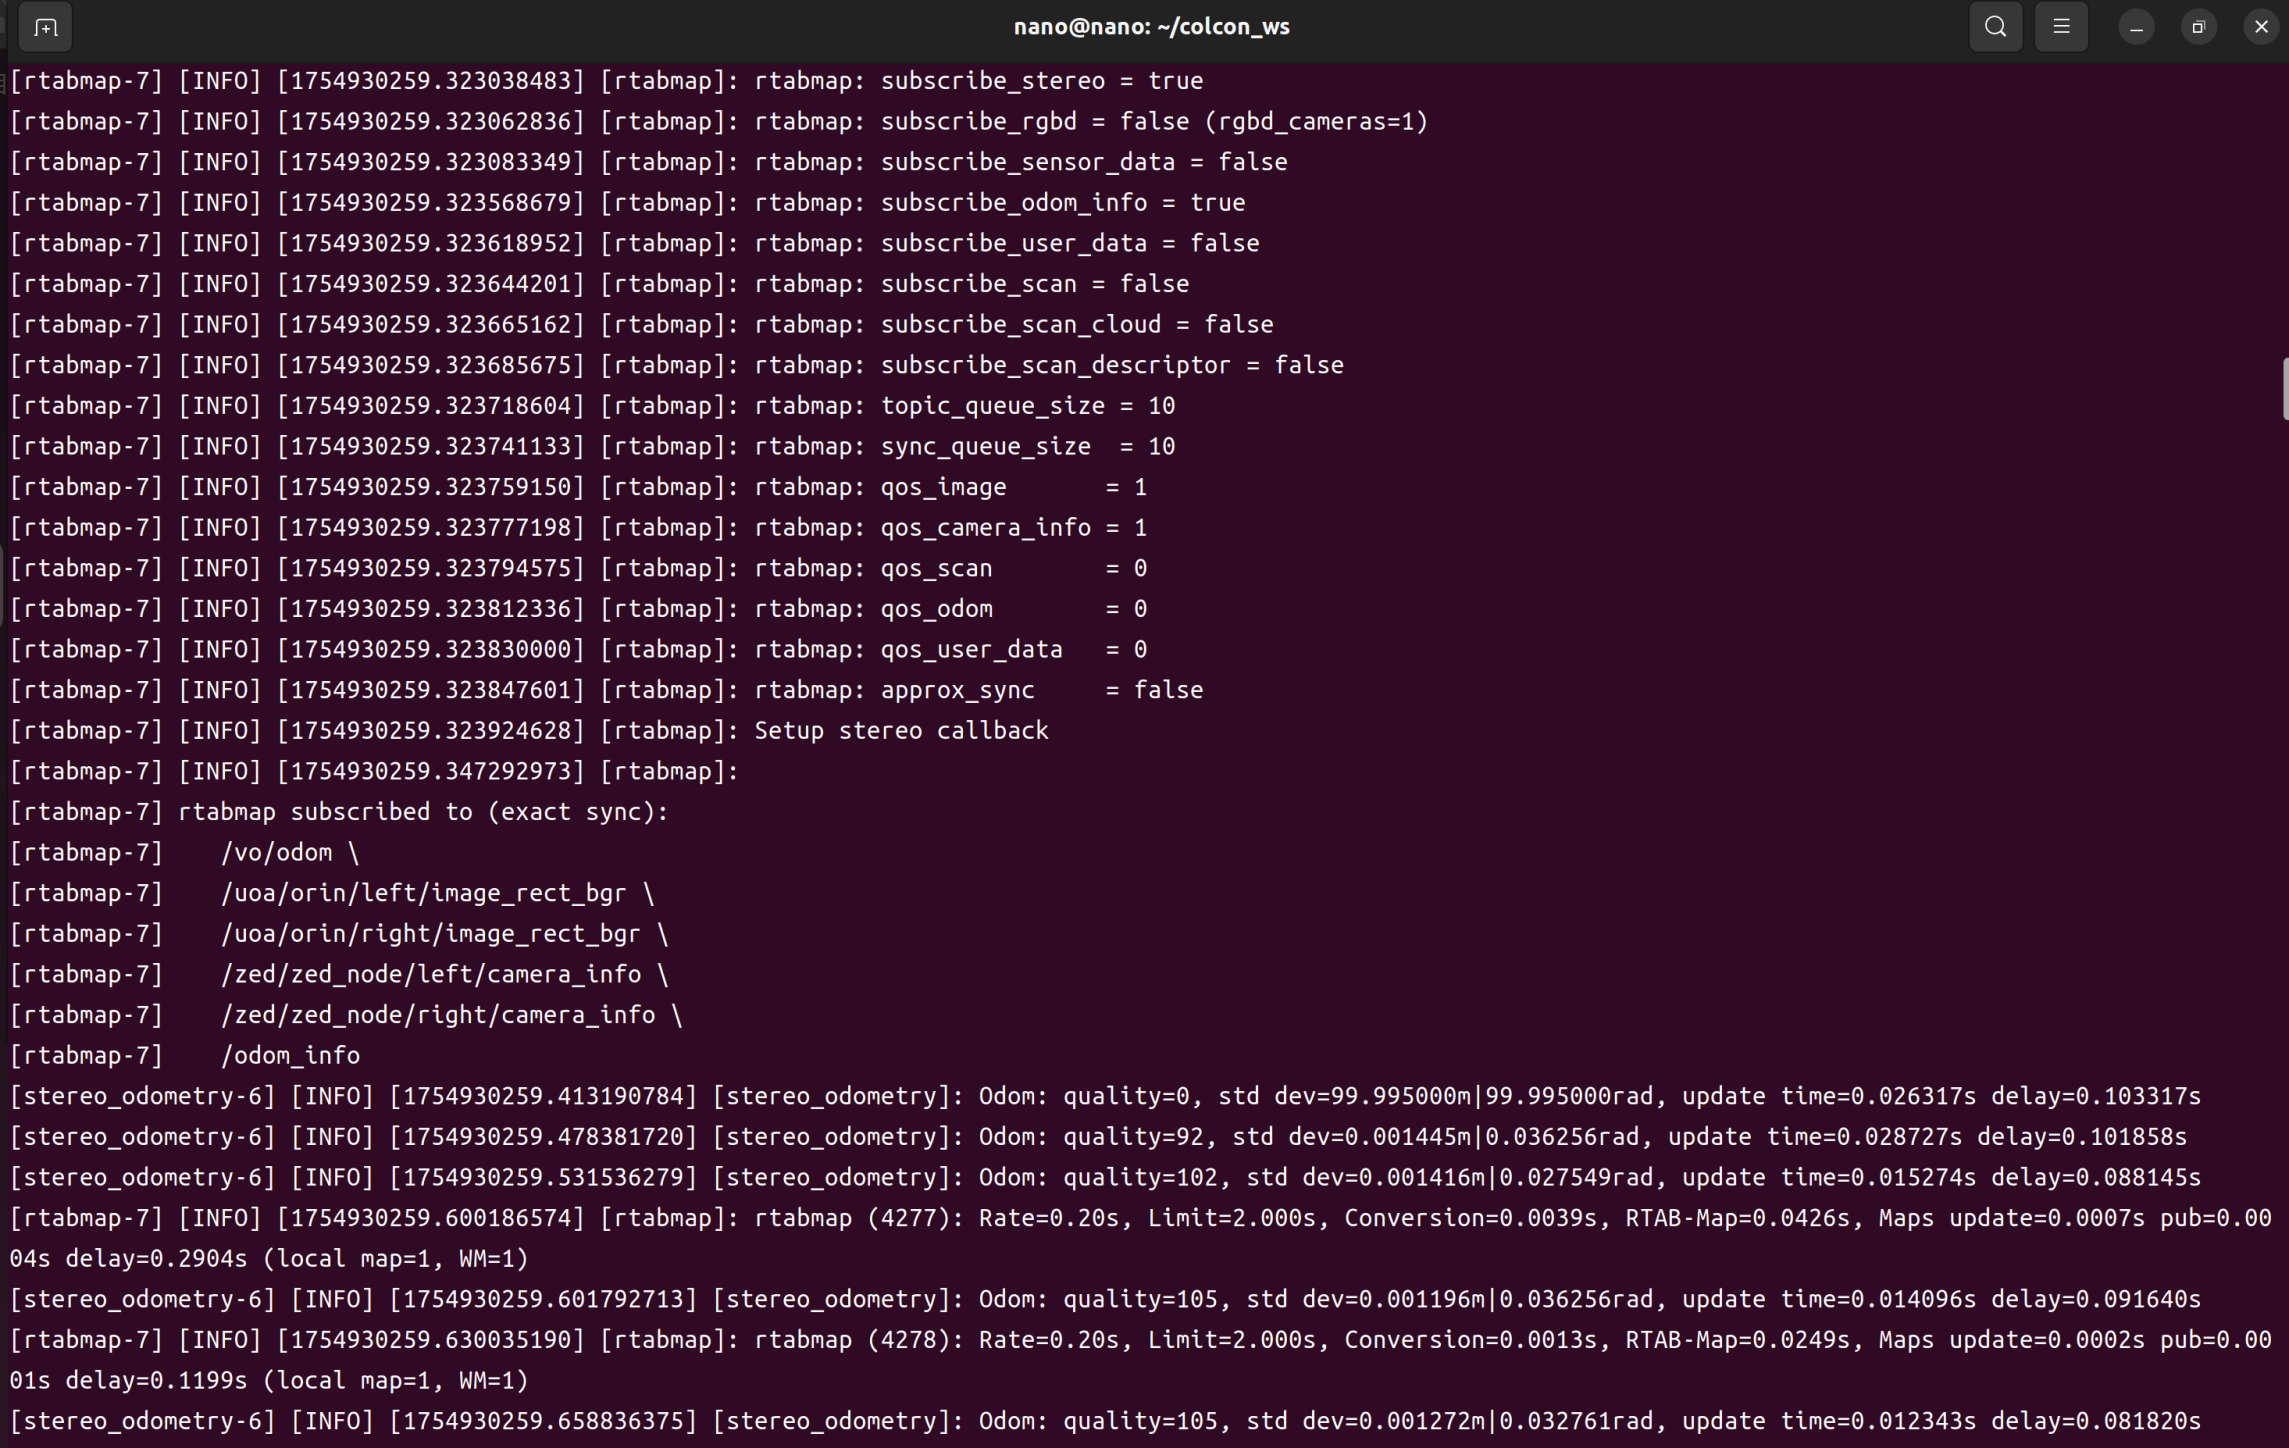
\includegraphics[width=0.9\textwidth]{figs/orin/orin_stereo_vslam_launch.png}
                    \caption{Orin Stereo Visual SLAM Launch Output}
                    \label{fig:orin_stereo_vslam_launch}
                \end{figure}
        \end{enumerate}
\end{enumerate}
\include{evaluation}
\include{conclusion}


\bibliography{references}

\appendix
% \include{proof}


\chapter{ROS Graphs}
\label{app:ros2graphs}
In ROS, the communication between nodes is facilitated through a system of topics, services, and actions. The ROS 2 graph is a representation of this communication network, showing how nodes are connected and how they exchange messages.
Here are some ROS graphs from different stages of the engineering.

\section{ROS Graph of the Mapping Stage}
\label{subsec:rosgraph_mapping}
\newgeometry{left=2cm,right=1cm,top=1cm,bottom=0.05cm}
\begin{landscape}
    \thispagestyle{empty}
    \begin{figure}[p]
        \centering
        
\includegraphics[height=0.69\textwidth]{figs/ros_graphs/mapping_stage_rosgraph.png}
        \caption{ROS Graph of the Mapping Stage}
        \label{fig:rosgraph_mapping}
    \end{figure}
\end{landscape}
\restoregeometry

\section{ROS Graph of the Localization Stage}
\label{subsec:rosgraph_localization}
\newgeometry{left=1cm,right=2.9cm,top=1cm,bottom=1cm}
\begin{landscape}
    \thispagestyle{empty}
    \begin{figure}[p]
        \centering
        
\includegraphics[height=0.75\textwidth]{figs/ros_graphs/localization_stage_rosgraph.png}
        \caption{ROS Graph of the Localization Stage}
        \label{fig:rosgraph_localization}
    \end{figure}
\end{landscape}
\restoregeometry

\section{ROS Graph of the Navigation Stage}
\label{subsec:rosgraph_navigation}
\newgeometry{left=0.5cm,right=3.6cm,top=1cm,bottom=0.05cm}
\begin{landscape}
    \thispagestyle{empty}
    \begin{figure}[p]
        \centering
        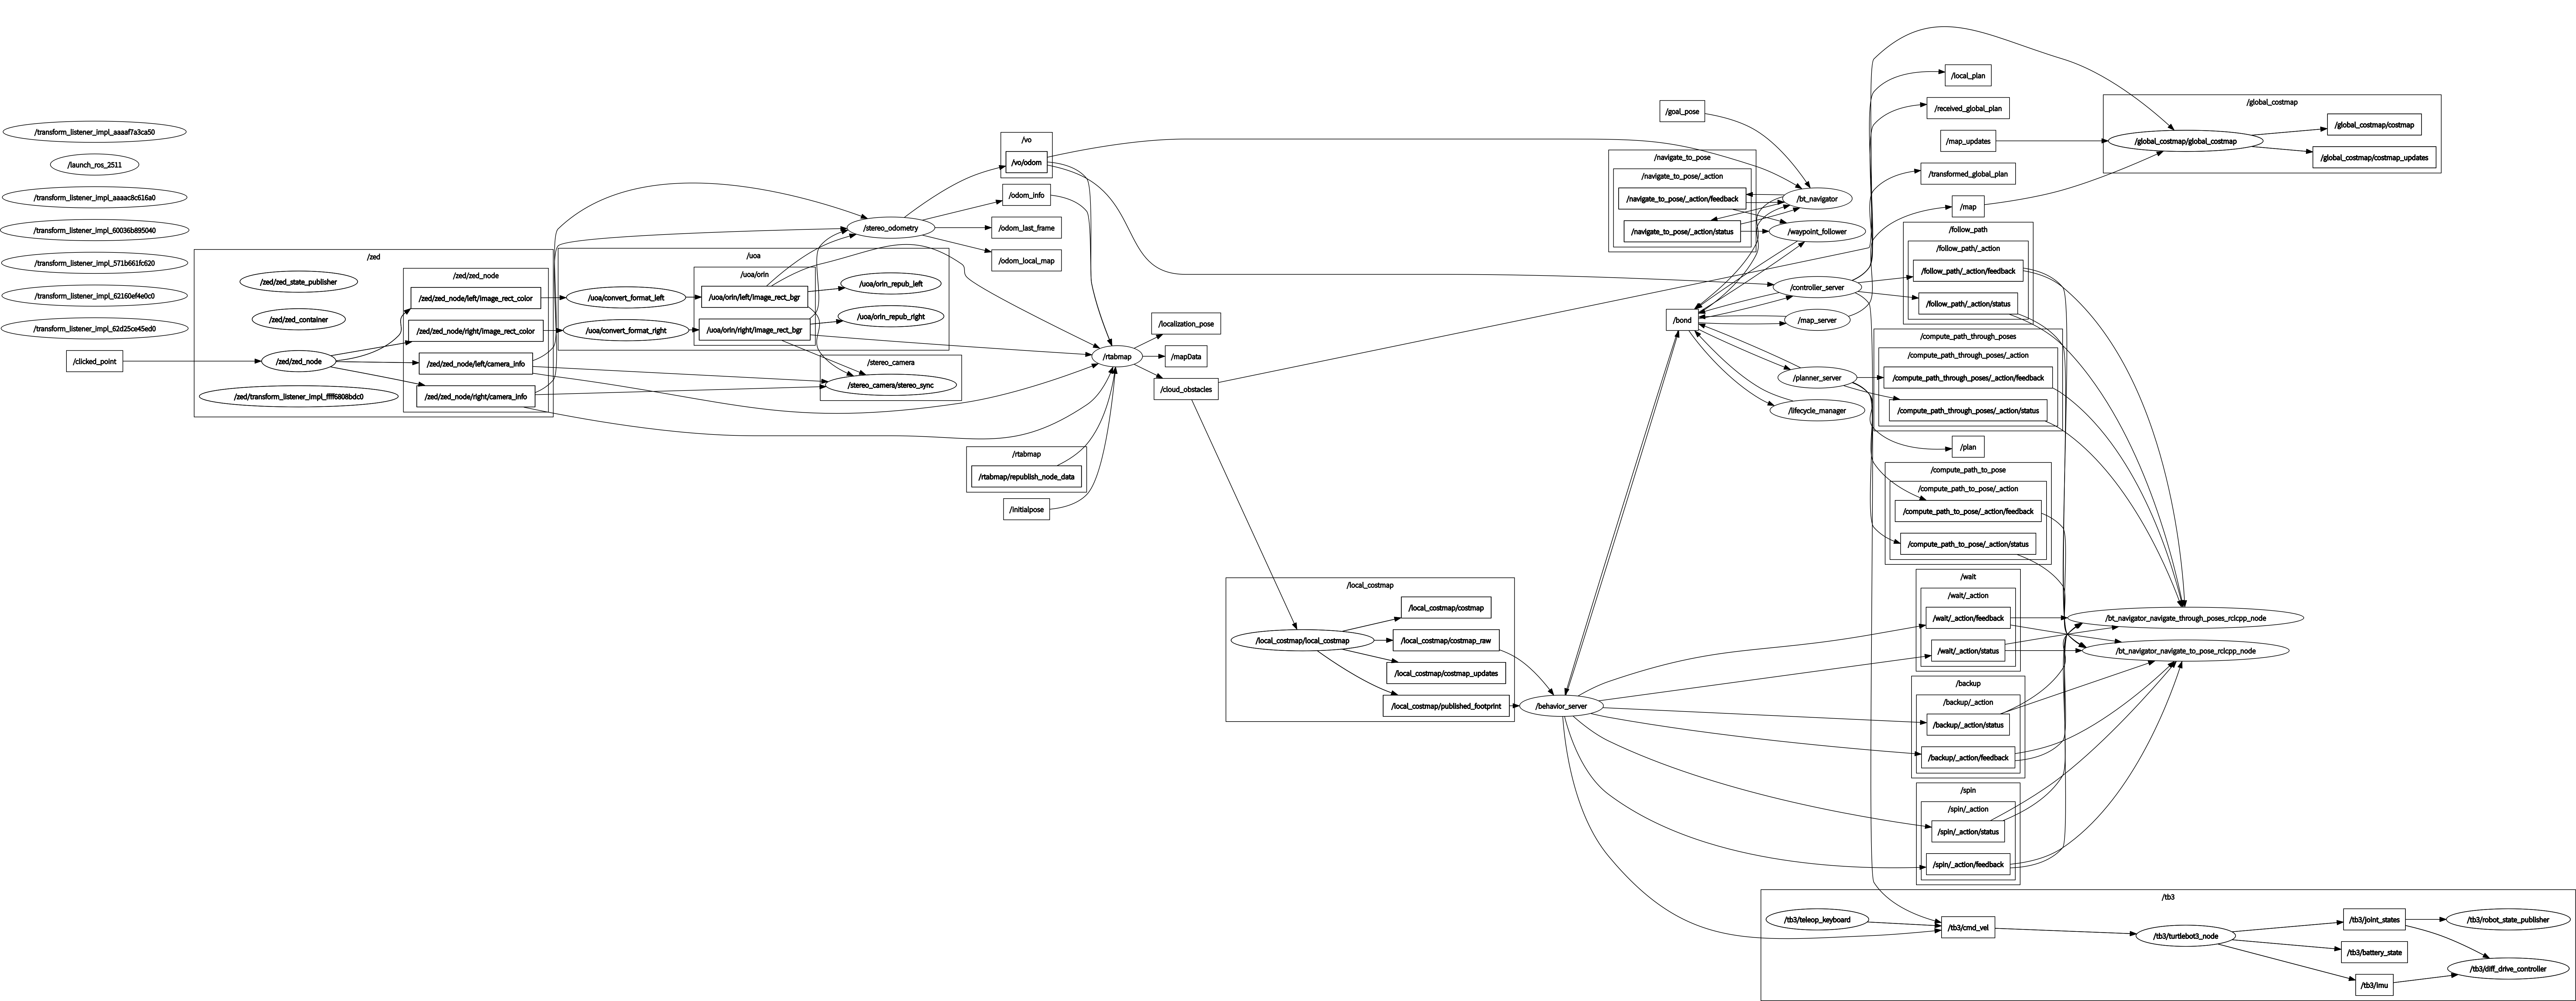
\includegraphics[height=0.68\textwidth]{figs/ros_graphs/navigation_stage_rosgraph.png}
        \caption{ROS Graph of the Navigation Stage}
        \label{fig:rosgraph_navigation}
    \end{figure}
\end{landscape}
\restoregeometry

\chapter{Hardware Specifics\label{chap:hardware_specifics}}
\section{Turtlebot3 Waffle Pi Details}\label{sec:turtlebot3_details}
This section provides detailed specifications and component lists for Turtlebot3 Waffle Pi used in this project.
\begin{table}[htbp]
	\centering
	\caption{Turtlebot3 Waffle Pi Technical Specifications}
	\label{tab:turtlebot3_specs}
	\begin{tabular}{|l|p{8cm}|}
		\hline
			extbf{Specification} & \textbf{Waffle Pi} \\
		\hline
		Maximum translational velocity & 0.26 m/s \\
		\hline
		Maximum rotational velocity & 1.82 rad/s (104.27 deg/s) \\
		\hline
		Maximum payload & 30kg \\
		\hline
		Size (L $\times$ W $\times$ H) & 281mm $\times$ 306mm $\times$ 141mm \\
		\hline
		Weight (+ SBC + Battery + Sensors) & 1.8kg \\
		\hline
		Climbing Threshold & 10 mm or lower \\
		\hline
		Expected operating time & 2h \\
		\hline
		Expected charging time & 2h 30m \\
		\hline
		SBC (Single Board Computer) & Raspberry Pi 4 \\
		\hline
		MCU & 32-bit ARM Cortex\textregistered-M7 with FPU (216 MHz, 462 DMIPS) \\
		\hline
		Remote Controller & RC-100B + BT-410 Set (Bluetooth 4, BLE) \\
		\hline
		Actuator & XM430-W210 \\
		\hline
		LDS (Laser Distance Sensor) & 360 Laser Distance Sensor LDS-02 \\
		\hline
		Camera & Raspberry Pi Camera Module v2.1 \\
		\hline
		IMU & Gyroscope 3 Axis, Accelerometer 3 Axis \\
		\hline
		Power connectors & 3.3V / 800mA, 5V / 4A, 12V / 1A \\
		\hline
		Expansion pins & GPIO 18 pins, Arduino 32 pin \\
		\hline
		Peripheral Connections & UART $\times$3, CAN $\times$1, SPI $\times$1, I2C $\times$1, ADC $\times$5, 5pin OLLO $\times$4 \\
		\hline
		DYNAMIXEL ports & RS485 $\times$ 3, TTL $\times$ 3 \\
		\hline
		Audio & Several programmable beep sequences \\
		\hline
		Programmable LEDs & User LED $\times$ 4 \\
		\hline
		Status LEDs & Board status LED $\times$ 1, Arduino LED $\times$ 1, Power LED $\times$ 1 \\
		\hline
		Buttons and Switches & Push buttons $\times$ 2, Reset button $\times$ 1, Dip switch $\times$ 2 \\
		\hline
		Battery & Lithium polymer 11.1V 1800mAh / 19.98Wh 5C \\
		\hline
		PC Connection & USB \\
		\hline
		Firmware Upgrade & via USB / via JTAG \\
		\hline
		Power Adapter (SMPS) & Input: 100-240V, AC 50/60Hz, 1.5A @max; Output: 12V DC, 5A \\
		\hline
	\end{tabular}
\end{table}
\begin{table}[htbp]
	\centering
	\caption{Turtlebot3 Waffle Pi Components List}
	\label{tab:turtlebot3_components_list}
	\begin{tabular}{|m{3.5cm}|l|c|}
	\hline
		extbf{Category} & \textbf{Part Name} & \textbf{Quantity} \\
	\hline
	Chassis Parts & Waffle Plate & 24 \\
	\cline{2-3} & Plate Support M3$\times$35mm & 12 \\
	\cline{2-3} & Plate Support M3$\times$45mm & 10 \\
	\cline{2-3} & PCB Support & 12 \\
	\cline{2-3} & Wheel & 2 \\
	\cline{2-3} & Tire & 2 \\
	\cline{2-3} & Ball Caster & 2 \\
	\cline{2-3} & Camera Bracket & 1 \\
	\hline
	Motors & DYNAMIXEL (XM430-W210-T) & 2 \\
	\hline
	Boards & OpenCR1.0 & 1 \\
	\cline{2-3} & Raspberry Pi & 1 \\
	\cline{2-3} & USB2LDS & 1 \\
	\hline
	Remote Controllers & BT-410 Set (Bluetooth 4, BLE) & 1 \\
	\cline{2-3} & RC-100B (Remote Controller) & 1 \\
	\hline
	Sensors & LDS-01 or LDS-02 & 1 \\
	\cline{2-3} & Raspberry Pi Camera v2.1 & 1 \\
	\hline
	Memory & MicroSD Card & 1 \\
	\hline
	Cables & Raspberry Pi Power Cable & 1 \\
	\cline{2-3} & Li-Po Battery Extension Cable & 1 \\
	\cline{2-3} & DYNAMIXEL to OpenCR Cable & 2 \\
	\cline{2-3} & USB Cable & 2 \\
	\cline{2-3} & Camera Cable & 1 \\
	\hline
	Powers & SMPS 12V5A & 1 \\
	\cline{2-3} & A/C Cord & 1 \\
	\cline{2-3} & LIPO Battery 11.1V 1,800mAh & 1 \\
	\cline{2-3} & LIPO Battery Charger & 1 \\
	\hline
	Tools & Screw driver & 1 \\
	\cline{2-3} & Rivet tool & 1 \\
	\hline
	Miscellaneous & PH\_M2$\times$4mm\_K & 8 \\
	\cline{2-3} & PH\_T2$\times$6mm\_K & 8 \\
	\cline{2-3} & PH\_M2$\times$12mm\_K & 4 \\
	\cline{2-3} & PH\_M2.5$\times$8mm\_K & 16 \\
	\cline{2-3} & PH\_M2.5$\times$12mm\_K & 20 \\
	\cline{2-3} & PH\_M2.5$\times$16mm\_K & 4 \\
	\cline{2-3} & PH\_M3$\times$8mm\_K & 140 \\
	\cline{2-3} & NUT\_M2 & 4 \\
	\cline{2-3} & NUT\_M2.5 & 24 \\
	\cline{2-3} & NUT\_M3 & 96 \\
	\cline{2-3} & Rivet\_1 & 22 \\
	\cline{2-3} & Rivet\_2 & 2 \\
	\cline{2-3} & Spacer & 4 \\
	\cline{2-3} & Silicone Spacer & 4 \\
	\cline{2-3} & Bracket & 6 \\
	\cline{2-3} & Adapter Plate & 1 \\
	\hline
	\end{tabular}
\end{table}

\section{ZED 2 Stereo Vision Camera Details}\label{sec:zed2_details}
This section provides detailed specifications for the ZED 2 stereo vision camera used in this project.
\begin{table}[htbp]
	\centering
	\caption{ZED 2 Technical Specifications}
	\label{tab:zed2_specs}
	\begin{tabular}{|l|p{8cm}|}
		\hline
			extbf{Specification} & \textbf{Value} \\
		\hline
		Resolution & 2.2K at 15 FPS, 1080p at 30 or 15 FPS, 720p at 60, 30 or 15 FPS, 376p at 100, 60, 30 or 15 FPS \\
		\hline
		Field of View & Horizontal: 110°, Vertical: 70°, Diagonal: 120° max. \\
		\hline
		Baseline & 120 mm (4.72'') \\
		\hline
		Dimensions & 175 x 30 x 33 mm (6.89 x 1.18 x 1.3'') \\
		\hline
		Weight & 124 g (0.27 lb) \\
		\hline
	\end{tabular}
\end{table}
\begin{table}[htbp]
	\centering
	\caption{ZED 2 Mechanical Parameters}
	\label{tab:zed2_mechanical}
	\begin{tabular}{|l|l|}
		\hline
			extbf{Parameter} & \textbf{Value} \\
		\hline
		Baseline & 120 mm (4.72'') \\
		\hline
		Dimensions & 175 x 30 x 33 mm (6.89 x 1.18 x 1.3'') \\
		\hline
		Weight & 124 g (0.27 lb) \\
		\hline
	\end{tabular}
\end{table}
\begin{table}[htbp]
	\centering
	\caption{ZED 2 Video Output Parameters}
	\label{tab:zed2_video_output}
	\begin{tabular}{|l|p{8cm}|}
		\hline
			extbf{Parameter} & \textbf{Value} \\
		\hline
		Video Output & Stereo-rectified, side-by-side, or anaglyphic video stream \\
		\hline
		Video Output Resolutions & 2.2K at 15 FPS, 1080p at 30 or 15 FPS, 720p at 60, 30 or 15 FPS, 376p at 100, 60, 30 or 15 FPS \\
		\hline
		Video Recording Formats & H.264, H.265, or lossless format (on host) \\
		\hline
		Video Streaming & Stream anywhere over IP using ZED SDK \\
		\hline
	\end{tabular}
\end{table}
\begin{table}[htbp]
	\centering
	\caption{ZED 2 Lens Parameters}
	\label{tab:zed2_lens}
	\begin{tabular}{|l|p{8cm}|}
		\hline
			extbf{Parameter} & \textbf{Value} \\
		\hline
		Lens Type & Wide-angle 8-element all-glass dual lens with optically corrected distortion \\
		\hline
		Aperture & ƒ/2.0 \\
		\hline
		Focal Length & 2.12 mm (0.08'') \\
		\hline
		Field of View & 110° (H) x 70° (V) x 120° (D) max. \\
		\hline
		Polarizing Filter & None \\
		\hline
	\end{tabular}
\end{table}
\begin{table}[htbp]
	\centering
	\caption{ZED 2 Image Sensors Parameters}
	\label{tab:zed2_image_sensors}
	\begin{tabular}{|l|p{8cm}|}
		\hline
			extbf{Parameter} & \textbf{Value} \\
		\hline
		Sensor Resolution & Dual 4M pixels sensors with 2-micron pixels \\
		\hline
		Sensor Format & Native 16:9 format for a greater horizontal field of view \\
		\hline
		Sensor Size & 1/3" backside illumination sensors with high low-light sensitivity \\
		\hline
		Shutter Sync & Electronic Synchronized Rolling Shutter \\
		\hline
	\end{tabular}
\end{table}
\begin{table}[htbp]
	\centering
	\caption{ZED 2 Connectivity Parameters}
	\label{tab:zed2_connectivity}
	\begin{tabular}{|l|p{8cm}|}
		\hline
			extbf{Parameter} & \textbf{Value} \\
		\hline
		Connector & USB 3.0 port with 1.2m integrated cable \\
		\hline
		Mounting Options & 1/4"-20 UNC thread mount, 2x M3 threads \\
		\hline
		Power & Power via USB 5V / 380mA \\
		\hline
		Operating Temperature & -10°C to +50°C (14°F to 122°F) \\
		\hline
	\end{tabular}
\end{table}

\section{INIU Power Bank Details}\label{sec:iniu_details}
This section provides detailed specifications for the INIU 65W 20000mAh Power Bank used in this project.
\begin{table}[htbp]
	\centering
	\caption{INIU Power Bank Technical Specifications}
	\label{tab:iniu_power_bank_specs}
	\begin{tabular}{|l|l|}
		\hline
			extbf{Specification} & \textbf{Value} \\
		\hline
		Brand & INIU \\
		\hline
		Batteries & 1 Lithium Polymer battery \\
		\hline
		Capacity & 20000 milliamp hours \\
		\hline
		Connector Type & USB Type C $\times$ 2, USB Type A $\times$ 1 \\
		\hline
		Number of Ports & 3 \\
		\hline
		Product Dimensions & 15 x 17.4 x 2.8 cm \\
		\hline
		Weight & 480 g \\
		\hline
		Voltage & 20 volts \\
		\hline
		Manufacturer & Shenzhen Topstar Industry Co., Ltd. \\
		\hline
		ASIN & B0CB1DF4JQ \\
		\hline
		Item Model Number & BI-B62 \\
		\hline
		Country of Origin & China \\
		\hline
	\end{tabular}
\end{table}

\section{DJI Tello EDU Drone Details}\label{sec:tello_details}
This section provides detailed specifications for the DJI Tello EDU drone used in this project.
\begin{table}[htbp]
	\centering
	\caption{DJI Tello EDU Technical Specifications}
	\label{tab:tello_edu_specs}
	\begin{tabular}{|l|p{9cm}|}
		\hline
			extbf{Specification} & \textbf{Value} \\
		\hline
		Weight & 87 g (0.19 lb) \\
		\hline
		Dimensions & 98 mm $\times$ 92.5 mm $\times$ 41 mm (3.86'' $\times$ 3.64'' $\times$ 1.61'') \\
		\hline
		Max Flight Time & Approximately 13 minutes (with full battery) \\
		\hline
		Max Flight Distance & Approximately 100 m (328 ft) in open space \\
		\hline
		Camera Resolution & 5 MP, supports HD video recording at 720p @30fps \\
		\hline
		Battery Capacity & 1100 mAh, rechargeable via Micro USB port \\
		\hline
		Control Range & Up to 100 m (328 ft) with Wi-Fi connection \\
		\hline
		Operating Temperature Range & -10°C to +40°C (14°F to 104°F) \\
		\hline
		Built-in Functions & Range Finder, Barometer, LED, Vision System, 2.4 GHz 802.11n Wi-Fi \\
		\hline
	\end{tabular}
\end{table}

\section{Lenovo Laptop Yoga 14s 2021 Details}\label{sec:lenovo_details}
This section provides detailed specifications for the Lenovo Laptop Yoga 14s 2021 used in this project.
\begin{table}[htbp]
	\centering
	\caption{Lenovo Yoga 14s 2021 Technical Specifications}
	\label{tab:lenovo_laptop_specs}
	\begin{tabular}{|l|l|p{6.5cm}|}
		\hline
			extbf{Category} & \textbf{Specification} & \textbf{Value} \\
		\hline
		{CPU} & CPU Model & Intel Core i5-11300H (11th Generation) \\
		\cline{2-3} & Base Frequency & 3.1 GHz \\
		\cline{2-3} & Max Frequency & 4.40 GHz \\
		\cline{2-3} & Cache & 8 MB \\
		\cline{2-3} & Core Count & 4 \\
		\cline{2-3} & Thread Count & 8 \\
		\cline{2-3} & Chipset & Tiger Lake \\
		\hline
		{Storage} & Standard Memory & 16GB, LPDDR4X 4266MHz \\
		\cline{2-3} & Maximum Memory (Factory) & 16GB \\
		\cline{2-3} & Maximum Memory (Supported) & N/A \\
		\cline{2-3} & Hard Drive & M.2 2280 NVME 512GB SSD \\
		\cline{2-3} & Optical Drive & None \\
		\cline{2-3} & Memory Slots & 0 \\
		\hline
		{Graphics} & Integrated Graphics & Intel Iris Xe Graphics \\
		\cline{2-3} & Discrete Graphics & NVIDIA GeForce MX450 \\
		\cline{2-3} & VRAM Type & GDDR6 \\
		\cline{2-3} & VRAM Capacity & 2GB \\
		\hline
		{Display} & Screen Size & 14 inches \\
		\cline{2-3} & Aspect Ratio & 16:10 \\
		\cline{2-3} & Resolution & 2880 x 1800 \\
		\cline{2-3} & Screen Type & LED Backlight \\
		\hline
		{Multimedia} & Camera & Infrared-enabled Camera \\
		\cline{2-3} & Microphone & Array Microphone \\
		\cline{2-3} & Speaker & Built-in Speaker \\
		\hline
		{Power} & External Power & None \\
		\cline{2-3} & Battery & 4-cell Battery (61Wh) \\
		\hline
		{Connectivity} & Ethernet & N/A \\
		\cline{2-3} & Wireless Card & WiFi 6 Protocol Compatible \\
		\cline{2-3} & Bluetooth & Yes (Integrated with Wireless Card) \\
		\hline
	\end{tabular}
\end{table}


\end{document}
